\documentclass[journal,onecolumn]{IEEEtran}
% \documentclass[journal]{IEEEtran}

\usepackage[hidelinks]{hyperref}
\usepackage{graphicx}
\usepackage{xcolor}
\usepackage{tabularx}
\usepackage{amsmath,amssymb,amsbsy,amsfonts}
\usepackage{accents}
\usepackage{nicefrac}
\usepackage{upgreek}
\usepackage[]{footmisc}

% !TEX root=root.tex

% vectors, quaternions, etc.
\newcommand*{\vect}[1]{\boldsymbol{\mathrm{#1}}}
\newcommand*{\quat}[1]{\boldsymbol{\mathrm{#1}}}

\newcommand*{\x}{\vect{x}}
\newcommand*{\xt}{\tilde{\vect{x}}}
\newcommand*{\xhat}{\hat{\vect{x}}}
\newcommand*{\xbar}{\bar{\vect{x}}}

\newcommand*{\z}{\vect{z}}
\newcommand*{\zhat}{\hat{\vect{z}}}
\newcommand*{\zbar}{\bar{\vect{z}}}

\newcommand*{\q}{\quat{q}}
\newcommand*{\e}{\vect{e}}
\newcommand*{\qt}{\tilde{\quat{q}}}
\newcommand*{\drag}{c_d}

% modifiers
% \newcommand*{\desired}[1]{\accentset{\circ}{#1}}
\newcommand*{\des}[1]{\check{#1}}

% norms, transpose, etc.
\newcommand*{\transpose}{\mathsf{T}}
\newcommand*{\skewmat}[1]{\left[ #1 \right]_{\times}}
\newcommand*{\norm}[1]{\left\Vert #1\right\Vert }
\newcommand*{\abs}[1]{\left\vert #1\right\vert }

% group/algebra names
\newcommand*{\SO}{\ensuremath{\mathit{SO}}}
\newcommand*{\so}{\ensuremath{\mathfrak{so}}}
\newcommand*{\SE}{\ensuremath{\mathit{SE}}}
\newcommand*{\se}{\ensuremath{\mathfrak{se}}}

% operators
\DeclareMathOperator*{\argmin}{arg\,min}
\DeclareMathOperator*{\Exp}{Exp}
\DeclareMathOperator*{\Log}{Log}

% reference commands
%\renewcommand*{\eqref}[1]{Eq.~\ref{#1}}
\renewcommand*{\eqref}[1]{(\ref{#1})}
\newcommand*{\tabref}[1]{Table~\ref{#1}}
\newcommand*{\secref}[1]{Sec.~\ref{#1}}
\newcommand*{\appxref}[1]{Appx.~\ref{#1}}

% comments
\definecolor{orange}{rgb}{1,0.5,0}
\definecolor{darkgreen}{rgb}{0,0.6,0}
\newcommand{\JJ}[1]{{\color{orange}{JJ: #1}}}
\newcommand{\RB}[1]{{\color{teal}{RB: #1}}}
\newcommand{\TM}[1]{{\color{purple}{TM: #1}}}
\newcommand{\DK}[1]{{\color{darkgreen}{DK: #1}}}
\newcommand{\JN}[1]{{\color{red}{JN: #1}}}
\newcommand{\MF}[1]{{\color{red}{MF: #1}}}

% theorem environments
\newtheorem{theorem}{Theorem}[subsection]
\newtheorem{corollary}{Corollary}[theorem]
\newtheorem{lemma}[theorem]{Lemma}



\setcounter{MaxMatrixCols}{20}

\begin{document}

\title{Improving State Estimation of a Landing Vehicle From a Multirotor UAV
Using Feature Tracking}

\author{Michael~Farrell
        and~Tim~McLain
\thanks{The research was supported by the National Science Foundation STTR Phase II: Autonomous Landing of Small Unmanned Aircraft Systems onto Moving Platforms, Award No. IIP-1758678 in partnership with Planck Aerosystems.}
\thanks{Michael Farrell is an M.S. student in the Department of Mechanical
Engineering, Brigham Young University, Provo, UT, 84602, USA.}% <-this % stops a space
\thanks{Tim McLain is a Professor in the Department of Mechanical
Engineering, Brigham Young University, Provo, UT, 84602, USA.}% <-this % stops a space
}

\maketitle

\begin{abstract}
  We propose an error-state Kalman filter to improve the state estimation of a
  landing vehicle as observed by an approaching multirotor UAV. As is common, we
  assume that the landing vehicle is outfitted with a fiducial landing marker.
  In addition to measurements from the fiducial landing marker, the proposed
  estimator uses measurements of visual landmarks which are tracked in the UAV's
  camera frame. We assume that these tracked visual landmarks are rigidly
  attached to the landing vehicle such that they provide information to the
  filter about the relative position of the landing vehicle to the UAV. We show
  in both simulation and hardware experiments that the addition of these visual
  landmarks to the filter allows for accurate and consistent estimates of the
  state of the landing vehicle even when the fiducial landing marker is not
  detected for significant periods of time.
\end{abstract}

\section{Introduction} \label{sec:intro}
% Big Picture
% Why important, what, why hard?
% Thecnical gaps
% Drones operating from static world
% Why drones operating/landing on moving vehicles
% !TEX root=../../master.tex

\IEEEPARstart{S}{mall} 
% Small
multirotor unmanned air vehicles (UAVs) have rapidly become popular platforms for
a variety of applications including
inspection, reconnaissance, and search and rescue.
% The ability of small multirotor UAVs to agily operate in confined spaces and to
% take off and land vertically give them a unique advantage over other robotic
% platforms.
For many of these use cases, UAVs are required to operate
autonomously, as skilled pilots are not feasible
since they are often unable to maintain direct line of sight to the UAV.
% due to
% limitations in line of sight. 
% A variety of emerging use cases
% require multirotor UAVs to operate from larger, mobile vehicles.
% a moving vehicle.
% instead of from the static world.
% These use
% cases include martitime surveillance, where the UAV must operate from
% a martitime vessel at sea,
% and package delivery, where the UAV must operate from a large truck in motion.
Newly emerging use cases such as maritime surveillance and package delivery
pose unique problems, requiring UAVs to operate autonomously from larger,
mobile vehicles instead of from a stationary base station.
% require UAVs to operate autonomously from larger, mobile vehicles.
% which carries the packages to be delivered.
% The ability to operate reliably from a
% moving vehicle is still a very active field of research, posing many unsolved
% problems.

% \cite{ling2014precision} AprilTag, kalman filter to predict
% \cite{araar2017vision} relies on a known map of many AprilTags fiducials.
% \cite{borowczyk2017autonomous} uses a single AprilTag, fast car
% \cite{baca2019autonomous} main MBZIRC 2017 paper (tag = square with x)
% \cite{falanga2017vision} MBZIRC, SVO + IMU
% \cite{beul2017fast} MBZIRC
% \cite{cantelli2017autonomous} MBZIRC
% \cite{marantos2018vision} helicopter, tag (Aruco/April)

% \cite{lee2012autonomous} IBVS
% \cite{wynn2019visual} IBVS - nested tag

Nearly all current approaches to the operation of multirotor UAVs with respect to moving
vehicles rely on the
% A variety of approaches to the operation of multirotor UAVs with respect to
% moving vehicles have been proposed in literature.
% Nearly all of these approaches rely on the
detection of a fiducial marker on the moving vehicle for relative pose
measurements. One of the earliest of these works
used a known configuration of infrared LEDs on the landing vehicle as a fiducial
marker~\cite{wenzel2011automatic}.
% relied on the detection of infrared LEDs that were
% illuminated in a known configuration on the landing
% vehicle~\cite{wenzel2011automatic}.
Since then, visual fiducial markers such as
AprilTags~\cite{olson2011tags} and ArUco markers~\cite{garrido2016generation}
have become more widely
used~\cite{ling2014precision,borowczyk2017autonomous,marantos2018vision,
araar2017vision}.
% In 2017, the Mohamed Bin Zayed International Robotics Challenge (MBZIRC)
% featured a stage that included landing a multirotor UAV on a visual fiducial
% marker atop a moving golf
% cart~\cite{baca2019autonomous,falanga2017vision,beul2017fast,cantelli2017autonomous}.
% While some landing methods employ image-based visual
% servoing~\cite{lee2012autonomous,wynn2019visual}, most methods
% require an estimate of the state of the target landing vehicle.
% While some landing methods control the UAV entirely based on the detections of the
% fiducial marker~\cite{lee2012autonomous,wynn2019visual}, more robust methods
% compute control based on an estimate of the state of the target landing
% vehicle~\cite{ling2014precision}.
Some landing methods employ image-based visual servoing techniques, depending
almost entirely on the detections of the fiducial
marker~\cite{lee2012autonomous,wynn2019visual}. These methods quickly fail when
the fiducial marker leaves the field of view of the camera or is otherwise not
detected. While recent research has worked toward ensuring the fiducial marker
remains detected during visual servoing~\cite{zheng2019towards}, more robust
methods compute control based on an estimate of the state of the target landing
vehicle~\cite{ling2014precision}.

% Make visual servoing more robust~\cite{zheng2019towards}.

% The Kalman filter~\cite{kalman} is a widely used algorithm 
% As we should not expect uninterrupted detection of the fiducial marker during
% landing, it is
% important to model the dynamics of the target vehicle and use them to propagate
% forward
As the UAV descends toward the landing target, it is common
that the fiducial marker remains undetected
% to not detect the fiducial marker
for periods of time due to poor lighting, occlusion, or extreme
motion.
% For this reason, it is important that a model of the dynamics of the target vehicle
For this reason, it is important that the dynamics of the target vehicle are
modeled and
used by the estimation algorithm to predict the state of the target vehicle
when measurements are not available.
The Kalman filter~\cite{kalman} has been frequently used
for this task, producing accurate estimates 
% showing good results 
when the fiducial marker is not detected for
short periods of time~\cite{baca2019autonomous}.
% n estimation method which models
% the dynamics of the target vehicle is employed to maintain accurate estimates in
% between measurements.
% Ling notes in~\cite{ling2014precision} that it is important to model the
% dynamics of the target vehicle so that they can be propagated forward for short
% periods of time when the fiducial marker is not
% detected.
Due to imperfect motion models, however,
all of the mentioned
approaches are likely to fail if the fiducial marker is not detected for
significant periods of time.
% due to imperfect motion models.
% because the target vehicle is likely to not
% perfectly follow the modeled motion.
% Even if the state of the target vehicle is estimated, the estimates are only as
% good as the
% motion model of the target vehicle when the fiducial marker is not detected.
% We propose an improvement to these methods: 
% To improve these methods, we propose an estimation algorithm that detects,
% tracks, and estimates the positions of unknown visual features on the target
% vehicle in addition to the fiducial marker.
To improve these methods, we propose an estimation algorithm that uses
measurements of unknown visual features on the target vehicle in addition to
measurements resulting from detections of a fiducial marker.
% to improve
% estimation accuracy when the fiducial marker is not detected for significant
% periods of time.

% Tracking and estimating the positions of visual features is
% a common technique used
% % similar to that commonly used
% in the field of visual odometry.
Many visual odometry methods such
as~\cite{qin2018vins,leutenegger2013keyframe,mourikis2007multi,mur2015orb,wang2018ego} use
detected and tracked visual features to aid in camera motion estimation.

% Track static features~\cite{wang2018ego}.

% as VINS-MONO, OKVIS, MSCKF, and ORB SLAM use an indirect approach
% \cite{qin2018vins} VINS-MONO, feature extraction, optical flow frame to frame
% \cite{leutenegger2013keyframe} OKVIS, BRISK features
% \cite{mourikis2007multi} MSCKF, uses SIFT features
% \cite{mur2015orb} ORB SLAM
In these methods, the tracked visual features are assumed to belong to the
static world.
Visual odometry techniques
% tracking static features
have also been previously applied to landing on
moving platforms~\cite{falanga2017vision}.
During landing, however, static features become more sparse as the dynamic target vehicle
occupies progessively more of the
field of view of the UAV's camera. This results in detoriating
estimates as the UAV approaches the landing target.
% During landing, however, it is common for the target vehicle to occupy the
% entire field of view of the UAV's camera, making it impossible to track static
% features throughout the duration of the flight.
% While visual odometry techniques have been
% previously applied to landing on
% moving platforms~\cite{falanga2017vision}, these methods still only tracked and
% estimated static features.
% During the landing phase, it is not uncommon, however, for the target vehicle
% to occupy the entire field of view of the UAV's camera, making it not possible
% to track static features throughout the duration of the flight.
For this reason, the proposed estimator, instead, tracks and estimates the
locations of
visual features that are rigidly attached to the target vehicle. These tracked
visual features provide information about the relative position of the target
vehicle
as long as the vehicle remains in the field of view of the camera.
% for the duration of the flight.
% movement of the UAV as well as
% information about the movement of the target vehicle.
We show in simulation and hardware experiments that the estimation of these tracked features allows
for accurate estimates of the state of the target vehicle even
when the fiducial marker is not detected for significant periods of time.


% Different approaches with fiducial markers - IBVS, Big Competition
% Visual Inertial Odometry - ROVIO, VINS-MONO, etc
% \input{introduction/related_work}
% !TEX root=../root.tex

The outline of the paper is as follows.
\secref{sec:math_prelim} explains the mathematical notation and conventions used throughout the paper.
\secref{sec:estimation} presents the proposed estimation algorithm including the
state dynamics, state initialization and measurement models.
\secref{sec:est_paper_simulation} describes the simulation experiments conducted and
\secref{sec:est_paper_hardware} describes the hardware experiments conducted.
\secref{sec:est_paper_conclusion} provides concluding remarks.


\section{Model} \label{sec:model}
% !TEX root=../root.tex

\subsection{Notation}

Throughout the paper, we represent vectors with a bold letter (e.g., $\bf v$)
and matrices with a captial letter (e.g., $A$). Other common notation used
throughout the paper is contained below.
\begin{center}
\begin{tabularx}{\columnwidth}{lX}
$R_a^b$ & Rotation matrix from reference frame $a$ to $b$ \\
$\vect{v}_{a/b}^c$ & Vector state $\vect{v}$ of frame $a$ w.r.t.~frame $b$, expressed in frame $c$ \\
$\hat{a}$ & Estimate of true variable $a$ \\
$\bar{a}$ & Measurement of $a$ \\
% $\des{a}$ & Desired value of $a$ \\
$\dot{a}$ & Time derivative of $a$ \\
$\tilde{a}$ & Error of variable $a$, i.e., $\tilde{a} \triangleq a - \hat{a}$
\end{tabularx}
\end{center}
%
We also make use of the following coordinate frames:
\begin{center}
\begin{tabularx}{\columnwidth}{lX}
$I$ & The inertial coordinate frame in north-east-down\\
% $\ell$ & The aircraft's vehicle-1 (body-level) coordinate frame \\
$v$ & The aircraft's vehicle-1 (body-level) coordinate frame \\
$b$ & The aircraft's body-fixed coordinate frame \\
$c$ & The camera frame \\
$g$ & The landing vehicle's body-fixed coordinate frame located at the desired
landing location (goal) of the aircraft
\end{tabularx}
\end{center}
%
We use the standard basis vectors $\vect{e}_1, \vect{e}_2, \vect{e}_3$,
where $\vect{e}_1 = \begin{bmatrix} 1 & 0 & 0 \end{bmatrix}^\transpose$,
$\vect{e}_2 = \begin{bmatrix} 0 & 1 & 0 \end{bmatrix}^\transpose$,
and $\vect{e}_3 = \begin{bmatrix} 0 & 0 & 1 \end{bmatrix}^\transpose$.
We also use the skew-symmetric matrix operator
% We make frequent use of the skew-symmetric matrix operator defined by
\begin{equation}
  \skewmat{\vect{v}} \triangleq
  \begin{bmatrix}
  0 & -v_{3} & v_{2}\\
  v_{3} & 0 & -v_{1}\\
  -v_{2} & v_{1} & 0
  \end{bmatrix},
\end{equation}
which is related to the cross-product between two vectors as
\begin{equation}
  \vect{v}\times\vect{w}=\skewmat{\vect{v}}\vect{w}.
\end{equation}

% !TEX root=../root.tex

\subsection{Quaternion Representation}
% \MF{TODO what of this is necessary}
% A quaternion $\q$ is a hyper-complex number of rank four.  It is well known that
% a unit quaternion $\in S^3$ can be used to efficiently represent attitude, as
% $S^3$ is a double cover of $\SO(3)$.  Quaternions have the advantage over
% $\SO(3)$ of being more efficient to implement on modern hardware~\cite{casey2013AttitudeRepresentation}, therefore in the software implementation of the described algorithm, we use quaternions, rather than rotation matrices.

% We use the Hamiltonian notation for unit quaternions $\in S^3$
Unit quaternions $\in S^3$ throughout the paper follow the Hamiltonian notation
\begin{equation}
  \q=\begin{pmatrix}q_{0} & q_{x}i & q_{y} j & q_{z} k \end{pmatrix}.%=\begin{pmatrix}q_{0} & \bar{\q} \end{pmatrix},
\end{equation}
where $i$, $j$, and $k$ are the fundamental quaternion units.
% We write the complex p
% For convenience, we sometimes refer to the complex portion of the quaternion as
% \begin{equation}
	% \bar{\q} = \begin{bmatrix} q_x & q_y & q_z \end{bmatrix} ^\transpose
% \end{equation}
% and write quaternions as the tuple of the real and complex portions
We write quaternions as the tuple
\begin{equation}
	\q = \begin{pmatrix} q_0 \\ \bar{\q} \end{pmatrix}
\end{equation}
where $q_0$ represents the real portion of the quaternion and the complex
portion of the quaternion is given by
\begin{equation}
	\bar{\q} = \begin{bmatrix} q_x & q_y & q_z \end{bmatrix} ^\transpose.
\end{equation}

% Given our use of the Hamiltonian notation, the quaternion group operator
Given this representation of the quaternion, the quaternion group operator
$\otimes$ can be written as the matrix-like products
\begin{align}
  \q^a \otimes \q^b &= \begin{pmatrix} q_0^a & \left(-\bar{\q}^{a}\right)^\transpose \\ \bar{\q}^a & q^a_0 I + \skewmat{\bar{\q}^a} \end{pmatrix}
	\begin{pmatrix} q^b \\ \bar{\q}^b\end{pmatrix}
  \label{eq:quat_otimes_product1} \\
  &= \begin{pmatrix} q_0^b & \left(-\bar{\q}^{b}\right)^\transpose \\ \bar{\q}^b & q^b_0 I - \skewmat{\bar{\q}^b} \end{pmatrix}
	\begin{pmatrix} q^a \\ \bar{\q}^a \end{pmatrix}.
  \label{eq:quat_otimes_product2}
\end{align}
% It is often convenient to convert a quaternion $\q$ to its associated passive rotation matrix.  This is done with
We frequently convert a quaternion $\q$ to its associated passive rotation
matrix. This is done with
\begin{equation}
R\left(\q\right)=\left(2q_{0}^{2}-1\right)I-2q_{0}\skewmat{\bar{\q}}+2\bar{\q}\bar{\q}^{\top}\in SO\left(3\right).
\label{eq:est_paper_R_from_q}
\end{equation}
We also note that rotations are written equivalently as
$\q_a^b=R\left(\q_a^b\right)=R_a^b$ throughout the paper.
% where the choice of these is dictated by convenience.
% We use passive rotation matrices, meaning that the rotation matrix $R_a^b$ acts
% on a vector $\vect{r}^a$, expressed in frame $a$, and results in the same
% vector, now expressed in frame $b$ as
% \begin{equation}
% \vect{r}^b = R_a^b \vect{r}^a .
% \end{equation}

% We need to frequently convert between the Lie group, $S^3$, and the Lie
% algebra, $\mathbb{R}^3$, which enables us to operate in a vector space.
To operate in a vector space, we frequently convert between the Lie group,
$S^3$,
% and the Lie algebra, $\mathbb{R}^3$.
and the vector space, $\mathbb{R}^3$, that is isomorphic to the Lie algebra.
This is done with the
exponential and logarithmic mappings. The exponential mapping for a unit quaternion is defined as
\begin{align}
\exp_{\q} & :\mathbb{R}^{3}\rightarrow S^3\nonumber \\
\exp_{\q}\left(\vect{\delta}\right) & \triangleq\begin{bmatrix}\cos\left(\frac{\lVert\vect{\delta}\rVert}{2}\right)\\
\sin\left(\frac{\lVert\vect{\delta}\rVert}{2}\right)\frac{\vect{\delta}}{\lVert\vect{\delta}\rVert}
\end{bmatrix},\label{eqn:exponential_map}
\end{align}
with the corresponding logarithmic map defined as
\begin{align}
\log_{\q} & :S^3\rightarrow \mathbb{R}^{3}\nonumber \\
\log_{\q}\left(\q\right) & \triangleq2\;\mathrm{atan2}\left(\left\Vert \bar{\q}\right\Vert ,q_{0}\right)\frac{\bar{\q}}{\left\Vert \bar{\q}\right\Vert }.\label{eqn:log_map}
\end{align}
% To avoid numerical issues when $\norm{\vect{\delta}}\approx0$, we also employ the small-angle approximations of the quaternion exponential and logarithm
When $\norm{\vect{\delta}}\approx0$,
we employ the small-angle approximations of the quaternion exponential and
logarithm given by
\begin{align}
\exp_{\q}\left(\vect{\delta}\right) & \approx\begin{bmatrix}1\\
\frac{\vect{\delta}}{2}
\end{bmatrix}\label{eq:est_paper_quaternion_exp_approx}\\
\log_{\q}\left(\q\right) & \approx2\;\textrm{sign}\left(q_{0}\right)\bar{\q}.\label{eq:quaternion_log_approx}
\end{align}


% The $\boxplus$/$\boxminus$ notation for unit quaternions is now defined by
% \begin{align*}
% \boxplus: & S^3\times\mathbb{R}^{3}\rightarrow S^3\\
%  & \q\boxplus\vect{\delta}\triangleq\q\otimes\exp_q\left(\vect{\delta}\right)\\
% \boxminus: & S^3\times S^3\rightarrow\mathbb{R}^{3}\\
%  & \q\boxminus\vect{p}\triangleq\log_q\left(\vect{p}^{-1}\otimes\q\right).
% \end{align*}
% Let's look at one application for clarification.
% With body angular rate $\vect{\omega}_{b/i}^b$, inertial to body rotation $\q_i^b$, and $\vect{\theta}=\vect{\omega}_{b/i}^b \Delta t$, we have
% \begin{align}
% \q_i^b\left(t+\Delta t\right) & =\q_i^b\left(t\right)\boxplus\vect{\theta}\\
% \vect{\theta} & =\q_i^b\left(t+\Delta t\right)\boxminus\q_i^b\left(t\right).
% \end{align}

%\subsection{Quadrotor Dynamics With Quaternion Attitude}
%In the associated software library, we employ the following dynamics for the quadrotor:
%\begin{align}
    %\dot{\vect{p}}_{b/I}^{I} &= 	R\left(\q_{I}^{b}\right)^\transpose \vect{v}_{b/I}^{b} \nonumber \\
	%\dot{\q}_{I}^{b} &= - \frac{1}{2} \begin{pmatrix} 0 \\ \omega_{b/I}^b\end{pmatrix} \otimes \q_I^b\nonumber\\
	%\dot{\vect{v}}_{b/I}^{b} 
	%&= 	g\frac{s}{s_e}\vect{e}_3 + gR\left(\q_I^b\right) \vect{e}_3- \drag\vect{v}_{b/I}^b - \skewmat{\vect{\omega}_{b/I}^b}\vect{v}_{b/I}^b.
	%\label{eq:quat_dynamics}
%\end{align}
%and we solve this using a fourth-order Runge-Kutta extension of \eqref{eq:quaternion_integration}.

% TODO maybe pull from here
%\subsection{Quaternion Error State Dynamics}
%As with the rotation matrix, we wish to find a minimal representation of the error about a quaternion attitude state.  Let us start with the differential equation for quaternion dynamics
%\begin{equation}
	%\dot{\q}_{I}^{b} = \frac{1}{2}\q_I^b \otimes \begin{pmatrix} 0 \\ \vect{\omega}_{b/I}^b\end{pmatrix}.
%\end{equation}
%This can be solved using the quaternion exponential with
%\begin{equation}
	%\q_I^b\left(t\right) = \q_I^b\left(0\right)\otimes\exp_{\q}\left(\int_0^t \vect{\omega}_{b/I}^b\left(\tau\right) d\tau \right).
%\end{equation}
%To reduce this to our minimal vector representation, as we did with rotation matrices in \eqref{eq:att_vector}, let us define the attitude vector $\vect{r}_I^b\left(t\right)=\vect{r}_I^b\left(t_0\right)+\int_{t_0}^t\boldsymbol{\omega}_{b/I}^b\left(\tau\right)d\tau$ with $\vect{r}_I^b\left(t_0\right)=0$ such that
%\begin{equation}
	%\q_I^b\left(t\right) = \q_I^b\left(0\right)\otimes\exp_{\q}\left(\vect{r}_I^b\left(t\right) \right).
%\end{equation}
%It then follows that the error state of our attitude vector is
%\begin{align}
	%\tilde{\vect{r}}_I^{b} 
		%&= \vect{r}_I^b - \hat{\vect{r}}_I^{\hat{b}}  \nonumber \\
		%&= \vect{r}_I^b - R\left(\q_I^b\right) R\left(\q_I^{\hat{b}}\right)^\transpose \hat{\vect{r}}_I^{\hat{b}}\nonumber \\
		%&= \vect{r}_I^b - R\left(\tilde{\q}_{\hat{b}}^b\right)  \hat{\vect{r}}_I^{\hat{b}}
%\end{align}
%and its time derivative is
%\begin{equation}
	%\dot{\tilde{\vect{r}}}_I^{b} = \dot{\vect{r}}_I^b - R\left(\tilde{\q}_{\hat{b}}^b\right)  \dot{\hat{\vect{r}}}_I^{\hat{b}}.
%\end{equation}
%\subsection{Quaternion Trajectory Generation}
%When creating trajectories using differential flatness for quaternion attitude states, the equivalent expression to \eqref{eq:des_attitude} is
%\begin{equation}
	%\des{q}_I^b = \exp_{\q}\left(\vect{e}_3\des{\psi}_{b/I}^I)\right) \otimes \exp_{\q}\left(\theta \vect{\delta}\right) \label{eq:des_attitude}
%\end{equation}
%where, as in \eqref{eq:des_attitude}, $\theta\vect{\delta}$ is the axis-angle error between the desired acceleration and the inertial z-axis.

% TEX root=../root.tex

\subsection{Planar Rotations}
\label{sec:planar_rotations}
% \subsection{2D Rotation Group}
% We use rotation matrices, the Lie group $SO(2)$, to represent 2D rotations.
% We parameterize the 2D rotation matrix by the angle, $\psi$, such that
% \begin{align}
  % \begin{array}{llll}
    % R &= \exp_R \left( \psi \right) &=
  % \begin{bmatrix}
    % \cos \psi & - \sin \psi \\
    % \sin \psi & \cos \psi
  % \end{bmatrix} & \in \mathbb{R}^{2 \times 2} \\
    % \psi &= \log_R \left( \psi \right) &= \mathrm{atan2} \left(r_{21},r_{11}
      % \right) & \in \mathbb{R}.
  % \end{array}
% \end{align}
% We also note that planar rotations are commutative, meaning
% \begin{equation}
  % R_b^c R_a^b = R_a^b R_b^c \qquad \forall R_a^b, R_b^c \in SO(2).
% \end{equation}

% We parameterize the 2D rotation group as an angle, $\psi$, which respresents
We parameterize planar rotations as an angle, $\psi$, which respresents
the angle of rotation about a given axis.
% We treat $\psi$ as a vector space
% that uses the common addition and subtraction operators such that
We treat $\psi \in \mathbb{R}^1$ so that common addition and subtraction
operators can be used such as
\begin{align}
  \psi_a^c &= \psi_a^b + \psi_b^c \\
  \psi_a^b &= \psi_a^c - \psi_b^c.
\end{align}
We note, however, that with this formulation, all addition and subtraction
operations must be wrapped such
that the resultant angle $\psi \in \left[ \right. -\pi, \pi \left. \right)$. The
passive 2D
rotation matrix can be created from any $\psi$ as
\begin{equation}
  R \left( \psi \right) = \begin{bmatrix} \cos \psi & -\sin \psi \\ \sin \psi &
  \cos \psi \end{bmatrix}.
\end{equation}
% If $\psi$ represents the angle of rotation about the $z$ axis of a reference frame, then
% the corresponding passive 3D rotation matrix is given by
% \begin{equation}
  % R \left( \psi \right) = \begin{bmatrix}
    % \cos \psi & -\sin \psi & 0 \\
    % \sin \psi & \cos \psi & 0 \\
    % 0 & 0 & 1
  % \end{bmatrix}.
% \end{equation}

% We treat S1 as a vector space but make sure to wrap residuals between -pi and
% pi. 
% Also a 2D rotation matrix can be made like this...
% And a 3D rotation matrix like this..

% % !TEX root=../root.tex

\subsection{UAV State Dynamics}
The state variables of the multirotor UAV are expressed as
\begin{equation}
  \x =
    \begin{bmatrix}
      \vect{p}_{b/I}^{I} & 
      \phi & \theta & \psi &
      \vect{v}_{b/I}^{b} 
    \end{bmatrix}^{\transpose}
\end{equation}
where $\phi$, $\theta$, and $\psi$ represent the Z-Y-X Euler angles known as
roll, pitch, and yaw. With these angles, we note that the rotation matrix
$R_I^b$ can be expressed as
\begin{equation*}
  R_I^b \left( \phi, \theta, \psi \right) =
  \begin{bmatrix}
    \ctheta \cpsi & \ctheta \spsi & -\stheta \\
    \sphi \stheta \cpsi - \cphi \spsi & \sphi \stheta \spsi + \cphi
    \cpsi & \sphi \ctheta \\
    \cphi \stheta \cpsi + \sphi \spsi & \cphi \stheta \spsi - \sphi
    \cpsi & \cphi \ctheta
  \end{bmatrix}.
\end{equation*}
We recognize that Euler angles do not form a proper vector space~\cite{??},
however, since we operate the UAV close to level flight, the approximation of
Euler angles as a vector space is satisfactory.

We use common UAV dynamics with the addition of a linear drag term as explained
in~\cite{leishman2014accel}. For this system, the inputs are given by
\begin{equation}
  \vect{u} =
    \begin{bmatrix}
      a_z & \vect{\omega}_{b/I}^b 
    \end{bmatrix}^\transpose
\end{equation}
and the dynamics given by
\begin{align}
  \dot{\vect{p}}_{b/I}^I
  &=
  \left( R_I^b \right)^\transpose \vect{v}_{b/I}^b 
  \\
  \begin{bmatrix}
    \dot{\phi} \\
    \dot{\theta} \\
    \dot{\psi}
  \end{bmatrix}
  &=
  \begin{bmatrix}
    1 & \sin\phi\tan\theta & \cos\phi\tan\theta \\
    0 & \cos\phi & -\sin\phi \\
    0 & \frac{\sin\phi}{\cos\theta} & \frac{\cos\phi}{\cos\theta}
  \end{bmatrix}
  \vect{\omega}_{b/I}^b
  \\
  \dot{\vect{v}}_{b/I}^b 
  &=
  R_I^b \vect{g}
  +
  \skewmat{\vect{v}_{b/I}^b} \vect{\omega}_{b/I}^b
  -
  a_z \e_3 \\
  &\qquad -
  \begin{bmatrix}
    \mu u \\
    \mu v \\
    0 \nonumber
  \end{bmatrix}.
\end{align}


% % !TEX root=./root.tex

\subsection{Landing Vehicle Dynamics}
Without loss of generality, we assume that the motion of the landing vehicle can be modeled with a constant
velocity unicycle motion model. In our experiments we show that this very simple
model produces satisfactory results in a variety of scenarios. We point out,
however, that the motion model can easily be substituted for a more accurate
model for different use cases (i.e. a car model). For our case, the state of the landing vehicle is expressed as the tuple of
position, velocity, attitude and angular rotation rate
\begin{equation*}
  \x =
    \begin{pmatrix}
      \vect{p}_{g/I}^{I}, \vect{v}_{g/I}^{g}, \theta_{I}^{g},
      \omega_{g/I}^{g}
    \end{pmatrix}
    \in
    \mathbb{R}^2 \times \mathbb{R}^2 \times S^1 \times \mathbb{R}^1.
\end{equation*}
The value $\theta_{I}^g \in S^1$ represents the rotation from the inertial frame to the
goal frame about the inertial frame's $z$ axis. We note that the rotation matrix
derived from this rotation can be written as
\begin{equation}
  R \left( \theta \right) =
  \begin{bmatrix}
    \ctheta & -\stheta \\
    \stheta & \ctheta
  \end{bmatrix}.
\end{equation}

The constant velocity, unicyle motion model we use to describe the motion of the
landing vehicle can be written as
\begin{align}
  \dot{\vect{p}}_{g/I}^I
  &=
  \left( R_I^g \right)^\transpose \vect{v}_{g/I}^g  \\
  \dot{\vect{v}}_{g/I}^g
  &=
  \vect{0} + \vect{\eta}_v \\
  \dot{\theta}_{I}^g
  &=
  \omega_{g/I}^g \\
  \dot{\omega}_{g/I}^g
  &=
  0 +\eta_\omega,
\end{align}
where $\vect{\eta}_v$ and $\eta_\omega$ describe the random walk of the velocity
and rotational velocity of the landing vehicle.


\section{Estimation} \label{sec:estimation}
% !TEX root=./root.tex

As mentioned in~\secref{sec:BLAH}, the propsed estimator estimates the state of
the UAV and the state of the landing vehicle in the same Error-State Kalman
filter~\cite{sola2017quaternion}.
We express the state of the combined system as the tuple
\begin{equation}
  \hat{\x} =
  \begin{pmatrix}
    \hat{\x}_{\text{UAV}}, \hat{\x}_{\text{Goal}}
  \end{pmatrix}
\end{equation}
with the components defined as
\begin{align}
  \hat{\vect{x}}_{\text{UAV}} &=
  \begin{pmatrix}
    \hat{\vect{p}}_{b/I}^{I}, \hat{\vect{q}}_I^{b}, \hat{\vect{v}}_{b/I}^b,
    \hat{\vect{\beta}}_a,
    \hat{\vect{\beta}}_{\omega}
  \end{pmatrix}
  \in \mathbb{R}^3 \times \mathbb{R}^3 \times S^3 \times \mathbb{R}^3 \times
    \mathbb{R}^3  \\
  % \x_{\text{UAV}} &=
  % \begin{bmatrix}
    % \vect{p}_{b/I}^I &
    % \phi & \theta & \psi &
    % \vect{v}_{b/I}^b &
    % \mu & \vect{\beta}_a & \vect{\beta}_\omega
  % \end{bmatrix}^\transpose \\
    \hat{\x}_{\text{Goal}} & =
    \begin{pmatrix}
      \hat{\vect{p}}_{g/b}^{v}, \hat{\vect{v}}_{g/I}^{g}, \theta_{I}^{g},
      \omega_{g/I}^{g},
      \hat{\vect{r}}_{1/g}^{g}, \dots \hat{\vect{r}}_{n/g}^{g}
    \end{pmatrix}
    \in \mathbb{R}^3 \times \mathbb{R}^2 \times S^1 \times \mathbb{R}^1 \times
    \mathbb{R}^3 \dots \mathbb{R}^3.
\end{align}
Note that $\hat{\vect{x}}_{\text{UAV}}$ contains the same states mentioned previously
in~\secref{sec:UAV_dynamics} with the addition of $\hat{\vect{\beta}}_a$ and
$\hat{\vect{\beta}}_\omega$, the estimated bias vectors for the acclerometer and gyro. On the
other hand, $\hat{\vect{x}}_{\text{Goal}}$ varies 
from the landing vehicle states mentioned in~\secref{sec:landing_veh_dynamics}
by containing $\hat{\vect{p}}_{g/b}^v$ as well as $\hat{\vect{r}}_{1/g}^{g} \dots
\hat{\vect{r}}_{n/g}^{g}$. We estimate the relative state, $\hat{\vect{p}}_{g/b}^v$, instead
of the global state, $\hat{\vect{p}}_{g/I}^I$, as the relative state is observable
even with poor global estimates of the UAV's position, $\hat{\vect{p}}_{b/I}^I$. The
estimated vectors $\hat{\vect{r}}_{1/g}^{g} \dots \hat{\vect{r}}_{n/g}^{g}$ represent the
locations of visual landmarks $1 \dots n$ which are rigidly attached to the
landing vehicle. As mentioned in~\secref{sec:intro??} the estimation of these
visual landmarks allows the estimator to maintain accurate and consistent
estimates of the landing vehicle even while the fiducial landing marker is not
detected for long periods of time.

The inputs of the system are given by
\begin{equation*}
  \vect{u} = \begin{pmatrix} \vect{a}_{b/I}^I, \vect{\omega}_{b/I}^b \end{pmatrix} \in
        \mathbb{R}^3 \times \mathbb{R}^3,
\end{equation*}
where
\begin{align*}
  \vect{a}_{b/I}^I &= \bar{\vect{a}}_{b/I}^I - \vect{\beta}_a \\
  \vect{\omega}_{b/I}^b &= \bar{\vect{\omega}}_{b/I}^b - \vect{\beta}_\omega,
\end{align*}
and the vectors $\bar{\vect{a}}_{b/I}^I$ and $\bar{\vect{\omega}}_{b/I}^b$ are
direct measurements from an inertial measurement unit (IMU).

% The UAV states are self explanatory, covering position, attitude and velocity.
% The Goal states, however, are a little more unique. They are described here:
% \begin{itemize}
  % \item $\vect{p}_{g/v}^{v}$ - The position of the goal frame w.r.t. vehicle
    % frame, expressed in the vehicle frame. This position does not change as
    % either the UAV or the goal rotates because the vehicle frame never rotates.
  % \item $\rho$ - The inverse depth from the vehicle frame to the goal frame.
    % Also note that rotation does not affect this state.
  % \item $\vect{v}_{g/I}^{g}$ - The velocity of the goal frame w.r.t. inertial
    % frame, expressed in the goal frame. The motion of the goal is most easily
    % defined in the goal frame.
  % \item $\theta_I^g$ - The angle that represents the rotation from the inertial
    % frame to the goal frame. Note that this is only one value as the goal frame
    % can only yaw while it is constrained to motion on the plane.
  % \item $\omega_{g/I}^g$ - The angular rate of the goal frame w.r.t. inertial
    % frame, expressed in the goal frame. This is the rate at which $\theta_I^g$
    % changes.
  % \item $\vect{r}_{i/g}^g$ - The location of landmark $i$ w.r.t. the goal frame,
    % expressed in the goal frame. These landmarks are rigidly attached to the
    % same landing vehicle as the goal frame, and therefore $\vect{r}_{i/g}^g$
    % does not change, but is a constant.
% \end{itemize}

\subsection{UAV State Dynamics}
We use common UAV dynamics with the addition of a linear drag term as explained
in~\cite{leishman2014accel}. The UAV dynamics are given by
\begin{align}
  \dot{\vect{p}}_{b/I}^I
  &=
  R_b^I \vect{v}_{b/I}^b 
  \\
  \begin{bmatrix}
    \dot{\phi} \\
    \dot{\theta} \\
    \dot{\psi}
  \end{bmatrix}
  &=
  \begin{bmatrix}
    1 & \sin\phi\tan\theta & \cos\phi\tan\theta \\
    0 & \cos\phi & -\sin\phi \\
    0 & \frac{\sin\phi}{\cos\theta} & \frac{\cos\phi}{\cos\theta}
  \end{bmatrix}
  \left( \bar{\vect{\omega}}_{b/I}^b - \vect{\beta}_\omega \right)
  \\
  \dot{\vect{v}}_{b/I}^b 
  &=
  R_I^b \vect{g}
  +
  \skewmat{\vect{v}_{b/I}^b}
  \left( \bar{\vect{\omega}}_{b/I}^b - \vect{\beta}_\omega \right)
  -
  \left( \bar{a}_z - \beta_{a_z} \right) \e_3
  -
  \begin{bmatrix}
    \mu u \\
    \mu v \\
    0
  \end{bmatrix}
  \\
  \dot{\mu} &= 0
  \\
  \dot{\vect{\beta}}_a &= \vect{0} + \vect{\eta}_{\beta_a}
  \\
  \dot{\vect{\beta}}_\omega &= \vect{0} + \vect{\eta}_{\beta_\omega}
\end{align}

\subsubsection{UAV State Jacobians}
\begin{equation}
  A =
  \begin{bmatrix}
    \vect{0} & \frac{\partial \dot{\vect{p}}}{\partial \vect{\theta}} &
    \frac{\partial \dot{\vect{p}}}{\partial \vect{v}} & \vect{0} & \vect{0} &
    \vect{0} \\
    \vect{0} & \frac{\partial \dot{\vect{\theta}}}{\partial \vect{\theta}} &
    \vect{0} & \vect{0} & \vect{0} &
    \frac{\partial \dot{\vect{\theta}}}{\partial \vect{\beta}_\omega} \\
    \vect{0} & \frac{\partial \dot{\vect{v}}}{\partial \vect{\theta}} &
    \frac{\partial \dot{\vect{v}}}{\partial \vect{v}} & \frac{\partial
    \dot{\vect{v}}}{\partial \mu} & 
    \frac{\partial \dot{\vect{v}}}{\partial \vect{\beta}_a} &
    \frac{\partial \dot{\vect{v}}}{\partial \vect{\beta}_\omega} \\
    \vect{0} & \vect{0} & \vect{0} & 0 & \vect{0} & \vect{0} \\
    \vect{0} & \vect{0} & \vect{0} & 0 & \vect{0} & \vect{0} \\
    \vect{0} & \vect{0} & \vect{0} & 0 & \vect{0} & \vect{0}
  \end{bmatrix}
\end{equation}
The partial jacobians are then given by:
\begin{align*}
  \dot{\vect{p}}_{b/I}^I &= R_b^I \vect{v}_{b/I}^b \\
  \frac{\partial \dot{\vect{p}}}{\partial \vect{\theta}} &= 
  \frac{\partial R_b^I}{\partial \vect{\theta}} \vect{v}_{b/I}^b \\
  \frac{\partial \dot{\vect{p}}}{\partial \vect{v}} &= R_b^I
\end{align*}

\begin{align*}
  \begin{bmatrix}
    \dot{\phi} \\
    \dot{\theta} \\
    \dot{\psi}
  \end{bmatrix}
  &=
  \begin{bmatrix}
    1 & \sin\phi\tan\theta & \cos\phi\tan\theta \\
    0 & \cos\phi & -\sin\phi \\
    0 & \frac{\sin\phi}{\cos\theta} & \frac{\cos\phi}{\cos\theta}
  \end{bmatrix}
  \left( \bar{\vect{\omega}}_{b/I}^b - \vect{\beta}_\omega \right) \\
  \frac{\partial \dot{\vect{\theta}}}{\partial \vect{\theta}} &= 
  \frac{\partial W_{\text{mat}}}{\partial \vect{\theta}} \left(
  \bar{\vect{\omega}}_{b/I}^b - \vect{\beta}_\omega \right) \\
  \frac{\partial \dot{\vect{\theta}}}{\partial \vect{\beta}_\omega} &= -
  \begin{bmatrix}
    1 & \sin\phi\tan\theta & \cos\phi\tan\theta \\
    0 & \cos\phi & -\sin\phi \\
    0 & \frac{\sin\phi}{\cos\theta} & \frac{\cos\phi}{\cos\theta}
  \end{bmatrix}
\end{align*}

\begin{align*}
  \dot{\vect{v}}_{b/I}^b 
  &=
  R_I^b \vect{g}
  +
  \skewmat{\vect{v}_{b/I}^b}
  \left( \bar{\vect{\omega}}_{b/I}^b - \vect{\beta}_\omega \right)
  -
  \left( \bar{a}_z - \beta_{a_z} \right) \e_3
  -
  \begin{bmatrix}
    \mu u \\
    \mu v \\
    0
  \end{bmatrix} \\
  \frac{\partial \dot{\vect{v}}}{\partial \vect{\theta}} &= 
  \frac{\partial R_I^b}{\partial \vect{\theta}} \vect{g} \\
  \frac{\partial \dot{\vect{v}}}{\partial \vect{v}} &= 
  -\skewmat{\bar{\vect{\omega}}_{b/I}^b - \vect{\beta}_\omega} -
  \begin{bmatrix}
    \mu & 0 & 0 \\
    0 & \mu & 0 \\
    0 & 0 & 0
  \end{bmatrix}\\
  \frac{\partial \dot{\vect{v}}}{\partial \mu} &= -
  \begin{bmatrix}
    u \\ v \\ 0
  \end{bmatrix}\\
  \\
  \frac{\partial \dot{\vect{v}}}{\partial \vect{\beta}_a} &= 
  \begin{bmatrix}
    0 & 0 & 0 \\
    0 & 0 & 0 \\
    0 & 0 & 1
  \end{bmatrix}\\
  \frac{\partial \dot{\vect{v}}}{\partial \vect{\beta}_\omega} &= 
  - \skewmat{\vect{v}_{b/I}^b}
\end{align*}

\subsubsection{Input Jacobians}
\begin{equation}
  B =
  \begin{bmatrix}
    0 & \vect{0} \\
    0 & \frac{\partial \dot{\vect{\theta}}}{\partial \vect{\omega}} \\
    \frac{\partial \dot{\vect{v}}}{\partial a_z} & \frac{\partial
      \dot{\vect{v}}}{\partial \vect{\omega}} \\
    0 & \vect{0} \\
    0 & \vect{0} \\
    0 & \vect{0}
  \end{bmatrix}
\end{equation}

\begin{align*}
  \frac{\partial \dot{\vect{\theta}}}{\partial \vect{\omega}} &=
  \begin{bmatrix}
    1 & \sin\phi\tan\theta & \cos\phi\tan\theta \\
    0 & \cos\phi & -\sin\phi \\
    0 & \frac{\sin\phi}{\cos\theta} & \frac{\cos\phi}{\cos\theta}
  \end{bmatrix} \\
  \frac{\partial \dot{\vect{v}}}{\partial a_z} &= 
  \begin{bmatrix}
    0 & 0 & -1
  \end{bmatrix}^\transpose \\
  \frac{\partial \dot{\vect{v}}}{\partial \vect{\omega}} &=
  \skewmat{\vect{v}_{b/I}^b}
\end{align*}

\subsection{Goal State Dynamics}
We assume that the landing vehicle moves with a constant velocity and a constant
angular velocity. The dynamics of the goal states are expressed as
\begin{align}
  \dot{\vect{p}}_{g/v}^{v} &= \left(R_{v}^{g}\right)^\transpose
  \vect{v}_{g/I}^{g} - I_{2 \times 3}\left(R_{v}^{b}\right)^\transpose \vect{v}_{b/I}^{b} \\
  \dot{\rho} &= \rho^{2} \vect{e}_{3}^\transpose \left(R_{v}^{b}\right)^\transpose \vect{v}_{b/I}^{b} \\
  \dot{\vect{v}}_{g/I}^{g} &= \vect{0} + \eta_{v} \\
  \dot{\theta}_{I}^{g} &= \omega_{g/I}^g \\
  \dot{\omega}_{g/I}^{g} &= 0 + \eta_{\omega} \\
  \dot{\vect r}_{i}^{b} &= \vect{0}.
\end{align}.

Note that the rotation from the vehicle frame to the goal frame is given by
\begin{equation}
  R_v^g =
  \begin{bmatrix}
    \ctheta & \stheta \\
    -\stheta & \ctheta
  \end{bmatrix}.
\end{equation}

\subsection{Motion Model Jacobians}
The full state jacobian is given by
\begin{equation}
  A =
  \begin{bmatrix}
    \frac{\partial \dot{\x}_{\text{UAV}}}{\partial \x_{\text{UAV}}} &
    \frac{\partial \dot{\x}_{\text{UAV}}}{\partial \x_{\text{Goal}}} \\
    \frac{\partial \dot{\x}_{\text{Goal}}}{\partial \x_{\text{UAV}}} &
    \frac{\partial \dot{\x}_{\text{Goal}}}{\partial \x_{\text{Goal}}} 
  \end{bmatrix}.
\end{equation}
We have defined the first term, $\frac{\partial \dot{\x}_{\text{UAV}}}{\partial
\x_{\text{UAV}}}$ above in the previous section. We also note that
\begin{equation}
  \frac{\partial \dot{\x}_{\text{UAV}}}{\partial \x_{\text{Goal}}} = \vect{0}
\end{equation}
as the UAV dynamics do not depend on the landing vehicle dynamics. We define the
remaining terms here below.

\subsubsection{Jacobian w.r.t. UAV State}
\begin{equation}
  \frac{\partial \dot{\x}_{\text{Goal}}}{\partial \x_{\text{UAV}}}
  =
  \begin{bmatrix}
    \vect{0} & \frac{\partial \dot{\vect{p}}_{\text{Goal}}}{\partial
      \vect{\theta}_{\text{UAV}}} & \frac{\partial
      \dot{\vect{p}}_{\text{Goal}}}{\partial \vect{v}_{\text{UAV}}} & 0 \\
    \vect{0} & \frac{\partial \dot{\rho}_{\text{Goal}}}{\partial
      \vect{\theta}_{\text{UAV}}} & \frac{\partial
      \dot{\rho}_{\text{Goal}}}{\partial \vect{v}_{\text{UAV}}} & 0 \\
      \vect{0} & 0 & \vect{0} & 0 \\
    \vect{0} & \vect{0} & \vect{0} & 0 \\
    \vect{0} & \vect{0} & \vect{0} & 0 \\
    \vect{0} & \vect{0} & \vect{0} & 0 \\
  \end{bmatrix}
\end{equation}
\begin{align}
    \frac{\partial \dot{\vect{p}}_{\text{Goal}}}{\partial
      \vect{\theta}_{\text{UAV}}}
      &=
      - I_{2 \times 3} \frac{\partial}{\partial \vect{\theta}_{\text{UAV}}}
      \left(R_{v}^{b}\right)^\transpose \vect{v}_{b/I}^{b}
      \\
    \frac{\partial \dot{\vect{p}}_{\text{Goal}}}{\partial \vect{v}_{\text{UAV}}}
      &=
      - I_{2 \times 3}\left(R_{v}^{b}\right)^\transpose
      \\
    \frac{\partial \dot{\rho}_{\text{Goal}}}{\partial
      \vect{\theta}_{\text{UAV}}}
      &=
      \rho^{2} \vect{e}_{3}^\transpose
        \frac{\partial}{\partial \vect{\theta}_{\text{UAV}}}
        \left(R_{v}^{b}\right)^\transpose \vect{v}_{b/I}^{b}
      \\
    \frac{\partial \dot{\rho}_{\text{Goal}}}{\partial \vect{v}_{\text{UAV}}}
      &=
      \rho^{2} \vect{e}_{3}^\transpose \left(R_{v}^{b}\right)^\transpose
      \\
\end{align}

\subsubsection{Jacobian w.r.t. Goal State}
\begin{equation}
  \frac{\partial \dot{\x}_{\text{Goal}}}{\partial \x_{\text{Goal}}}
  =
  \begin{bmatrix}
    \vect{0} & 0 & \frac{\partial \dot{\vect{p}}_{\text{Goal}}}{\partial
      \vect{v}_{\text{Goal}}} & \frac{\partial
      \dot{\vect{p}}_{\text{Goal}}}{\partial \theta_{\text{Goal}}} & 0 & \vect{0} & 0 \\
    \vect{0} & \frac{\partial \dot{\rho}}{\partial \rho} & \vect{0} & 0 & 0
             & \vect{0} & 0 \\
    \vect{0} & 0 & \vect{0} & 0 & 0 & \vect{0} & 0 \\
    \vect{0} & 0 & \vect{0} & 0 & \frac{\partial
      \dot{\theta}_{\text{Goal}}}{\partial \omega_{Goal}} & \vect{0} & 0 \\
    \vect{0} & 0 & \vect{0} & 0 & 0 & \vect{0} & 0 \\
    \vect{0} & 0 & \vect{0} & 0 & 0 & \vect{0} & 0
  \end{bmatrix}
\end{equation}
\begin{align}
    \frac{\partial \dot{\vect{p}}_{\text{Goal}}}{\partial
      \vect{v}_{\text{Goal}}}
      &=
      \left(R_{v}^{g}\right)^\transpose
      \\
    \frac{\partial \dot{\vect{p}}_{\text{Goal}}}{\partial \theta_{\text{Goal}}}
      &=
      \frac{\partial}{\partial \theta_{\text{Goal}}} \left(R_{v}^{g}\right)^\transpose \vect{v}_{g/I}^{g}
      \\
    \frac{\partial \dot{\rho}}{\partial \rho}
      &=
      2 \rho \vect{e}_{3}^\transpose \left(R_{v}^{b}\right)^\transpose \vect{v}_{b/I}^{b}
      \\
    \frac{\partial \dot{\theta}_{\text{Goal}}}{\partial \omega_{Goal}}
      &=
      1
\end{align}

\subsection{Accelerometer Measurement Update}
As in~\cite{leishman2014accel} we use the accelerometer measurements from the
$x$ and $y$ axes as a measurement update. The expected measurement due to drag
is expressed as
\begin{align}
  \bar{a}_x &= -\mu u + \beta_{a_x} \\
  \bar{a}_y &= -\mu v + \beta_{a_y}.
\end{align}
The measurement jacobian therefore is given by
\begin{align}
  \frac{\partial h_x}{\partial u} &= -\mu \\
  \frac{\partial h_x}{\partial \mu} &= -u \\
  \frac{\partial h_x}{\partial \beta_x} &= 1 \\
  \frac{\partial h_y}{\partial v} &= -\mu \\
  \frac{\partial h_y}{\partial \mu} &= -v \\
  \frac{\partial h_y}{\partial \beta_y} &= 1.
\end{align}

\subsection{Goal ArUco Measurement}
\subsubsection{Measurement model}
In the case that and ArUco marker is placed as the landing pad, and therefore
defines the goal frame, we get a measurement of relative transfrom from the
camera to the ArUco frame. If we assume that there is a known rotation offset
between the ArUco frame and the goal frame, the measurements can be expressed as
\begin{equation}
  h \left( \x \right) = 
  \begin{bmatrix}
    \vect{p}_{a/c}^c \\
    \vect{q}_c^a,
  \end{bmatrix}
\end{equation}
where $F^a$ is the ArUco frame.
We can expand this measurement model using our estimated state
\begin{align}
  \hat{h} \left( \x \right) &=
  \begin{bmatrix}
    \hat{\vect{p}}_{a/c}^c \\
    \hat{\vect{q}}_c^a,
  \end{bmatrix} \\
  \hat{\vect{p}}_{a/c}^c  &= R_b^c \left( \hat{R}_I^b \hat{\vect{p}}_{g/v}^v -
    \vect{p}_{c/v}^b \right) \\
  \hat{\vect{q}}_{c}^a  &= R_g^a \hat{R}_I^g \hat{R}_b^I R_c^b
\end{align}

\subsubsection{Measurement Jacobians}
\begin{align}
  \frac{\partial \hat{\vect{p}}_{a/c}^c}{\partial \phi} =& R_b^c \frac{\partial
  R_I^b}{\partial \phi} \hat{\vect{p}}_{g/v}^v \\
  \frac{\partial \hat{\vect{p}}_{a/c}^c}{\partial \theta} =& R_b^c \frac{\partial
  R_I^b}{\partial \theta} \hat{\vect{p}}_{g/v}^v \\
  \frac{\partial \hat{\vect{p}}_{a/c}^c}{\partial \psi} =& R_b^c \frac{\partial
  R_I^b}{\partial \psi} \hat{\vect{p}}_{g/v}^v \\
    \frac{\partial \hat{\vect{p}}_{a/c}^c}{\partial \vect{p}_{g/v}^v} =& R_b^c \hat{R}_I^b
\end{align}

\subsection{Goal Pixel Measurement}
\subsubsection{Measurement model}
We assume that the UAV is equiped with a downward facing camera that is rigidly
attached to the UAV. From this camera, we can get a measurement of the pixel
location of the goal landing location in the image frame
\begin{equation}
  \vect{z} =
  \begin{bmatrix}
    p_x & p_y
  \end{bmatrix}^\transpose.
\end{equation}
We can expand this measurements using our estimated states
\begin{align}
  \vect{z} &=
  \begin{bmatrix}
    p_x & p_y
  \end{bmatrix}^\transpose \\
  \vect{z} &=
  \begin{bmatrix}
    f_x \frac{\e_1 \vect{p}_{g/c}^c}{\e_3 \vect{p}_{g/c}^c} + c_x \\
    f_y \frac{\e_2 \vect{p}_{g/c}^c}{\e_3 \vect{p}_{g/c}^c} + c_y
  \end{bmatrix},
\end{align}
where $f_x$, $f_y$, $c_x$, and $c_y$ are constant parameters of the camera. We
can then express the position of the goal with respect to the camera in the
camera frame 
\begin{align}
  \vect{p}_{g/c}^c &= R_b^c R_v^b \left(\vect{p}_{g/v}^v -
    \vect{p}_{c/v}^v\right) \\
    \vect{p}_{g/c}^c &= R_b^c \left(R_v^b \vect{p}_{g/v}^v -
    \vect{p}_{c/b}^b\right)
\end{align}
where $R_b^c$ and $p_{c/b}^b$ are constant, known values and
\begin{equation}
  \vect{p}_{g/v}^v =
    \begin{bmatrix}
      \vect{p}_{g/v}^v(0) \\
      \vect{p}_{g/v}^v(1) \\
      1 / \rho
    \end{bmatrix}
\end{equation}
Therefore, the measurement model expanded looks like this
\begin{equation}
  \vect{z} =
  \begin{bmatrix}
    f_x \frac{\e_1 R_b^c \left(R_v^b \vect{p}_{g/v}^v - \vect{p}_{c/b}^b\right)}{\e_3 R_b^c \left(R_v^b \vect{p}_{g/v}^v - \vect{p}_{c/b}^b\right)} + c_x \\
    f_y \frac{\e_2 R_b^c \left(R_v^b \vect{p}_{g/v}^v - \vect{p}_{c/b}^b\right)}{\e_3 R_b^c \left(R_v^b \vect{p}_{g/v}^v - \vect{p}_{c/b}^b\right)} + c_y
  \end{bmatrix}.
\end{equation}

\subsubsection{Jacobian}
To derive  the jacobian of this measurement model, we first look at just the
first measurement, $p_x$ which can be written as
\begin{equation}
    p_x = f_x \left(\e_1 R_b^c \left(R_v^b \vect{p}_{g/v}^v -
      \vect{p}_{c/b}^b\right)\right) \left(\e_3 R_b^c \left(R_v^b \vect{p}_{g/v}^v -
      \vect{p}_{c/b}^b\right)\right)^{-1} + c_x.
\end{equation}
Note that all values are constants except for $\vect{p}_{g/v}^v$ and $R_v^b$.
The individual parts of the jacobian are given here:
\begin{equation}
  \frac{\partial p_x}{\partial \vect{p}_{g/v}^v} =
  \frac{f_x \e_1 R_b^c R_v^b}
    {\left(\e_3 R_b^c \left(R_v^b \vect{p}_{g/v}^v -
    \vect{p}_{c/b}^b\right)\right)}
    - \frac{\left(\e_3 R_b^c R_v^b \right) f_x \left(\e_1 R_b^c \left(R_v^b \vect{p}_{g/v}^v -
        \vect{p}_{c/b}^b\right)\right)} {\left(\e_3 R_b^c \left(R_v^b \vect{p}_{g/v}^v -
  \vect{p}_{c/b}^b\right)\right)^2}
\end{equation}
where only the first two (of three) entries of the vector are used. The third
entry is used for the jacobian w.r.t. $\rho$ as
\begin{equation}
  \frac{\partial p_x}{\partial \rho} = -\frac{1}{\rho^2} \frac{\partial p_x}{\partial
  \vect{p}_{g/v}^v}\left(2\right).
\end{equation}
The derivatives for the euler angles are given by
\begin{equation}
  \frac{\partial p_x}{\partial \phi} =
  \frac{f_x \e_1 R_b^c \frac{\partial R_v^b}{\partial \phi} \vect{p}_{g/v}^v}
    {\left(\e_3 R_b^c \left(R_v^b \vect{p}_{g/v}^v -
    \vect{p}_{c/b}^b\right)\right)}
    - \frac{\left(\e_3 R_b^c \frac{\partial R_v^b}{\partial \phi} \vect{p}_{g/v}^v \right) f_x \left(\e_1 R_b^c \left(R_v^b \vect{p}_{g/v}^v -
        \vect{p}_{c/b}^b\right)\right)} {\left(\e_3 R_b^c \left(R_v^b \vect{p}_{g/v}^v -
  \vect{p}_{c/b}^b\right)\right)^2}
\end{equation}
where the jacobians for the other angles are similar, just substituting in. The
jacobians for the y pixel measurement, $p_y$ are similar to the ones derived
above, just changing $f_y$ in place of $f_x$ and $\e_2$ instead of $\e_1$.


% Python code
%d1 = -np.matmul(E3, np.matmul(RBC, R_I_b)) * FX * (p_g_c_c[0] / p_g_c_c[2] /
        %p_g_c_c[2]) + FX * np.matmul(E1, np.matmul(RBC, R_I_b)) \
                %/ p_g_c_c[2]
%d2 = -np.matmul(E3, np.matmul(RBC, R_I_b)) * FY * (p_g_c_c[1] / p_g_c_c[2] /
        %p_g_c_c[2]) + FY * np.matmul(E2, np.matmul(RBC, R_I_b)) \
                %/ p_g_c_c[2]
%jac[0, 10:12] = d1[0:2]
%jac[1, 10:12] = d2[0:2]

%# d / d rho
%jac[0, 12] = -d1[2] / rho_g / rho_g
%jac[1, 12] = -d2[2] / rho_g / rho_g

%d1dphi = -np.matmul(E3, np.matmul(RBC, np.matmul(dRdPhi, p_g_v_v))) * FX * (p_g_c_c[0] / p_g_c_c[2] /
        %p_g_c_c[2]) + FX * np.matmul(E1, np.matmul(RBC, np.matmul(dRdPhi,
            %p_g_v_v))) / p_g_c_c[2]
%d1dtheta = -np.matmul(E3, np.matmul(RBC, np.matmul(dRdTheta, p_g_v_v))) * FX * (p_g_c_c[0] / p_g_c_c[2] /
        %p_g_c_c[2]) + FX * np.matmul(E1, np.matmul(RBC, np.matmul(dRdTheta,
            %p_g_v_v))) / p_g_c_c[2]
%d1dpsi = -np.matmul(E3, np.matmul(RBC, np.matmul(dRdPsi, p_g_v_v))) * FX * (p_g_c_c[0] / p_g_c_c[2] /
        %p_g_c_c[2]) + FX * np.matmul(E1, np.matmul(RBC, np.matmul(dRdPsi,
            %p_g_v_v))) / p_g_c_c[2]

%jac[0, 3] = d1dphi
%jac[0, 4] = d1dtheta
%jac[0, 5] = d1dpsi

\subsection{Goal Depth Measurement}
We assume that the camera also provides a measurement of the distance to the
goal. This is given in the form of the z coordinate of the goal location in the
camera frame.

\subsubsection{Measurement Model}
We can express the goal depth measurement as
\begin{equation}
  \vect{z} = \e_3^\transpose \vect{p}_{g/c}^c.
\end{equation}
We can expand this to be in terms of our estimated state as
\begin{align}
  \vect{z} &= \e_3^\transpose \vect{p}_{g/c}^c \\
  \vect{z} &= \e_3^\transpose R_b^c R_v^b \vect{p}_{g/c}^v \\
  %\vect{z} &= \e_3^\transpose R_b^c R_v^b \left( \vect{p}_{g/v}^v \right) \\
  \vect{z} &= \e_3 R_b^c \left(R_v^b \vect{p}_{g/v}^v -
    \vect{p}_{c/b}^b\right).
\end{align}

\subsubsection{Measurement Jacobian}
As seen in the measurement model above, the measurement is dependent on the UAV
attitude as well as the goal position. The jacobian terms for these parts are
given by
\begin{align}
  \frac{\partial \vect{z}}{\partial \phi} &= \e_3^\transpose R_b^c \frac{
    \partial R_v^b}{\partial \phi} \left( \vect{p}_{g/v}^v \right) \\
  \frac{\partial \vect{z}}{\partial \theta} &= \e_3^\transpose R_b^c \frac{
    \partial R_v^b}{\partial \theta} \left( \vect{p}_{g/v}^v \right) \\
  \frac{\partial \vect{z}}{\partial \psi} &= \e_3^\transpose R_b^c \frac{
    \partial R_v^b}{\partial \psi} \left( \vect{p}_{g/v}^v \right) \\
    \frac{\partial \vect{z}}{\partial \vect{p}_{g/v}^v} &= \e_3^\transpose R_b^c
    R_v^b \\
  \frac{\partial \vect{z}}{\partial \rho} &= -\frac{1}{\rho^2}
    \frac{\partial \vect{z}}{\partial \vect{p}_{g/v}^v}\left(2\right).
\end{align}

\subsection{Landmark Pixel Measurement}
We assume that landmark locations that are rigidly attached to the landing
vehicle are tracked in the camera image. For now we will just have a fixed
number of landmarks that are tracked for the entire duration of the flight, even
when they leave the FOV of the camera and reenter. In real life, however, the
landmarks must be dynamically added and removed from the estimated states vector
as they leave the FOV of the camera and more are acquired.

\subsubsection{Measurement Model}
The measurement is a pixel location of each landmark in the camera image
\begin{equation}
  \vect{z} =
  \begin{bmatrix}
    p_x & p_y
  \end{bmatrix}^\transpose.
\end{equation}
We can expand this measurements using our estimated states
\begin{align}
  \vect{z} &=
  \begin{bmatrix}
    p_x & p_y
  \end{bmatrix}^\transpose \\
  \vect{z} &=
  \begin{bmatrix}
    f_x \frac{\e_1 \vect{p}_{i/c}^c}{\e_3 \vect{p}_{i/c}^c} + c_x \\
    f_y \frac{\e_2 \vect{p}_{i/c}^c}{\e_3 \vect{p}_{i/c}^c} + c_y
  \end{bmatrix},
\end{align}
where $f_x$, $f_y$, $c_x$, and $c_y$ are constant parameters of the camera. We
can then express the position of the landmark $i$ with respect to the camera in the
camera frame as
\begin{align}
  \vect{p}_{i/c}^c &= R_b^c R_v^b \left(\vect{p}_{i/v}^v -
    \vect{p}_{c/v}^v\right) \\
    \vect{p}_{i/c}^c &= R_b^c \left(R_v^b \vect{p}_{i/v}^v -
    \vect{p}_{c/b}^b\right)
\end{align}
This is actually a little bit weird because of the state parameters, but
\begin{equation}
  \vect{p}_{i/v}^v =
  \begin{bmatrix}
    \e_1^\transpose \left( R_g^v \vect{p}_{i/g}^g + \vect{p}_{g/v}^v \right) \\
    \e_2^\transpose \left( R_g^v \vect{p}_{i/g}^g + \vect{p}_{g/v}^v \right) \\
    \left( \e_3^\transpose \vect{p}_{i/g}^g + 1 / \rho \right)
  \end{bmatrix}.
\end{equation}

\subsubsection{Measurement Jacobian}
For the purpose of deriving the jacobians, we will just look at the jacobians
with respect to $p_x$, the pixel location along the $x$ axis of the camera
frame. From above we have that
\begin{align}
  p_x &= f_x \frac{\e_1^\transpose \vect{p}_{i/c}^c}{\e_3^\transpose \vect{p}_{i/c}^c} + c_x \\ 
  p_x &= f_x \frac{\e_1^\transpose R_b^c \left(R_v^b \vect{p}_{i/v}^v -
      \vect{p}_{c/b}^b\right) }{\e_3^\transpose R_b^c \left(R_v^b \vect{p}_{i/v}^v -
  \vect{p}_{c/b}^b\right) } + c_x 
\end{align}
Note that all values are constants except for $\vect{p}_{i/v}^v$ and $R_v^b$.
The individual parts of the jacobian are given here:
\begin{equation}
  \frac{\partial p_x}{\partial \vect{p}_{g/v}^v} =
  \frac{f_x \e_1 R_b^c R_v^b}
    {\left(\e_3 R_b^c \left(R_v^b \vect{p}_{i/v}^v -
    \vect{p}_{c/b}^b\right)\right)}
    - \frac{\left(\e_3 R_b^c R_v^b \right) f_x \left(\e_1 R_b^c \left(R_v^b \vect{p}_{i/v}^v -
        \vect{p}_{c/b}^b\right)\right)} {\left(\e_3 R_b^c \left(R_v^b \vect{p}_{i/v}^v -
  \vect{p}_{c/b}^b\right)\right)^2}
\end{equation}
where only the first two (of three) entries of the vector are used. The third
entry is used for the jacobian w.r.t. $\rho$ as
\begin{equation}
  \frac{\partial p_x}{\partial \rho} = -\frac{1}{\rho^2} \frac{\partial p_x}{\partial
  \vect{p}_{g/v}^v}\left(2\right).
\end{equation}
The derivatives for the euler angles are given by
\begin{equation}
  \frac{\partial p_x}{\partial \phi} =
  \frac{f_x \e_1 R_b^c \frac{\partial R_v^b}{\partial \phi} \vect{p}_{i/v}^v}
    {\left(\e_3 R_b^c \left(R_v^b \vect{p}_{i/v}^v -
    \vect{p}_{c/b}^b\right)\right)}
    - \frac{\left(\e_3 R_b^c \frac{\partial R_v^b}{\partial \phi} \vect{p}_{i/v}^v \right) f_x \left(\e_1 R_b^c \left(R_v^b \vect{p}_{i/v}^v -
        \vect{p}_{c/b}^b\right)\right)} {\left(\e_3 R_b^c \left(R_v^b \vect{p}_{i/v}^v -
  \vect{p}_{c/b}^b\right)\right)^2}
\end{equation}
where the jacobians for the other angles are similar, just substituting in.
The derivative for the goal angle, $\theta_g$ is given by using
\begin{equation}
  \frac{\partial \vect{p}_{i/v}^v}{\partial \theta_g} =
  \begin{bmatrix}
    \e_1^\transpose \frac{\partial R_g^v}{\partial \theta_g} \vect{p}_{i/g}^g \\
    \e_2^\transpose \frac{\partial R_g^v}{\partial \theta_g} \vect{p}_{i/g}^g \\
    0
  \end{bmatrix}
\end{equation}
in the jacobian given by
\begin{equation}
  \frac{\partial p_x}{\partial \theta_g} =
  \frac{f_x \e_1 R_b^c R_v^b \frac{\partial \vect{p}_{i/v}^v}{\partial \theta_g}}
    {\left(\e_3 R_b^c \left(R_v^b \vect{p}_{i/v}^v -
    \vect{p}_{c/b}^b\right)\right)}
    - \frac{\left(\e_3 R_b^c R_v^b \frac{\partial \vect{p}_{i/v}^v}{\partial \theta_g} \right) f_x \left(\e_1 R_b^c \left(R_v^b \vect{p}_{i/v}^v -
        \vect{p}_{c/b}^b\right)\right)} {\left(\e_3 R_b^c \left(R_v^b \vect{p}_{i/v}^v -
  \vect{p}_{c/b}^b\right)\right)^2}
\end{equation}
Similarly, the derivative for the landmark offset, $\vect{r}_i$ or
$\vect{p}_{i/g}^g$ is given by using
\begin{equation}
  \frac{\partial \vect{p}_{i/v}^v}{\partial \vect{p}_{i/g}^g} =
  \begin{bmatrix}
    \e_1^\transpose R_g^v \\
    \e_2^\transpose R_g^v \\
    \e_3^\transpose
  \end{bmatrix}
\end{equation}
in the jacobian given by
\begin{equation}
  \frac{\partial p_x}{\partial \vect{p}_{i/g}^g} =
  \frac{f_x \e_1 R_b^c R_v^b \frac{\partial \vect{p}_{i/v}^v}{\partial \vect{p}_{i/g}^g}}
    {\left(\e_3 R_b^c \left(R_v^b \vect{p}_{i/v}^v -
    \vect{p}_{c/b}^b\right)\right)}
    - \frac{\left(\e_3 R_b^c R_v^b \frac{\partial \vect{p}_{i/v}^v}{\partial \vect{p}_{i/g}^g} \right) f_x \left(\e_1 R_b^c \left(R_v^b \vect{p}_{i/v}^v -
        \vect{p}_{c/b}^b\right)\right)} {\left(\e_3 R_b^c \left(R_v^b \vect{p}_{i/v}^v -
  \vect{p}_{c/b}^b\right)\right)^2}
\end{equation}
The jacobians for the y pixel measurement, $p_y$ are similar to the ones derived
above, just changing $f_y$ in place of $f_x$ and $\e_2$ instead of $\e_1$.

\subsection{Landmark Pixel Measurement 2.0}

\subsubsection{Measurement Model}
The measurement is a pixel location of each landmark in the camera image
\begin{equation}
  \vect{z} =
  \begin{bmatrix}
    p_x & p_y
  \end{bmatrix}^\transpose.
\end{equation}
We can expand this measurements using our estimated states
\begin{align}
  \vect{z} &=
  \begin{bmatrix}
    p_x & p_y
  \end{bmatrix}^\transpose \\
  \vect{z} &=
  \begin{bmatrix}
    f_x \frac{\e_1 \vect{p}_{i/c}^c}{\e_3 \vect{p}_{i/c}^c} + c_x \\
    f_y \frac{\e_2 \vect{p}_{i/c}^c}{\e_3 \vect{p}_{i/c}^c} + c_y
  \end{bmatrix},
\end{align}
where $f_x$, $f_y$, $c_x$, and $c_y$ are constant parameters of the camera. We
can then express the position of the landmark $i$ with respect to the camera in the
camera frame as
\begin{align}
  \vect{p}_{i/c}^c &= R_b^c R_v^b \left(\vect{p}_{i/v}^v -
    \vect{p}_{c/v}^v\right) \\
    \vect{p}_{i/c}^c &= R_b^c \left(R_v^b \vect{p}_{i/v}^v -
    \vect{p}_{c/b}^b\right)
\end{align}
This is actually a little bit weird because of the state parameters, but
\begin{equation}
  \vect{p}_{i/v}^v =
  \begin{bmatrix}
    \e_1^\transpose \left( R_g^v \vect{p}_{i/g}^g + \vect{p}_{g/v}^v \right) \\
    \e_2^\transpose \left( R_g^v \vect{p}_{i/g}^g + \vect{p}_{g/v}^v \right) \\
    \e_3^\transpose \left( \vect{p}_{i/g}^g - \vect{p}_{b/I}^I \right)
  \end{bmatrix}.
\end{equation}

\subsubsection{Measurement Jacobian}
For the purpose of deriving the jacobians, we will just look at the jacobians
with respect to $p_x$, the pixel location along the $x$ axis of the camera
frame. From above we have that
\begin{align}
  p_x &= f_x \frac{\e_1^\transpose \vect{p}_{i/c}^c}{\e_3^\transpose \vect{p}_{i/c}^c} + c_x \\ 
  p_x &= f_x \frac{\e_1^\transpose R_b^c \left(R_v^b \vect{p}_{i/v}^v -
      \vect{p}_{c/b}^b\right) }{\e_3^\transpose R_b^c \left(R_v^b \vect{p}_{i/v}^v -
  \vect{p}_{c/b}^b\right) } + c_x 
\end{align}
Note that all values are constants except for $\vect{p}_{i/v}^v$ and $R_v^b$.
The individual parts of the jacobian are given here:
\begin{equation}
  \frac{\partial p_x}{\partial \vect{p}_{g/v}^v} =
  \frac{f_x \e_1 R_b^c R_v^b}
    {\left(\e_3 R_b^c \left(R_v^b \vect{p}_{i/v}^v -
    \vect{p}_{c/b}^b\right)\right)}
    - \frac{\left(\e_3 R_b^c R_v^b \right) f_x \left(\e_1 R_b^c \left(R_v^b \vect{p}_{i/v}^v -
        \vect{p}_{c/b}^b\right)\right)} {\left(\e_3 R_b^c \left(R_v^b \vect{p}_{i/v}^v -
  \vect{p}_{c/b}^b\right)\right)^2}
\end{equation}
where only the first two (of three) entries of the vector are used. The third
entry is used for the jacobian w.r.t. $\vect{p}_{b/I}^I(2)$ as
\begin{equation}
  \frac{\partial p_x}{\partial \vect{p}_{b/I}^I(2)} = -\frac{\partial p_x}{\partial
  \vect{p}_{g/v}^v}\left(2\right).
\end{equation}
The derivatives for the attitude representation are less straight forward. From
"Micro Lie Theory" we use the fact that the jacobian of the rotation action can
be shown to be
\begin{equation}
  J_R^{R \cdot v} = -R \skewmat{v}.
\end{equation}
\begin{equation}
  \frac{\partial p_x}{\partial \q} =
  \frac{-f_x \e_1 R_b^c R_v^b \skewmat{\vect{p}_{i/v}^v}}
    {\left(\e_3 R_b^c \left(R_v^b \vect{p}_{i/v}^v -
    \vect{p}_{c/b}^b\right)\right)}
    - \frac{\left(-\e_3 R_b^c R_v^b \skewmat{\vect{p}_{i/v}^v} \right) f_x \left(\e_1 R_b^c \left(R_v^b \vect{p}_{i/v}^v -
        \vect{p}_{c/b}^b\right)\right)} {\left(\e_3 R_b^c \left(R_v^b \vect{p}_{i/v}^v -
  \vect{p}_{c/b}^b\right)\right)^2}
\end{equation}
where the jacobians for the other angles are similar, just substituting in.
The derivative for the goal angle, $\theta_g$ is given by using
\begin{equation}
  \frac{\partial \vect{p}_{i/v}^v}{\partial \theta_g} =
  \begin{bmatrix}
    \e_1^\transpose \frac{\partial R_g^v}{\partial \theta_g} \vect{p}_{i/g}^g \\
    \e_2^\transpose \frac{\partial R_g^v}{\partial \theta_g} \vect{p}_{i/g}^g \\
    0
  \end{bmatrix}
\end{equation}
in the jacobian given by
\begin{equation}
  \frac{\partial p_x}{\partial \theta_g} =
  \frac{f_x \e_1 R_b^c R_v^b \frac{\partial \vect{p}_{i/v}^v}{\partial \theta_g}}
    {\left(\e_3 R_b^c \left(R_v^b \vect{p}_{i/v}^v -
    \vect{p}_{c/b}^b\right)\right)}
    - \frac{\left(\e_3 R_b^c R_v^b \frac{\partial \vect{p}_{i/v}^v}{\partial \theta_g} \right) f_x \left(\e_1 R_b^c \left(R_v^b \vect{p}_{i/v}^v -
        \vect{p}_{c/b}^b\right)\right)} {\left(\e_3 R_b^c \left(R_v^b \vect{p}_{i/v}^v -
  \vect{p}_{c/b}^b\right)\right)^2}
\end{equation}
Similarly, the derivative for the landmark offset, $\vect{r}_i$ or
$\vect{p}_{i/g}^g$ is given by using
\begin{equation}
  \frac{\partial \vect{p}_{i/v}^v}{\partial \vect{p}_{i/g}^g} =
  \begin{bmatrix}
    \e_1^\transpose R_g^v \\
    \e_2^\transpose R_g^v \\
    \e_3^\transpose
  \end{bmatrix}
\end{equation}
in the jacobian given by
\begin{equation}
  \frac{\partial p_x}{\partial \vect{p}_{i/g}^g} =
  \frac{f_x \e_1 R_b^c R_v^b \frac{\partial \vect{p}_{i/v}^v}{\partial \vect{p}_{i/g}^g}}
    {\left(\e_3 R_b^c \left(R_v^b \vect{p}_{i/v}^v -
    \vect{p}_{c/b}^b\right)\right)}
    - \frac{\left(\e_3 R_b^c R_v^b \frac{\partial \vect{p}_{i/v}^v}{\partial \vect{p}_{i/g}^g} \right) f_x \left(\e_1 R_b^c \left(R_v^b \vect{p}_{i/v}^v -
        \vect{p}_{c/b}^b\right)\right)} {\left(\e_3 R_b^c \left(R_v^b \vect{p}_{i/v}^v -
  \vect{p}_{c/b}^b\right)\right)^2}
\end{equation}
The jacobians for the y pixel measurement, $p_y$ are similar to the ones derived
above, just changing $f_y$ in place of $f_x$ and $\e_2$ instead of $\e_1$.

\subsection{Landmark Initialization}
Each time a new landmark is acquired and added to the estimated vector, we
should initialize its location to something intelligent. Theoretically, we could
just initialize the landmark's location to zero with a large enough associated
covariance. However, by initializing the landmark to the location based on its
initial pixel measurement, we can initialize the landmark with a smaller
covariance.

When we first acquire a landmark, the only information we have about it is a
measurement of its pixel location in the image frame. This measurement, denoted
by
\begin{equation}
  h \left( \x \right) = 
  \begin{bmatrix}
    p_x & p_y
  \end{bmatrix}^\transpose
\end{equation}
can be used to deduce the landmark's relative position vector that is estimated.
The easiest way to see this is by first creating a virtual image plane. This
virtual image plane projects the landmark pixel location into the image plane as
if the camera were perfectly aligned with the inertial, vehicle frame. We can
derive this using the pin hole camera model where
\begin{align}
  \begin{bmatrix}
    p_x \\ p_y \\ 1
  \end{bmatrix} &= K
  \begin{bmatrix}
    X^c / Z^c \\
    Y^c / Z^c \\
    1
  \end{bmatrix} \\
  \begin{bmatrix}
    X^c / Z^c \\
    Y^c / Z^c \\
    1
  \end{bmatrix}
   &= K^{-1}
  \begin{bmatrix}
    p_x \\ p_y \\ 1
  \end{bmatrix} \\
  \begin{bmatrix}
    X^c / Z^c \\
    Y^c / Z^c \\
    1
  \end{bmatrix}^v
   &= R_b^v R_c^b K^{-1}
  \begin{bmatrix}
    p_x \\ p_y \\ 1
  \end{bmatrix} \\
\end{align}
The resulting vector, $
  \begin{bmatrix}
    X^c / Z^c \\
    Y^c / Z^c \\
    1
  \end{bmatrix}^v$
  is the vector $\vect{p}_{i/c}^v$ up to a scale factor. The vector can be scaled by assuming that the altitude of the landmark is equal to the
altitude of the goal. To get the expected altitude, we solve for
\begin{align}
  \e_3^\transpose \vect{p}_{g/c}^v &= \e_3^\transpose \vect{p}_{g/b}^v - \e_3^\transpose \vect{p}_{c/b}^v \\
  \e_3^\transpose \vect{p}_{g/c}^v &= \e_3^\transpose \vect{p}_{g/b}^v -
  \e_3^\transpose R_b^I \vect{p}_{c/b}^b \\
  \e_3^\transpose \vect{p}_{g/c}^v &= \frac{1}{\rho_g} -
  \e_3^\transpose R_b^I \vect{p}_{c/b}^b \\
\end{align}

This gives us the vector, $\vect{p}_{i/c}^v$.
With this vector, we can then reach the estimated state vector,
$\vect{p}_{i/g}^g$ with the following
\begin{align}
  \vect{p}_{i/v}^v &= \vect{p}_{i/c}^v + R_b^I \vect{p}_{c/b}^b \\
  \vect{p}_{i/g}^g &= R_v^g \left( \vect{p}_{i/v}^v - \vect{p}_{g/v}^v \right).
\end{align}


% !TEX root=./root.tex

\subsection{Propagation Model}
To model the motion of the UAV, we use common rigid-body kinematics given by
% We use common rigid body kinematics to model the dynamics of
% the UAV given by
\begin{align}
  \dot{\vect{p}}_{b/I}^I
  &=
  \left( R_I^b \right)^\transpose \vect{v}_{b/I}^b
  \label{eq:uav_dynamics}
  \\
  \dot{\vect{q}}_{I}^{b} 
	&= 	
  \q_I^b \otimes \begin{pmatrix} 0 \\ \frac{1}{2}
    \left( \bar{\vect{\omega}}_{b/I}^b - \vect{\beta}_\omega - \vect{\upsilon}_\omega \right)
\end{pmatrix} \nonumber \\
  \dot{\vect{v}}_{b/I}^b 
  &=
  R_I^b \vect{g}^I
  +
  \skewmat{\vect{v}_{b/I}^b}
  \left( \bar{\vect{\omega}}_{b/I}^b - \vect{\beta}_\omega -
  \vect{\upsilon}_\omega \right)
  +
  \left( \bar{\vect{a}}_{b/I}^b - \vect{\beta}_a - \vect{\upsilon}_a \right) \nonumber
  % \vect{\eta}_v 
  \\
  \dot{\vect{\beta}}_a &= \vect{\eta}_{\beta_a} \nonumber
  \\
  \dot{\vect{\beta}}_\omega &= \vect{\eta}_{\beta_\omega}, \nonumber
\end{align}
% $\vect{\eta}_v$, 
where $\vect{g}^I$ represents the gravity vector expressed in the inertial
frame, $\vect{\eta}_{\beta_a}$ and $\vect{\eta}_{\beta_\omega}$ are zero-mean
Gaussian noise processes corresponding to the state dynamics, and
$\vect{\upsilon}_\omega$ and $\vect{\upsilon}_a$ are zero-mean Gaussian noise
processes corresponding to the noise in the inputs to the system.

We model the motion of the landing target vehicle
with a constant-velocity and constant-angular-velocity motion model such that
% Though this is a very simplified model, we show
% in~\secref{sec:simulation} and~\secref{sec:hardware} that it is sufficient for
% cases that do not perfectly match this model. The dynamics of $\x_{\text{Goal}}$ are expressed as
% \begin{align}
  % \dot{\hat{\vect{p}}}_{g/b}^{v} &= \left( \hat{R}_{I}^{g} \right)^\transpose
  % \hat{\vect{v}}_{g/I}^{g} - \left( \hat{R}_{I}^{b} \right)^\transpose
  % \hat{\vect{v}}_{b/I}^{b} \label{eq:goal_dynamics} \\
  % \dot{\hat{\vect{v}}}_{g/I}^{g} &= \vect{0} \nonumber \\
  % \dot{\hat{\theta}}_{I}^{g} &= \hat{\omega}_{g/I}^g \nonumber \\
  % \dot{\hat{\omega}}_{g/I}^{g} &= 0. \nonumber
% \end{align}
\begin{align}
  \dot{\vect{p}}_{g/b}^{v} &= I_{3 \times 2} \left( R_{I}^{g} \right)^\transpose
   \vect{v}_{g/I}^{g} - \left( R_{I}^{b} \right)^\transpose
  \vect{v}_{b/I}^{b} \label{eq:goal_dynamics} \\
  \dot{\vect{v}}_{g/I}^{g} &= \vect{\eta}_{gv} \nonumber \\
  \dot{\psi}_{I}^{g} &= \omega_{g/I}^g \nonumber \\
  % \dot{R}_{I}^{g} &= -\skewmat{ \omega_{g/I}^g } R_I^g \nonumber \\
  \dot{\omega}_{g/I}^{g} &= \eta_{g\omega}, \nonumber
\end{align}
where $\vect{\eta}_{gv}$ and $\eta_{g\omega}$ are zero-mean Gaussian noise
processes. Though this is a simplified motion model for the target
vehicle, we show in~\secref{sec:est_paper_simulation}
and~\secref{sec:est_paper_hardware} that it is
satisfactory for our experiments. We intend the motion model of the target
vehicle to be easily modified for vehicles with more complex motion such
as a boat at sea.

As mentioned previously, we assume the tracked visual features are rigidly
attached to the landing vehicle such that
% there are no dynamics 
% of their associated states
\begin{equation}
  \dot{\vect{r}}_{i/g}^g = \vect{0}. \label{eq:feature_dynamics}
  % \dot{\hat{\vect{r}}}_{i/g}^g = \vect{0}. \label{eq:feature_dynamics}
\end{equation}

In the ESKF, the estimated state is propagated independently of the filter using
the expected value of the modeled dynamics. We use the expected values
of~\eqref{eq:uav_dynamics}, \eqref{eq:goal_dynamics}, and
\eqref{eq:feature_dynamics} given by
% The estimated state is propagated
\begin{align}
  \dot{\hat{\vect{p}}}_{b/I}^I
  &=
  \left( \hat{R}_I^b \right)^\transpose \hat{\vect{v}}_{b/I}^b
  \label{eq:estimated_dynamics}
  \\
  \dot{\hat{\vect{q}}}_{I}^{b} 
  &= 	
  \hat{\q}_I^b \otimes \begin{pmatrix} 0 \\ \frac{1}{2}
  \left( \bar{\vect{\omega}}_{b/I}^b - \hat{\vect{\beta}}_\omega \right)
\end{pmatrix} \nonumber \\
  \dot{\hat{\vect{v}}}_{b/I}^b 
  &=
  \hat{R}_I^b \vect{g}^I
  +
  \skewmat{\hat{\vect{v}}_{b/I}^b}
  \left( \bar{\vect{\omega}}_{b/I}^b - \hat{\vect{\beta}}_\omega \right)
  +
  \left( \bar{\vect{a}}_{b/I}^b - \hat{\vect{\beta}}_a \right) \nonumber
  \\
  \dot{\hat{\vect{\beta}}}_a &= \vect{0} \nonumber
  \\
  \dot{\hat{\vect{\beta}}}_\omega &= \vect{0} \nonumber
  \\
  \dot{\hat{\vect{p}}}_{g/b}^{v} &= I_{3 \times 2} \left( \hat{R}_{I}^{g} \right)^\transpose
   \hat{\vect{v}}_{g/I}^{g} - \left( \hat{R}_{I}^{b} \right)^\transpose
  \hat{\vect{v}}_{b/I}^{b} \nonumber \\
  \dot{\hat{\vect{v}}}_{g/I}^{g} &= \vect{0} \nonumber \\
  \dot{\hat{\psi}}_{I}^{g} &= \hat{\omega}_{g/I}^g \nonumber \\
  % \dot{\hat{R}}_{I}^{g} &= -\skewmat{ \hat{\omega}_{g/I}^g } \hat{R}_I^g \nonumber \\
  \dot{\hat{\omega}}_{g/I}^{g} &= 0 \nonumber \\
  \dot{\hat{\vect{r}}}_{i/g}^g &= \vect{0}. \nonumber
\end{align}

The error-state dynamics used to propagate the filter are found by relating
the modeled true-state dynamics from~\eqref{eq:uav_dynamics},
\eqref{eq:goal_dynamics}, and \eqref{eq:feature_dynamics}
with~\eqref{eq:estimated_dynamics} using the error-state definitions
from~\eqref{eq:est_paper_vector_error_state} and~\eqref{eq:quat_error_state}. The
first-order approximation of the error-state dynamics is given by 
\begin{align}
  \dot{\tilde{\vect{p}}}_{b/I}^I
  &\approx
  \left( \hat{R}_I^b \right)^\transpose \tilde{\vect{v}}_{b/I}^b
  - \left( \hat{R}_I^b \right)^\transpose \skewmat{\hat{\vect{v}}_{b/I}^b}
  \tilde{\vect{\theta}}_I^b
  \\
  \dot{\tilde{\vect{\theta}}}_{I}^{b} 
  &\approx 	
  -\skewmat{ \bar{\vect{\omega}}_{b/I}^b - \hat{\vect{\beta}}_\omega}
    \tilde{\vect{\theta}}_I^b
    - \tilde{\vect{\beta}}_\omega -
    \vect{\upsilon}_\omega
  \nonumber \\
  \dot{\tilde{\vect{v}}}_{b/I}^b 
  &\approx
  \skewmat{ \hat{R}_I^b \vect{g}^I } \tilde{\vect{\theta}}_I^b 
  -
  \skewmat{ \hat{\vect{v}}_{b/I}^b } \tilde{\vect{\beta}}_\omega
  -
  \skewmat{ \hat{\vect{v}}_{b/I}^b } \vect{\upsilon}_\omega
  -
  \skewmat{ \bar{\omega}_{b/I}^b - \hat{\vect{\beta}}_\omega }
  \tilde{\vect{v}}_{b/I}^b
  -
  \tilde{\vect{\beta}}_a
  -
  \vect{\upsilon}_a \nonumber
  \\
  \dot{\tilde{\vect{\beta}}}_a &= \vect{\eta}_{\beta_a} \nonumber
  \\
  \dot{\tilde{\vect{\beta}}}_\omega &= \vect{\eta}_{\beta_\omega} \nonumber
  \\
  \dot{\tilde{\vect{p}}}_{g/b}^{v}
                                  &\approx
  I_{3 \times 2} \left( \hat{R}_{I}^{g} \right)^\transpose
  \tilde{\vect{v}}_{g/I}^g
  +
  I_{3 \times 2} \left( \hat{R}_{I}^{g} \right)^\transpose
  \skewmat{ \tilde{\psi}_I^g } \hat{\vect{v}}_{g/I}^g
  +
  \left( \hat{R}_{I}^{b} \right)^\transpose \skewmat{ \hat{\vect{v}}_{b/I}^{b} } 
  \tilde{\vect{\theta}}_I^b
  -
  \left( \hat{R}_{I}^{b} \right)^\transpose \tilde{\vect{v}}_{b/I}^{b} \nonumber \\
  \dot{\tilde{\vect{v}}}_{g/I}^{g} &= \vect{\eta}_{gv} \nonumber \\
  \dot{\tilde{\psi}}_{I}^{g} &= \tilde{\omega}_{g/I}^g \nonumber \\
  \dot{\tilde{\omega}}_{g/I}^{g} &= \eta_{g\omega} \nonumber \\
  \dot{\tilde{\vect{r}}}_{i/g}^g &= \vect{0}, \nonumber
\end{align}
or succinctly,
\begin{equation}
  \dot{\tilde{\x}} = f\left(\x, \tilde{\x}, \vect{u}, \tilde{\vect{u}}\right).
\end{equation}
The derivation of these error-state dynamics can be found in
Appendix~\ref{apdx:estimation_err_state_derivation}. In practice, the expected
value of the error state remains zero over the propagation window, and only the
error covariance, $P$, is propagated.
The continous-time derivative of the error covariance is given by
% forward using a first-order approximation
% of the continous-time derivative of covariance given by
\begin{equation}
  \dot{P} = FP + PF^\transpose + G Q_{\vect{u}} G^\transpose + Q_{\vect{x}}
  % P^{+} = FP + PF^\transpose + G Q_{\vect{u}} G^\transpose + Q_{\vect{x}}
\end{equation}
where $Q_{\vect{u}}$ is the input noise covariance, $Q_{\vect{x}}$ is the
process noise covariance,
% \MF{TODO define this matrix by vertical slices}
% \begin{align}
  % F &= \frac{ \partial \dot{\tilde{\x}} }{ \partial \tilde{\x} } \\
    % &=
    % \scriptsize
    % \begin{bmatrix}
    % % \begin{smallbmatrix}
      % \vect{0} & - \left( \hat{R}_I^b \right)^\transpose
      % \skewmat{\hat{\vect{v}}_{b/I}^b} & \left( \hat{R}_I^b \right)^\transpose &
      % \vect{0} & \vect{0} & \vect{0} & \vect{0}
               % & 0 & 0 & \vect{0} \\
      % \vect{0} & -\skewmat{ \bar{\vect{\omega}}_{b/I}^b
      % - \hat{\vect{\beta}}_\omega} & \vect{0} & \vect{0} & -I & \vect{0} & \vect{0}
               % & 0 & 0 & \vect{0} \\
      % \vect{0} & \skewmat{ \hat{R}_I^b \vect{g} } &
      % -\skewmat{ \bar{\omega}_{b/I}^b - \hat{\vect{\beta}}_\omega } & -I &
      % -\skewmat{ \hat{\vect{v}}_{b/I}^b } & \vect{0} & \vect{0}
               % & 0 & 0 & \vect{0} \\
      % \vect{0} & \vect{0} & \vect{0} & \vect{0} & \vect{0} & \vect{0} & \vect{0}
               % & 0 & 0 & \vect{0} \\
      % \vect{0} & \vect{0} & \vect{0} & \vect{0} & \vect{0} & \vect{0} & \vect{0}
               % & 0 & 0 & \vect{0} \\
      % \vect{0} & \left( \hat{R}_{I}^{b} \right)^\transpose
      % \skewmat{ \hat{\vect{v}}_{b/I}^{b} } & 
      % -\left( \hat{R}_{I}^{b} \right)^\transpose & \vect{0} & \vect{0} & \vect{0} & 
      % I_{3 \times 2} \left( \hat{R}_{I}^{g} \right)^\transpose
               % & I_{3 \times 2} \left( \hat{R}_{I}^{g} \right)^\transpose
               % \skewmat{ 1 } \hat{\vect{v}}_{g/I}^g
               % & 0 & \vect{0} \\
      % \vect{0} & \vect{0} & \vect{0} & \vect{0} & \vect{0} & \vect{0} & \vect{0}
               % & 0 & 0 & \vect{0} \\
      % \vect{0} & \vect{0} & \vect{0} & \vect{0} & \vect{0} & \vect{0} & \vect{0}
               % & 0 & 1 & \vect{0} \\
      % \vect{0} & \vect{0} & \vect{0} & \vect{0} & \vect{0} & \vect{0} & \vect{0}
               % & 0 & 0 & \vect{0} \\
      % \vect{0} & \vect{0} & \vect{0} & \vect{0} & \vect{0} & \vect{0} & \vect{0}
               % & 0 & 0 & \vect{0}
    % \end{bmatrix},
    % % \end{smallbmatrix},
% \end{align}
\begin{align}
  F &= \frac{ \partial \dot{\tilde{\x}} }{ \partial \tilde{\x} } \\
    &=
    \begin{bmatrix}
      \vect{0} &
    \cfrac{ \partial \dot{\tilde{\vect{p}}}_{b/I}^{I}}{ \partial \tilde{\vect{\theta}}_I^{b}}
      % - \left( \hat{R}_I^b \right)^\transpose
      % \skewmat{\hat{\vect{v}}_{b/I}^b}
               &
      % \left( \hat{R}_I^b \right)^\transpose
               \cfrac{ \partial \dot{\tilde{\vect{p}}}_{b/I}^{I} }{ \partial \tilde{\vect{v}}_{b/I}^b }
               &
      \vect{0} & \vect{0} & \vect{0} & \vect{0}
               & \vect{0} & \vect{0} & \vect{0} & \dots & \vect{0} \\
      \vect{0} &
      % -\skewmat{ \bar{\vect{\omega}}_{b/I}^b
      % - \hat{\vect{\beta}}_\omega}
      \cfrac{ \partial \dot{\tilde{\vect{\theta}}}_I^{b} }{ \partial \tilde{\vect{\theta}}_I^{b} }
               & \vect{0} & \vect{0} &
      \cfrac{ \partial \dot{\tilde{\vect{\theta}}}_I^{b} }{ \partial \tilde{\vect{\beta}}_{\omega} }
      % -I
               & \vect{0} & \vect{0}
               & \vect{0} & \vect{0} & \vect{0} & \dots & \vect{0} \\
      \vect{0} &
      % \skewmat{ \hat{R}_I^b \vect{g} }
      \cfrac{ \partial \dot{\tilde{\vect{v}}}_{b/I}^b }{ \partial \tilde{\vect{\theta}}_I^{b} }
               &
      % -\skewmat{ \bar{\omega}_{b/I}^b - \hat{\vect{\beta}}_\omega }
      \cfrac{ \partial \dot{\tilde{\vect{v}}}_{b/I}^b }{ \partial \tilde{\vect{v}}_{b/I}^b }
               &
      \cfrac{ \partial \dot{\tilde{\vect{v}}}_{b/I}^b }{ \partial \tilde{\vect{\beta}}_a }
      % -I
               &
      \cfrac{ \partial \dot{\tilde{\vect{v}}}_{b/I}^b }{ \partial \tilde{\vect{\beta}}_{\omega} }
      % -\skewmat{ \hat{\vect{v}}_{b/I}^b }
               & \vect{0} & \vect{0}
               & \vect{0} & \vect{0} & \vect{0} & \dots & \vect{0} \\
      \vect{0} & \vect{0} & \vect{0} & \vect{0} & \vect{0} & \vect{0} & \vect{0}
               & \vect{0} & \vect{0} & \vect{0} & \dots & \vect{0} \\
      \vect{0} & \vect{0} & \vect{0} & \vect{0} & \vect{0} & \vect{0} & \vect{0}
               & \vect{0} & \vect{0} & \vect{0} & \dots & \vect{0} \\
      \vect{0} &
      % \left( \hat{R}_{I}^{b} \right)^\transpose
      % \skewmat{ \hat{\vect{v}}_{b/I}^{b} }
      \cfrac{ \partial \dot{\tilde{\vect{p}}}_{g/b}^{v} }{ \partial \tilde{\vect{\theta}}_I^{b} }
               & 
      % -\left( \hat{R}_{I}^{b} \right)^\transpose
      \cfrac{ \partial \dot{\tilde{\vect{p}}}_{g/b}^{v} }{ \partial \tilde{\vect{v}}_{b/I}^b }
               & \vect{0} & \vect{0} & \vect{0} & 
      % I_{3 \times 2} \left( \hat{R}_{I}^{g} \right)^\transpose
      \cfrac{ \partial \dot{\tilde{\vect{p}}}_{g/b}^{v} }{ \partial \tilde{\vect{v}}_{g/I}^{g} }
               &
               % I_{3 \times 2} \left( \hat{R}_{I}^{g} \right)^\transpose
               % \skewmat{ 1 } \hat{\vect{v}}_{g/I}^g
      \cfrac{ \partial \dot{\tilde{\vect{p}}}_{g/b}^{v} }{ \partial \tilde{\psi}_{I}^{g} }
               & \vect{0} & \vect{0} & \dots & \vect{0} \\
      \vect{0} & \vect{0} & \vect{0} & \vect{0} & \vect{0} & \vect{0} & \vect{0}
               & \vect{0} & \vect{0} & \vect{0} & \dots & \vect{0} \\
      \vect{0} & \vect{0} & \vect{0} & \vect{0} & \vect{0} & \vect{0} & \vect{0}
               & 0 & 
      % 1 
               \cfrac{ \partial \dot{\tilde{\psi}}_{I}^{g} }{ \partial \tilde{\omega}_{g/I}^{g} }
               & \vect{0} & \dots & \vect{0} \\
      \vect{0} & \vect{0} & \vect{0} & \vect{0} & \vect{0} & \vect{0} & \vect{0}
               & 0 & 0 & \vect{0} & \dots & \vect{0} \\
      \vect{0} & \vect{0} & \vect{0} & \vect{0} & \vect{0} & \vect{0} & \vect{0}
               & \vect{0} & \vect{0} & \vect{0} & \dots & \vect{0} \\
      \vdots & \vdots & \vdots & \vdots & \vdots & \vdots & \vdots
             & \vdots & \vdots & \vdots & \ddots & \vdots \\
      \vect{0} & \vect{0} & \vect{0} & \vect{0} & \vect{0} & \vect{0} & \vect{0}
               & \vect{0} & \vect{0} & \vect{0} & \dots & \vect{0}
    \end{bmatrix},
\end{align}
with
\begin{align}
    \cfrac{ \partial \dot{\tilde{\vect{p}}}_{b/I}^{I}}{ \partial \tilde{\vect{\theta}}_I^{b}}
    &=
      - \left( \hat{R}_I^b \right)^\transpose
      \skewmat{\hat{\vect{v}}_{b/I}^b} \\
               \cfrac{ \partial \dot{\tilde{\vect{p}}}_{b/I}^{I} }{ \partial \tilde{\vect{v}}_{b/I}^b }
    &=
      \left( \hat{R}_I^b \right)^\transpose \\
      \cfrac{ \partial \dot{\tilde{\vect{\theta}}}_I^{b} }{ \partial \tilde{\vect{\theta}}_I^{b} }
    &=
      -\skewmat{ \bar{\vect{\omega}}_{b/I}^b
      - \hat{\vect{\beta}}_\omega}
\end{align}
\begin{align}
      \cfrac{ \partial \dot{\tilde{\vect{\theta}}}_I^{b} }{ \partial \tilde{\vect{\beta}}_{\omega} }
    &=
      -I \\
      \cfrac{ \partial \dot{\tilde{\vect{v}}}_{b/I}^b }{ \partial \tilde{\vect{\theta}}_I^{b} }
    &=
      \skewmat{ \hat{R}_I^b \vect{g} } \\
      \cfrac{ \partial \dot{\tilde{\vect{v}}}_{b/I}^b }{ \partial \tilde{\vect{v}}_{b/I}^b }
    &=
      -\skewmat{ \bar{\omega}_{b/I}^b - \hat{\vect{\beta}}_\omega } \\
      \cfrac{ \partial \dot{\tilde{\vect{v}}}_{b/I}^b }{ \partial \tilde{\vect{\beta}}_a }
    &=
      -I \\
      \cfrac{ \partial \dot{\tilde{\vect{v}}}_{b/I}^b }{ \partial \tilde{\vect{\beta}}_{\omega} }
    &=
      -\skewmat{ \hat{\vect{v}}_{b/I}^b } \\
      \cfrac{ \partial \dot{\tilde{\vect{p}}}_{g/b}^{v} }{ \partial \tilde{\vect{\theta}}_I^{b} }
    &=
      \left( \hat{R}_{I}^{b} \right)^\transpose
      \skewmat{ \hat{\vect{v}}_{b/I}^{b} } \\
      \cfrac{ \partial \dot{\tilde{\vect{p}}}_{g/b}^{v} }{ \partial \tilde{\vect{v}}_{b/I}^b }
    &=
      -\left( \hat{R}_{I}^{b} \right)^\transpose \\
      \cfrac{ \partial \dot{\tilde{\vect{p}}}_{g/b}^{v} }{ \partial \tilde{\vect{v}}_{g/I}^{g} }
    &=
      I_{3 \times 2} \left( \hat{R}_{I}^{g} \right)^\transpose \\
      \cfrac{ \partial \dot{\tilde{\vect{p}}}_{g/b}^{v} }{ \partial \tilde{\psi}_{I}^{g} }
    &=
               I_{3 \times 2} \left( \hat{R}_{I}^{g} \right)^\transpose
               \skewmat{ 1 } \hat{\vect{v}}_{g/I}^g \\
               \cfrac{ \partial \dot{\tilde{\psi}}_{I}^{g} }{ \partial \tilde{\omega}_{g/I}^{g} }
    &=
      1 ,
\end{align}
and
\begin{align}
  G &= \frac{ \partial \dot{\tilde{\x}} }{ \partial \vect{\upsilon} } \\
    &=
    \begin{bmatrix}
      \vect{0} & \vect{0} \\
      \vect{0} & -I \\
      -I & -\skewmat{\hat{\vect{v}}_{b/I}^b} \\
      \vect{0} & \vect{0} \\
      \vect{0} & \vect{0} \\
      \vect{0} & \vect{0} \\
      \vect{0} & \vect{0} \\
      \vect{0} & \vect{0} \\
      \vect{0} & \vect{0} \\
      \vect{0} & \vect{0} \\
      \vdots & \vdots \\
      \vect{0} & \vect{0} 
    \end{bmatrix}.
\end{align}
However, to ensure numerical stability, we propagate the covariance using a first-order discrete approximation
defined by
\begin{equation}
  P_{k+1} = F_{k} P_{k} F_{k}^\transpose + G_k Q_u G_k^\transpose + Q_x \Delta
  t^2
\end{equation}
where
\begin{align}
  F_k &\approx I + F \Delta t \\
  G_k &\approx G \Delta t.
\end{align}



% !TEX root=./root.tex

\subsection{Goal and Landmark Initialization}
The goal states are initialized upon receiving the first measurement from
the detection fiducial landing marker. We assume that we can measure the
relative translation and rotation from the camera image to the fiducial marker
at each detection. This measurement,
\begin{equation}
  \bar{\vect{z}} =
  \begin{bmatrix}
    \bar{\vect{p}}_{g/c}^c & \bar{\vect{q}}_c^g
  \end{bmatrix}
\end{equation}
is used to initialize the goal states with
\begin{align}
  \hat{\vect{p}}_{g/b}^v &= \left( \hat{R}_I^b \right)^\transpose \left( \left ( R_b^c
  \right)^\transpose \bar{\vect{p}}_{g/c}^c + \vect{p}_{c/b}^b
\right)   \\
      \hat{\theta_I^g} &= yaw \left( \bar{R}_c^g R_b^c \hat{R}_I^b \right)
  % quat::Quatd q_I2g_meas = x().q * q_b2c_ * z.q_c2a * q_a2g;
  % const double yaw_meas = q_I2g_meas.euler()(2);
\end{align}
where $R_b^c$ and $\vect{p}_{c/b}^b$ are assumed to be known constants and
$yaw()$ is a function that extracts the yaw Euler angle from a rotation matrix.
The linear and angular velocity of the landing vehicle are initialized to values
of zero with large enough covariances for the specific use case.

Similar to the manner in which the goal states are intialized, each time a new
landmark is added to the estimated vector, we initialize its state based on the
first measurement received. 
Each time a new landmark is acquired and added to the estimated vector, we
should initialize its location to something intelligent. Theoretically, we could
just initialize the landmark's location to zero with a large enough associated
covariance. However, by initializing the landmark to the location based on its
initial pixel measurement, we can initialize the landmark with a smaller
covariance.

When we first acquire a landmark, the only information we have about it is a
measurement of its pixel location in the image frame. This measurement, denoted
by
\begin{equation}
  h \left( \x \right) = 
  \begin{bmatrix}
    p_x & p_y
  \end{bmatrix}^\transpose
\end{equation}
can be used to deduce the landmark's relative position vector that is estimated.
The easiest way to see this is by first creating a virtual image plane. This
virtual image plane projects the landmark pixel location into the image plane as
if the camera were perfectly aligned with the inertial, vehicle frame. We can
derive this using the pin hole camera model where
\begin{align}
  \begin{bmatrix}
    p_x \\ p_y \\ 1
  \end{bmatrix} &= K
  \begin{bmatrix}
    X^c / Z^c \\
    Y^c / Z^c \\
    1
  \end{bmatrix} \\
  \begin{bmatrix}
    X^c / Z^c \\
    Y^c / Z^c \\
    1
  \end{bmatrix}
   &= K^{-1}
  \begin{bmatrix}
    p_x \\ p_y \\ 1
  \end{bmatrix} \\
  \begin{bmatrix}
    X^c / Z^c \\
    Y^c / Z^c \\
    1
  \end{bmatrix}^v
   &= R_b^v R_c^b K^{-1}
  \begin{bmatrix}
    p_x \\ p_y \\ 1
  \end{bmatrix} \\
\end{align}
The resulting vector, $
  \begin{bmatrix}
    X^c / Z^c \\
    Y^c / Z^c \\
    1
  \end{bmatrix}^v$
  is the vector $\vect{p}_{i/c}^v$ up to a scale factor. The vector can be scaled by assuming that the altitude of the landmark is equal to the
altitude of the goal. To get the expected altitude, we solve for
\begin{align}
  \e_3^\transpose \vect{p}_{g/c}^v &= \e_3^\transpose \vect{p}_{g/b}^v - \e_3^\transpose \vect{p}_{c/b}^v \\
  \e_3^\transpose \vect{p}_{g/c}^v &= \e_3^\transpose \vect{p}_{g/b}^v -
  \e_3^\transpose R_b^I \vect{p}_{c/b}^b \\
  \e_3^\transpose \vect{p}_{g/c}^v &= \frac{1}{\rho_g} -
  \e_3^\transpose R_b^I \vect{p}_{c/b}^b \\
\end{align}

This gives us the vector, $\vect{p}_{i/c}^v$.
With this vector, we can then reach the estimated state vector,
$\vect{p}_{i/g}^g$ with the following
\begin{align}
  \vect{p}_{i/v}^v &= \vect{p}_{i/c}^v + R_b^I \vect{p}_{c/b}^b \\
  \vect{p}_{i/g}^g &= R_v^g \left( \vect{p}_{i/v}^v - \vect{p}_{g/v}^v \right).
\end{align}


% !TEX root=../../master.tex

\subsection{Measurement Models}
\label{sec:measurement_models}

When
updating the filter with measurements, we make use of the partial Kalman update
which has been shown to improve estimates of bias states and constant values~\cite{brink2017partial}. The partial Kalman update provides a
means to limit the effect of measurement updates to certain estimated
states by providing a tuning vector
\begin{equation}
  \vect{\lambda} =
\begin{bmatrix}
  \lambda_1 & \lambda_2 & \dots & \lambda_N
\end{bmatrix}
\end{equation}
where $\lambda_i \in \left[ 0, 1\right]$ determines the proportion of the
measurement update applied to state $i$.
In practice, we use $\lambda < 1$ only for the
bias states, $\vect{\beta}_a$ and $\vect{\beta}_\omega$, and the
constant-value states $\vect{r}_{1/g}^{g}, \dots \vect{r}_{n/g}^{g}$.

With this formulation,
when a measurement is received, we compute the Kalman gain
\begin{equation}
  K = P H^\transpose \left(H P H^\transpose + R \right)^{-1}
\end{equation}
where $H$ is the residual Jacobian for the measurement and $R$ is the
measurement covariance. We then use $K$ to update the filter such that
\begin{align}
  \hat{\tilde{\x}}^{+} &= \vect{\lambda} \odot K \vect{r} \\
  P^{+} &= P + \Lambda \odot \left( \left(I - K H \right) P \left(I - K H
  \right)^\transpose + K R K^\transpose - P \right)
\end{align}
where $\odot$ is the Hadamard product, $\vect{r}$ is the residual of the
measurement and
\begin{align}
  \vect{1} &= \begin{bmatrix} 1 & 1 & \dots & 1 \end{bmatrix}^\transpose \\
  \Lambda &= \vect{1} \vect{\lambda}^\transpose + \vect{\lambda} \vect{1} -
  \vect{\lambda} \vect{\lambda}^\transpose.
\end{align}

As the estimate of the error state of the system, $\hat{\tilde{\x}}$, becomes
non-zero at this point, we use this estimate to correct the estimated state,
$\hat{\x}$. As the estimated state is not a vector, this correction is done
piecewise. The vector components of the estimated state are
updated as
\begin{equation}
  \hat{\vect{\x}}_{\vect{v}}^{+} = \hat{\vect{\x}}_{\vect{v}} + \tilde{\vect{\x}}_{\vect{v}}
\end{equation}
and the quaternion state is updated as
\begin{equation}
  \left( \hat{\q}_I^b \right)^{+}  = \hat{\q}_I^b \otimes \exp_{\q} \left(
  \tilde{\vect{\theta}}_I^b \right).
\end{equation}
After this correction, the estimate of the error state of the system resets to
zero.
% reset to zero.
% The estimate of the error state of the system is then reset to zero before any

The measurement model, residual model and residual
Jacobian are defined below for each type of measurement used in the filter.

\subsubsection{Global UAV Position Measurement}
We assume to receive a measurement of the position of the UAV with respect to
the inertial frame.
In our experiments, this measurement results from a motion capture system;
however, in other applications,
a sensor such as a real-time kinematic GPS unit could provide this measurement.
% a similar measurement can be be used from RTK
% GPS.
% This measurement may come from a sensor such as GPS or a motion capture system.
% The 
The measurement model and its estimate are
written as
\begin{align}
  h_{\text{pos}} \left( \x \right) &= \vect{p}_{b/I}^I +
  \vect{\eta}_{\text{pos}} \\
  h_{\text{pos}} \left( \hat{\x} \right) &= \hat{\vect{p}}_{b/I}^I
\end{align}
where $\vect{\eta}_{\text{pos}}$ is a zero-mean Gaussian process
describing the sensor noise.
For a given measurement of position, $\bar{\vect{z}}_{\text{pos}}$, the residual is
given by
\begin{equation}
  \vect{r}_{\text{pos}} = \bar{\vect{z}}_{\text{pos}} - h_{\text{pos}} \left( \hat{\x}
  \right).
\end{equation}
For the error-state Kalman filter, the residual is modeled as
\begin{align}
  \vect{r}_{\text{pos}} &=  h_{\text{pos}} \left( \x \right) - h_{\text{pos}} \left( \hat{\x}
  \right) \\
                        &= \vect{p}_{b/I}^I + \eta_{\text{pos}} -
                        \hat{\vect{p}}_{b/I}^I \\
                        &= \tilde{\vect{p}}_{b/I}^I + \eta_{\text{pos}}.
\end{align}
This results in the residual Jacobian
\begin{align}
  H_{\text{pos}} &= \frac{\partial \vect{r}_{\text{pos}}}{\partial \tilde{\x}}\\
                 &=
   \begin{bmatrix}
     \cfrac{\partial \vect{r}_{\text{pos}}}{\partial \tilde{\vect{p}}_{b/I}^{I} } &
     \vect{0} &
     \vect{0} &
     \vect{0} &
     \vect{0} &
     \vect{0} &
     \vect{0} &
     \vect{0} &
     \vect{0} &
     \vect{0} &
     \dots &
     \vect{0}
     % \cfrac{\partial \vect{r}_{\text{pos}}}{\partial \tilde{\vect{\theta}}_I^{b} } &
     % \cfrac{\partial \vect{r}_{\text{pos}}}{\partial \tilde{\vect{v}}_{b/I}^b } &
     % \cfrac{\partial \vect{r}_{\text{pos}}}{\partial \tilde{\vect{\beta}}_a } &
     % \cfrac{\partial \vect{r}_{\text{pos}}}{\partial \tilde{\vect{\beta}}_{\omega} } &
     % \cfrac{\partial \vect{r}_{\text{pos}}}{\partial \tilde{\vect{p}}_{g/b}^{v} } &
     % \cfrac{\partial \vect{r}_{\text{pos}}}{\partial \tilde{\vect{v}}_{g/I}^{g} } &
     % \cfrac{\partial \vect{r}_{\text{pos}}}{\partial \tilde{\psi}_{I}^{g} } &
     % \cfrac{\partial \vect{r}_{\text{pos}}}{\partial \tilde{\omega}_{g/I}^{g} } &
     % \cfrac{\partial \vect{r}_{\text{pos}}}{\partial \tilde{\vect{r}}_{i/g}^{g} }
   \end{bmatrix} \\
                 &=
  \begin{bmatrix}
    I_{3 \times 3} & \vect{0} & \vect{0} & \vect{0} & \vect{0} & \vect{0} &
    \vect{0} & \vect{0} & \vect{0} & \vect{0} & \dots & \vect{0}
  \end{bmatrix}.
\end{align}

% and the non-zero component of the Jacobian of the measurement model as
% \begin{equation}
  % \frac{\partial \hat{\vect{p}}_{b/I}^I}{\partial \vect{p}_{b/I}^I} = I_{3
  % \times 3}.
% \end{equation}

\subsubsection{Global UAV Attitude Measurement}
Similar to the position measurement above, we assume to receive a measurement of
the attitude of the body frame of the UAV with respect to the inertial frame.
In our experiments, this measurement results from a motion capture system;
however, in other applications, a sensor such as an attitude and heading
reference system could provide this measurement.
% This measurement may
% come from an attitude and heading reference system or from a motion
% capture system. 
The measurement model and its estimate are
written as
\begin{align}
  h_{\text{att}} \left( \x \right) &= \vect{q}_{I}^b \otimes \exp_{\q} \left(
  \vect{\eta}_{\text{att}} \right) \\
    h_{\text{att}} \left( \hat{\x} \right) &= \hat{\vect{q}}_{I}^b
\end{align}
where $\vect{\eta}_{\text{att}}$ is a zero-mean Gaussian process
describing the sensor noise.
For a given measurement of attitude, $\bar{\vect{z}}_{\text{att}}$, the residual is
given by
\begin{equation}
  \vect{r}_{\text{att}} = \log_{\q} \left(  h_{\text{att}} \left(
  \hat{\x} \right)^{-1} \otimes \bar{\vect{z}}_{\text{att}} \right)
  % \vect{r}_{\text{att}} = \vect{z}_{\text{att}} - h_{\text{att}} \left( \hat{\x}
\end{equation}
which is modeled as
\begin{align}
  \vect{r}_{\text{att}} &= \log_{\q} \left(  h_{\text{att}} \left(
  \hat{\x} \right)^{-1} \otimes h_{\text{att}} \left( \x \right) \right) \\
                        &= \log_{\q} \left(  \left(
  \hat{\vect{q}}_{I}^b \right)^{-1} \otimes \vect{q}_{I}^b \otimes \exp_{\q} \left(
  \vect{\eta}_{\text{att}} \right)\right).
\end{align}
This is expanded using~\eqref{eq:quat_true_state} and simplified to yield
\begin{align}
  \vect{r}_{\text{att}}
  % &= \log_{\q} \left(  h_{\text{att}} \left(
  % \hat{\x} \right)^{-1} \otimes h_{\text{att}} \left( \x \right) \right) \\
                        % &= \log_{\q} \left(  \left(
  % \hat{\vect{q}}_{I}^b \right)^{-1} \otimes \vect{q}_{I}^b \otimes \exp_{\q} \left(
  % \vect{\eta}_{\text{att}} \right)\right) \\
                        &= \log_{\q} \left(  \left(
                        \hat{\vect{q}}_{I}^b \right)^{-1} \otimes
                        \hat{\vect{q}}_{I}^b \otimes \exp_{\q} \left(
                      \tilde{\vect{\theta}}_I^b \right) \right)
                          + \vect{\eta}_{\text{att}}  \\
                        &= \tilde{\vect{\theta}}_I^b
                          + \vect{\eta}_{\text{att}}. 
\end{align}
This results in the residual Jacobian
\begin{align}
  H_{\text{att}} &= \frac{\partial \vect{r}_{\text{att}}}{\partial \tilde{\x}}\\
                 &=
   \begin{bmatrix}
     \vect{0} &
     \cfrac{\partial \vect{r}_{\text{att}}}{\partial \tilde{\vect{\theta}}_I^{b} } &
     \vect{0} &
     \vect{0} &
     \vect{0} &
     \vect{0} &
     \vect{0} &
     \vect{0} &
     \vect{0} &
     \vect{0} &
     \dots &
     \vect{0}
     % \cfrac{\partial \vect{r}_{\text{pos}}}{\partial \tilde{\vect{\theta}}_I^{b} } &
     % \cfrac{\partial \vect{r}_{\text{pos}}}{\partial \tilde{\vect{v}}_{b/I}^b } &
     % \cfrac{\partial \vect{r}_{\text{pos}}}{\partial \tilde{\vect{\beta}}_a } &
     % \cfrac{\partial \vect{r}_{\text{pos}}}{\partial \tilde{\vect{\beta}}_{\omega} } &
     % \cfrac{\partial \vect{r}_{\text{pos}}}{\partial \tilde{\vect{p}}_{g/b}^{v} } &
     % \cfrac{\partial \vect{r}_{\text{pos}}}{\partial \tilde{\vect{v}}_{g/I}^{g} } &
     % \cfrac{\partial \vect{r}_{\text{pos}}}{\partial \tilde{\psi}_{I}^{g} } &
     % \cfrac{\partial \vect{r}_{\text{pos}}}{\partial \tilde{\omega}_{g/I}^{g} } &
     % \cfrac{\partial \vect{r}_{\text{pos}}}{\partial \tilde{\vect{r}}_{i/g}^{g} }
   \end{bmatrix} \\
                 &=
  \begin{bmatrix}
    \vect{0} & I_{3 \times 3} &  \vect{0} & \vect{0} & \vect{0} & \vect{0} &
    \vect{0} & \vect{0} & \vect{0} & \vect{0} & \dots & \vect{0}
  \end{bmatrix}.
\end{align}
% \begin{equation}
  % H_{\text{att}} =
  % \begin{bmatrix}
    % \vect{0} & I_{3 \times 3} & \vect{0} & \vect{0} & \vect{0} & \vect{0} & \vect{0} & \vect{0} & \vect{0} & \vect{0}
  % \end{bmatrix}.
% \end{equation}

\subsubsection{Fiducial Translation Measurement}
We assume that a known fiducial marker serves as the desired landing position
for the multirotor UAV on the target vehicle. The goal frame is, therefore,
located at the center of the fiducial marker. In consequence, every detection of the fiducial
marker yields a measurement of the relative translation and rotation from the
camera frame to the goal frame.
% as noted in~\eqref{eq:fiducial_meas}.
The measurement model and its estimate for this relative translation measurement
are written as
\begin{align}
  h_{\text{ft}} \left( \x \right) &=
  \vect{p}_{g/c}^c + \vect{\eta}_{\text{ft}} \\
  &= R_b^c \left( R_I^b \vect{p}_{g/b}^v -
  \vect{p}_{c/b}^b \right) + \vect{\eta}_{\text{ft}} \\
  h_{\text{ft}} \left( \hat{\x} \right) &=
    \hat{\vect{p}}_{g/c}^c \\
  &= R_b^c \left( \hat{R}_I^b \hat{\vect{p}}_{g/b}^v -
    \vect{p}_{c/b}^b \right),
  % \hat{\vect{q}}_{c}^a  &= R_g^a \hat{R}_I^g \hat{R}_b^I R_c^b
\end{align}
where $R_b^c$ and $\vect{p}_{c/b}^b$ are assumed to be known constants, and
$\vect{\eta}_{\text{ft}}$ is a zero-mean Gaussian process describing the
measurement noise.
For a given measurement of the relative translation to the fiducial marker,
$\bar{\vect{z}}_{\text{ft}}$, the residual is given by
\begin{equation}
  \vect{r}_{\text{ft}} = \bar{\vect{z}}_{\text{ft}} - h_{\text{ft}} \left( \hat{\x}
  \right)
\end{equation}
and modeled as
\begin{align}
  \vect{r}_{\text{ft}} &=  h_{\text{ft}} \left( \x \right) - h_{\text{ft}} \left( \hat{\x}
  \right) \\
                       &= R_b^c \left( R_I^b \vect{p}_{g/b}^v -
                         \vect{p}_{c/b}^b \right)  +\eta_{\text{ft}} - R_b^c \left( \hat{R}_I^b \hat{\vect{p}}_{g/b}^v -
    \vect{p}_{c/b}^b \right)  \\
                       &= R_b^c R_I^b \vect{p}_{g/b}^v 
                          - R_b^c \hat{R}_I^b \hat{\vect{p}}_{g/b}^v +
                          \eta_{\text{ft}}.
                          \label{eq:rft_1}
\end{align}
% We note that from~\eqref{eq:quat_true_state},
% \begin{equation*}
  % R_I^b = R \left( \exp_{\q} \left( \tilde{\vect{\theta}}_I^b \right) \right)
  % \hat{R}_I^b,
% \end{equation*}
% which can be simplifed using~\eqref{eq:quaternion_exp_approx}
% and~\eqref{eq:R_from_q} to show that
% \begin{equation}
  % R_I^b \approx \left( I - \skewmat{\tilde{\vect{\theta}}_I^b }\right) \hat{R}_I^b.
  % \label{eq:expand_R}
% \end{equation}
% We can similarly show that 
% \begin{equation}
  % \left( R_I^b \right)^\transpose \approx \left( \hat{R}_I^b \right)^\transpose
  % \left( I + \skewmat{\tilde{\vect{\theta}}_I^b }\right).
% \end{equation}
Using~\eqref{eq:est_paper_Rapprox}, we expand~\eqref{eq:rft_1} and ignore
second-order terms to yield
\begin{align}
   \vect{r}_{\text{ft}} &\approx R_b^c \left( I - \skewmat{\tilde{\vect{\theta}}_I^b }\right) \hat{R}_I^b \left( \hat{\vect{p}}_{g/b}^v + \tilde{\vect{p}}_{g/b}^v \right) 
                          - R_b^c \hat{R}_I^b \hat{\vect{p}}_{g/b}^v +
                          \eta_{\text{ft}} \\
  &\approx R_b^c \hat{R}_I^b \tilde{\vect{p}}_{g/b}^v -
  R_b^c \skewmat{\tilde{\vect{\theta}}_I^b } \hat{R}_I^b \hat{\vect{p}}_{g/b}^v 
      + \eta_{\text{ft}} \\
&\approx R_b^c \hat{R}_I^b \tilde{\vect{p}}_{g/b}^v + R_b^c \skewmat{\hat{R}_I^b \hat{\vect{p}}_{g/b}^v} \tilde{\vect{\theta}}_I^b 
      + \eta_{\text{ft}}.
\end{align}
This results in the residual Jacobian
\begin{align}
  H_{\text{ft}} &= \frac{\partial \vect{r}_{\text{ft}}}{\partial \tilde{\x}}\\
                 &=
   \begin{bmatrix}
     \vect{0} &
     \cfrac{\partial \vect{r}_{\text{ft}}}{\partial \tilde{\vect{\theta}}_I^{b} } &
     \vect{0} &
     \vect{0} &
     \vect{0} &
     \cfrac{\partial \vect{r}_{\text{ft}}}{\partial \tilde{\vect{p}}_{g/b}^{v} } &
     \vect{0} &
     \vect{0} &
     \vect{0} &
     \vect{0} &
     \dots &
     \vect{0}
     % \cfrac{\partial \vect{r}_{\text{pos}}}{\partial \tilde{\vect{\theta}}_I^{b} } &
     % \cfrac{\partial \vect{r}_{\text{pos}}}{\partial \tilde{\vect{v}}_{b/I}^b } &
     % \cfrac{\partial \vect{r}_{\text{pos}}}{\partial \tilde{\vect{\beta}}_a } &
     % \cfrac{\partial \vect{r}_{\text{pos}}}{\partial \tilde{\vect{\beta}}_{\omega} } &
     % \cfrac{\partial \vect{r}_{\text{pos}}}{\partial \tilde{\vect{p}}_{g/b}^{v} } &
     % \cfrac{\partial \vect{r}_{\text{pos}}}{\partial \tilde{\vect{v}}_{g/I}^{g} } &
     % \cfrac{\partial \vect{r}_{\text{pos}}}{\partial \tilde{\psi}_{I}^{g} } &
     % \cfrac{\partial \vect{r}_{\text{pos}}}{\partial \tilde{\omega}_{g/I}^{g} } &
     % \cfrac{\partial \vect{r}_{\text{pos}}}{\partial \tilde{\vect{r}}_{i/g}^{g} }
   \end{bmatrix} \\
                 &=
  \begin{bmatrix}
    \vect{0} & R_b^c \skewmat{ \hat{R}_I^b \hat{\vect{p}}_{g/b}^v } &  \vect{0}
             & \vect{0} & \vect{0} & R_b^c \hat{R}_I^b &
    \vect{0} & \vect{0} & \vect{0} & \vect{0} & \dots & \vect{0}
  \end{bmatrix}.
\end{align}
% \begin{equation}
  % H_{\text{ft}} =
  % \begin{bmatrix}
    % \vect{0} & R_b^c \skewmat{ \hat{R}_I^b \hat{\vect{p}}_{g/b}^v } & \vect{0} &
    % \vect{0} & \vect{0} & R_b^c \hat{R}_I^b & \vect{0} & \vect{0} & \vect{0} & \vect{0}
  % \end{bmatrix}.
% \end{equation}


% The non-zero components of the Jacobian of the measurement model used for the
% Kalman filter update are

% \begin{align}
  % \frac{\partial \hat{\vect{p}}_{g/c}^c}{\partial \vect{q}_I^b} =& R_b^c 
  % \hat{R}_I^b \skewmat{\hat{\vect{p}}_{g/b}^v} \\
    % \frac{\partial \hat{\vect{p}}_{g/c}^c}{\partial \vect{p}_{g/b}^v} =& R_b^c
    % \hat{R}_I^b.
% \end{align}

\subsubsection{Fidual Rotation Measurement}
We use the relative rotation measurement that results from a detection of the
fiducial marker
to create a pseudo measurement of the orientation of the goal frame. In theory,
a measurement model could be developed to use the entire measurement,
$\bar{R}_c^g$; however, in practice, this may cause complications if the
fiducial landing marker is not perfectly aligned with the plane of the target
vehicle's motion (i.e. the fiducial marker is slighly rolled or pitched with
respect to the goal frame).
The pseudo
measurement is created with
\begin{equation}
  \bar{\psi}_I^g = \text{yaw} \left( \bar{R}_c^g R_b^c \hat{R}_I^b \right)
\end{equation}
where $\text{yaw}\left(\right)$ is a function that extracts the yaw angle
from a rotation matrix.
The measurement model and its estimate are
written as
\begin{align}
  h_{\text{fr}} \left( \x \right) &= \psi_I^g + \eta_{\text{fr}} \\
  h_{\text{fr}} \left( \hat{\x} \right) &= \hat{\psi}_I^g
\end{align}
where $\eta_{\text{fr}}$ is a zero-mean Gaussian process describing the
measurement noise.
For a given (pseudo) measurement of the rotation of the fiducial marker,
$\bar{\psi}_I^g$,
% $z_{\text{fr}}$,
the residual is given by
\begin{equation}
  r_{\text{fr}} = \bar{\psi}_I^g - h_{\text{fr}} \left( \hat{\x} \right),
  % r_{\text{fr}} = z_{\text{fr}} - h_{\text{fr}} \left( \hat{\x} \right),
\end{equation}
which is modeled as
\begin{align}
  r_{\text{fr}} &= h_{\text{fr}} \left( \x \right) - h_{\text{fr}} \left( \hat{\x} \right) \\
                &= \psi_I^g + \eta_{\text{fr}} - \hat{\psi}_I^g \\
                &= \tilde{\psi}_I^g + \eta_{\text{fr}}.
\end{align}
This results in the residual Jacobian
\begin{align}
  H_{\text{fr}} &= \frac{\partial \vect{r}_{\text{fr}}}{\partial \tilde{\x}}\\
                 &=
   \begin{bmatrix}
     \vect{0} &
     \vect{0} &
     \vect{0} &
     \vect{0} &
     \vect{0} &
     \vect{0} &
     \vect{0} &
     \cfrac{\partial \vect{r}_{\text{fr}}}{\partial \tilde{\psi}_I^g } &
     0 &
     \vect{0} &
     \dots &
     \vect{0}
     % \cfrac{\partial \vect{r}_{\text{pos}}}{\partial \tilde{\vect{\theta}}_I^{b} } &
     % \cfrac{\partial \vect{r}_{\text{pos}}}{\partial \tilde{\vect{v}}_{b/I}^b } &
     % \cfrac{\partial \vect{r}_{\text{pos}}}{\partial \tilde{\vect{\beta}}_a } &
     % \cfrac{\partial \vect{r}_{\text{pos}}}{\partial \tilde{\vect{\beta}}_{\omega} } &
     % \cfrac{\partial \vect{r}_{\text{pos}}}{\partial \tilde{\vect{p}}_{g/b}^{v} } &
     % \cfrac{\partial \vect{r}_{\text{pos}}}{\partial \tilde{\vect{v}}_{g/I}^{g} } &
     % \cfrac{\partial \vect{r}_{\text{pos}}}{\partial \tilde{\psi}_{I}^{g} } &
     % \cfrac{\partial \vect{r}_{\text{pos}}}{\partial \tilde{\omega}_{g/I}^{g} } &
     % \cfrac{\partial \vect{r}_{\text{pos}}}{\partial \tilde{\vect{r}}_{i/g}^{g} }
   \end{bmatrix} \\
                 &=
  \begin{bmatrix}
    \vect{0} & \vect{0} &  \vect{0}
             & \vect{0} & \vect{0} & \vect{0} &
    \vect{0} &  1 & 0 & \vect{0} & \dots & \vect{0}
  \end{bmatrix}.
\end{align}
% resulting in the residual Jacobian
% \begin{equation}
  % H_{\text{fr}} =
  % \begin{bmatrix}
    % \vect{0} & \vect{0} & \vect{0} &
    % \vect{0} & \vect{0} & \vect{0} & \vect{0} & 1 & \vect{0} & \vect{0}
  % \end{bmatrix}.
% \end{equation}

% and the non-zero Jacobians of the measurement model as
% \begin{equation}
  % \frac{\partial \hat{\theta}_I^g}{\partial \theta_I^g} = 1.
% \end{equation}

\subsubsection{Visual Feature Pixel Measurement}
The estimator receives measurements of
the location of each tracked visual feature in the camera image. We assume that the
pixel locations received have already been corrected for lens distortion.
% and
We also assume to know the camera intrinsic matrix,
% that we know the camera intrinsic matrix,
% We also assume to know the camera intrinsic matrix
\begin{equation}
  K =
  \begin{bmatrix}
    f_x & 0 & c_x \\
    0 & f_y & c_y \\
    0 & 0 & 1
  \end{bmatrix},
\end{equation}
where $f_x$ and $f_y$ are the focal lengths of the camera and $c_x$ and $c_y$
are the coordinates of the principal point in the camera image.
Using the pinhole camera model, we express the pixel location of
visual feature $i$ as
\begin{align}
  % \hat{h} &=
  % \begin{bmatrix}
    % \hat{p}_x & \hat{p}_y
  % \end{bmatrix}^\transpose \\
  \begin{bmatrix}
    p_x \\ p_y \\ 1
  \end{bmatrix} &= \frac{1}{\e_3^\transpose \vect{p}_{i/c}^c} K
  \vect{p}_{i/c}^c
  \label{eq:pinhole_camera}
  % \vect{z} &=
  % \begin{bmatrix}
    % f_x \frac{\e_1 \vect{p}_{i/c}^c}{\e_3 \vect{p}_{i/c}^c} + c_x \\
    % f_y \frac{\e_2 \vect{p}_{i/c}^c}{\e_3 \vect{p}_{i/c}^c} + c_y
  % \end{bmatrix},
\end{align}
% where K is the camera intrisic matrix given by
% \begin{equation}
  % K =
  % \begin{bmatrix}
    % f_x & 0 & c_x \\
    % 0 & f_y & c_y \\
    % 0 & 0 & 1
  % \end{bmatrix}
% \end{equation}
% with $f_x$ and $f_y$ 
% and 
where
\begin{align}
  \vect{p}_{i/c}^c = R_b^c \left( R_I^b \left( R_I^g \right)^\transpose
  \vect{r}_{i/g}^g + R_I^b \vect{p}_{g/b}^v - \vect{p}_{c/b}^b \right).
  \label{eq:p_i_c_c}
\end{align}
The measurement model and its estimate are, therefore, written as
\begin{align}
  h_{\text{pix}} \left( \x \right)
  &= \begin{bmatrix} \bar{p}_x & \bar{p}_y \end{bmatrix}^\transpose \\
  &= \frac{1}{\e_3^\transpose \vect{p}_{i/c}^c} I_{2 \times 3} K
  \vect{p}_{i/c}^c + \vect{\eta}_{\text{pix}} \\
  h_{\text{pix}} \left( \hat{\x} \right)
  % &= \begin{bmatrix} \hat{p}_x & \hat{p}_y \end{bmatrix}^\transpose \\
  &= \frac{1}{\e_3^\transpose \hat{\vect{p}}_{i/c}^c} I_{2 \times 3} K
  \hat{\vect{p}}_{i/c}^c
\end{align}
where $\vect{\eta}_{\text{pix}}$ is a zero-mean Gaussian process describing the
measurement noise and
\begin{align}
  \hat{\vect{p}}_{i/c}^c = R_b^c \left( \hat{R}_I^b \left( \hat{R}_I^g \right)^\transpose
  \hat{\vect{r}}_{i/g}^g + \hat{R}_I^b \hat{\vect{p}}_{g/b}^v - \vect{p}_{c/b}^b
  \label{eq:p_i_c_c_hat}
\right).
\end{align}
For a given measurement of the pixel location of a feature,
$\bar{\vect{z}}_{\text{pix}}$, the residual is given by
\begin{equation}
  \vect{r}_{\text{pix}} = \bar{\vect{z}}_{\text{pix}} - h_{\text{pix}} \left( \hat{\x}
    \right),
\end{equation}
which is modeled as
\begin{align}
  \vect{r}_{\text{pix}} &= h_{\text{pix}} \left( \x \right) - h_{\text{pix}} \left( \hat{\x}
    \right) \\
  &= \frac{1}{\e_3^\transpose \vect{p}_{i/c}^c} I_{2 \times 3} K
  \vect{p}_{i/c}^c + \vect{\eta}_{\text{pix}} - \frac{1}{\e_3^\transpose \hat{\vect{p}}_{i/c}^c} I_{2 \times 3} K
  \hat{\vect{p}}_{i/c}^c.
  \label{eq:rpix}
\end{align}
This results in the residual Jacobian
\begin{align}
  H_{\text{pix}} &= \frac{ \partial \vect{r}_{\text{pix}} }{ \partial \tilde{\x}} \\
  % H_{\text{pix}} 
                   % &= \frac{ \partial} \\
  &\approx
  \frac{1}{\e_3^\transpose \hat{\vect{p}}_{i/c}^c} I_{2 \times 3} K
 \frac{\partial}{\partial \tilde{\x}} \vect{p}_{i/c}^c 
 - \frac{\e_3^\transpose \frac{\partial}{\partial \tilde{\x}} 
 \vect{p}_{i/c}^c}{\left( \e_3^\transpose
 \hat{\vect{p}}_{i/c}^c \right)^2 } I_{2 \times 3} K
 \hat{\vect{p}}_{i/c}^c
\end{align}
where the non-zero components of $\frac{\partial}{\partial \tilde{\x}}
\vect{p}_{i/c}^c$ are given by
\begin{align}
  \frac{\partial}{\partial \tilde{\vect{\theta}}_I^b } \vect{p}_{i/c}^c
  &=
  R_b^c \skewmat{ \hat{R}_I^b \left( \left( \hat{R}_I^g \right)^\transpose
  \hat{\vect{r}}_{i/g}^g + \hat{\vect{p}}_{g/b}^v \right) } \\
  \frac{\partial}{\partial \tilde{\vect{p}}_{g/b}^v} \vect{p}_{i/c}^c
  &=
  R_b^c \hat{R}_I^b \\
  \frac{\partial}{\partial \tilde{\psi}_I^g} \vect{p}_{i/c}^c
  &=
  R_b^c \hat{R}_I^b \left( \hat{R}_I^g \right)^\transpose
  \skewmat{\begin{matrix} 0 \\ 0 \\ 1 \end{matrix}} \hat{\vect{r}}_{i/g}^g \\
  \frac{\partial}{\partial \tilde{\vect{r}}_{i/g}^g} \vect{p}_{i/c}^c
  &=
  R_b^c \hat{R}_I^b \left( \hat{R}_I^g \right)^\transpose .
\end{align}
The derivation of this residual Jacobian is found in
Appendix~\ref{apdx:estimation_pixel_meas_model}.



% where $f_x$, $f_y$, $c_x$, and $c_y$ are constant parameters of the camera. We
% can then express the position of the landmark $i$ with respect to the camera in the
% camera frame as
% \begin{align}
  % \vect{p}_{i/c}^c &= R_b^c R_v^b \left(\vect{p}_{i/v}^v -
    % \vect{p}_{c/v}^v\right) \\
    % \vect{p}_{i/c}^c &= R_b^c \left(R_v^b \vect{p}_{i/v}^v -
    % \vect{p}_{c/b}^b\right)
% \end{align}
% This is actually a little bit weird because of the state parameters, but
% \begin{equation}
  % \vect{p}_{i/v}^v =
  % \begin{bmatrix}
    % \e_1^\transpose \left( R_g^v \vect{p}_{i/g}^g + \vect{p}_{g/v}^v \right) \\
    % \e_2^\transpose \left( R_g^v \vect{p}_{i/g}^g + \vect{p}_{g/v}^v \right) \\
    % \e_3^\transpose \left( \vect{p}_{i/g}^g - \vect{p}_{b/I}^I \right)
  % \end{bmatrix}.
% \end{equation}

% Let us derive the measurement Jacobians.
% \begin{align}
  % \frac{\partial}{\partial \x} \hat{h} &= \frac{\e_3^\transpose \hat{\vect{p}}_{i/c}^c
  % \frac{\partial}{\partial \x} K \hat{\vect{p}}_{i/c}^c - K \hat{\vect{p}}_{i/c}^c
  % \frac{\partial}{\partial \x} \e_3^\transpose \hat{\vect{p}}_{i/c}^c}{\left(
% \e_3^\transpose \hat{\vect{p}}_{i/c}^c \right)^2 } \\
  % \frac{\partial}{\partial \x} \hat{h} &= \frac{\e_3^\transpose \hat{\vect{p}}_{i/c}^c
  % K \frac{\partial}{\partial \x} \hat{\vect{p}}_{i/c}^c - K \hat{\vect{p}}_{i/c}^c
  % \e_3^\transpose \frac{\partial}{\partial \x} \hat{\vect{p}}_{i/c}^c}{\left(
% \e_3^\transpose \hat{\vect{p}}_{i/c}^c \right)^2 }
% \end{align}
% \begin{align}
  % \frac{\partial}{\partial \vect{p}_{g/b}^v} \hat{\vect{p}}_{i/c}^c &=
  % R_b^c \hat{R}_I^b \\
  % \frac{\partial}{\partial \vect{q}_{I}^b} \hat{\vect{p}}_{i/c}^c &=
  % -R_b^c \hat{R}_I^b \skewmat{ \left( R_I^g \right)^\transpose
  % \hat{\vect{r}}_{i/g}^g + \hat{\vect{p}}_{g/b}^v } \\
  % \frac{\partial}{\partial \theta_I^g} \hat{\vect{p}}_{i/c}^c &=
  % R_b^c \hat{R}_I^b \\
% \end{align}

% % \subsubsection{Measurement Jacobian}
% For the purpose of deriving the Jacobians, we will just look at the jacobians
% with respect to $p_x$, the pixel location along the $x$ axis of the camera
% frame. From above we have that
% \begin{align}
  % p_x &= f_x \frac{\e_1^\transpose \vect{p}_{i/c}^c}{\e_3^\transpose \vect{p}_{i/c}^c} + c_x \\ 
  % p_x &= f_x \frac{\e_1^\transpose R_b^c \left(R_v^b \vect{p}_{i/v}^v -
      % \vect{p}_{c/b}^b\right) }{\e_3^\transpose R_b^c \left(R_v^b \vect{p}_{i/v}^v -
  % \vect{p}_{c/b}^b\right) } + c_x 
% \end{align}
% Note that all values are constants except for $\vect{p}_{i/v}^v$ and $R_v^b$.
% The individual parts of the jacobian are given here:
% \begin{equation}
  % \frac{\partial p_x}{\partial \vect{p}_{g/v}^v} =
  % \frac{f_x \e_1 R_b^c R_v^b}
    % {\left(\e_3 R_b^c \left(R_v^b \vect{p}_{i/v}^v -
    % \vect{p}_{c/b}^b\right)\right)}
    % - \frac{\left(\e_3 R_b^c R_v^b \right) f_x \left(\e_1 R_b^c \left(R_v^b \vect{p}_{i/v}^v -
        % \vect{p}_{c/b}^b\right)\right)} {\left(\e_3 R_b^c \left(R_v^b \vect{p}_{i/v}^v -
  % \vect{p}_{c/b}^b\right)\right)^2}
% \end{equation}
% where only the first two (of three) entries of the vector are used. The third
% entry is used for the jacobian w.r.t. $\vect{p}_{b/I}^I(2)$ as
% \begin{equation}
  % \frac{\partial p_x}{\partial \vect{p}_{b/I}^I(2)} = -\frac{\partial p_x}{\partial
  % \vect{p}_{g/v}^v}\left(2\right).
% \end{equation}
% The derivatives for the attitude representation are less straight forward. From
% "Micro Lie Theory" we use the fact that the jacobian of the rotation action can
% be shown to be
% \begin{equation}
  % J_R^{R \cdot v} = -R \skewmat{v}.
% \end{equation}
% \begin{equation}
  % \frac{\partial p_x}{\partial \q} =
  % \frac{-f_x \e_1 R_b^c R_v^b \skewmat{\vect{p}_{i/v}^v}}
    % {\left(\e_3 R_b^c \left(R_v^b \vect{p}_{i/v}^v -
    % \vect{p}_{c/b}^b\right)\right)}
    % - \frac{\left(-\e_3 R_b^c R_v^b \skewmat{\vect{p}_{i/v}^v} \right) f_x \left(\e_1 R_b^c \left(R_v^b \vect{p}_{i/v}^v -
        % \vect{p}_{c/b}^b\right)\right)} {\left(\e_3 R_b^c \left(R_v^b \vect{p}_{i/v}^v -
  % \vect{p}_{c/b}^b\right)\right)^2}
% \end{equation}
% where the jacobians for the other angles are similar, just substituting in.
% The derivative for the goal angle, $\theta_g$ is given by using
% \begin{equation}
  % \frac{\partial \vect{p}_{i/v}^v}{\partial \theta_g} =
  % \begin{bmatrix}
    % \e_1^\transpose \frac{\partial R_g^v}{\partial \theta_g} \vect{p}_{i/g}^g \\
    % \e_2^\transpose \frac{\partial R_g^v}{\partial \theta_g} \vect{p}_{i/g}^g \\
    % 0
  % \end{bmatrix}
% \end{equation}
% in the jacobian given by
% \begin{equation}
  % \frac{\partial p_x}{\partial \theta_g} =
  % \frac{f_x \e_1 R_b^c R_v^b \frac{\partial \vect{p}_{i/v}^v}{\partial \theta_g}}
    % {\left(\e_3 R_b^c \left(R_v^b \vect{p}_{i/v}^v -
    % \vect{p}_{c/b}^b\right)\right)}
    % - \frac{\left(\e_3 R_b^c R_v^b \frac{\partial \vect{p}_{i/v}^v}{\partial \theta_g} \right) f_x \left(\e_1 R_b^c \left(R_v^b \vect{p}_{i/v}^v -
        % \vect{p}_{c/b}^b\right)\right)} {\left(\e_3 R_b^c \left(R_v^b \vect{p}_{i/v}^v -
  % \vect{p}_{c/b}^b\right)\right)^2}
% \end{equation}
% Similarly, the derivative for the landmark offset, $\vect{r}_i$ or
% $\vect{p}_{i/g}^g$ is given by using
% \begin{equation}
  % \frac{\partial \vect{p}_{i/v}^v}{\partial \vect{p}_{i/g}^g} =
  % \begin{bmatrix}
    % \e_1^\transpose R_g^v \\
    % \e_2^\transpose R_g^v \\
    % \e_3^\transpose
  % \end{bmatrix}
% \end{equation}
% in the jacobian given by
% \begin{equation}
  % \frac{\partial p_x}{\partial \vect{p}_{i/g}^g} =
  % \frac{f_x \e_1 R_b^c R_v^b \frac{\partial \vect{p}_{i/v}^v}{\partial \vect{p}_{i/g}^g}}
    % {\left(\e_3 R_b^c \left(R_v^b \vect{p}_{i/v}^v -
    % \vect{p}_{c/b}^b\right)\right)}
    % - \frac{\left(\e_3 R_b^c R_v^b \frac{\partial \vect{p}_{i/v}^v}{\partial \vect{p}_{i/g}^g} \right) f_x \left(\e_1 R_b^c \left(R_v^b \vect{p}_{i/v}^v -
        % \vect{p}_{c/b}^b\right)\right)} {\left(\e_3 R_b^c \left(R_v^b \vect{p}_{i/v}^v -
  % \vect{p}_{c/b}^b\right)\right)^2}
% \end{equation}
% The jacobians for the y pixel measurement, $p_y$ are similar to the ones derived
% above, just changing $f_y$ in place of $f_x$ and $\e_2$ instead of $\e_1$.


% % !TEX root=./root.tex

\section{Estimator using normal depth}
\subsection{Goal State Dynamics}
We assume that the landing vehicle moves with a constant velocity and a constant
angular velocity. The dynamics of the goal states are expressed as
\begin{align}
  \dot{\vect{p}}_{g/v}^{v} &= \left(R_{v}^{g}\right)^\transpose
  \vect{v}_{g/I}^{g} - \left(R_{v}^{b}\right)^\transpose \vect{v}_{b/I}^{b} \\
  \dot{\vect{v}}_{g/I}^{g} &= \vect{0} + \eta_{v} \\
  \dot{\theta}_{I}^{g} &= \omega_{g/I}^g \\
  \dot{\omega}_{g/I}^{g} &= 0 + \eta_{\omega} \\
  \dot{\vect r}_{i}^{b} &= \vect{0}.
\end{align}.

Note that the rotation from the vehicle frame to the goal frame is given by
\begin{equation}
  R_v^g =
  \begin{bmatrix}
    \ctheta & \stheta \\
    -\stheta & \ctheta
  \end{bmatrix}.
\end{equation}

\subsection{Motion Model Jacobians}
The full state jacobian is given by
\begin{equation}
  A =
  \begin{bmatrix}
    \frac{\partial \dot{\x}_{\text{UAV}}}{\partial \x_{\text{UAV}}} &
    \frac{\partial \dot{\x}_{\text{UAV}}}{\partial \x_{\text{Goal}}} \\
    \frac{\partial \dot{\x}_{\text{Goal}}}{\partial \x_{\text{UAV}}} &
    \frac{\partial \dot{\x}_{\text{Goal}}}{\partial \x_{\text{Goal}}} 
  \end{bmatrix}.
\end{equation}
We have defined the first term, $\frac{\partial \dot{\x}_{\text{UAV}}}{\partial
\x_{\text{UAV}}}$ above in the previous section. We also note that
\begin{equation}
  \frac{\partial \dot{\x}_{\text{UAV}}}{\partial \x_{\text{Goal}}} = \vect{0}
\end{equation}
as the UAV dynamics do not depend on the landing vehicle dynamics. We define the
remaining terms here below.

\subsubsection{Jacobian w.r.t. UAV State}
\begin{equation}
  \frac{\partial \dot{\x}_{\text{Goal}}}{\partial \x_{\text{UAV}}}
  =
  \begin{bmatrix}
    \vect{0} & \frac{\partial \dot{\vect{p}}_{\text{Goal}}}{\partial
      \vect{\theta}_{\text{UAV}}} & \frac{\partial
      \dot{\vect{p}}_{\text{Goal}}}{\partial \vect{v}_{\text{UAV}}} & 0 \\
    \vect{0} & \vect{0} & \vect{0} & 0 \\
    \vect{0} & \vect{0} & \vect{0} & 0 \\
    \vect{0} & \vect{0} & \vect{0} & 0 \\
  \end{bmatrix}
\end{equation}
\begin{align}
    \frac{\partial \dot{\vect{p}}_{\text{Goal}}}{\partial
      \vect{\theta}_{\text{UAV}}}
      &=
      - \frac{\partial}{\partial \vect{\theta}_{\text{UAV}}}
      \left(R_{v}^{b}\right)^\transpose \vect{v}_{b/I}^{b}
      \\
    \frac{\partial \dot{\vect{p}}_{\text{Goal}}}{\partial \vect{v}_{\text{UAV}}}
      &=
      - \left(R_{v}^{b}\right)^\transpose
      \\
\end{align}

\subsubsection{Jacobian w.r.t. Goal State}
\begin{equation}
  \frac{\partial \dot{\x}_{\text{Goal}}}{\partial \x_{\text{Goal}}}
  =
  \begin{bmatrix}
    \vect{0} & 0 & \frac{\partial \dot{\vect{p}}_{\text{Goal}}}{\partial
      \vect{v}_{\text{Goal}}} & \frac{\partial
      \dot{\vect{p}}_{\text{Goal}}}{\partial \theta_{\text{Goal}}} & 0 & \vect{0} & 0 \\
    \vect{0} & 0 & \vect{0} & 0 & 0 & \vect{0} & 0 \\
    \vect{0} & 0 & \vect{0} & 0 & \frac{\partial
      \dot{\theta}_{\text{Goal}}}{\partial \omega_{Goal}} & \vect{0} & 0 \\
    \vect{0} & 0 & \vect{0} & 0 & 0 & \vect{0} & 0 \\
    \vect{0} & 0 & \vect{0} & 0 & 0 & \vect{0} & 0
  \end{bmatrix}
\end{equation}
\begin{align}
    \frac{\partial \dot{\vect{p}}_{\text{Goal}}}{\partial
      \vect{v}_{\text{Goal}}}
      &=
      \left(R_{v}^{g}\right)^\transpose
      \\
    \frac{\partial \dot{\vect{p}}_{\text{Goal}}}{\partial \theta_{\text{Goal}}}
      &=
      \frac{\partial}{\partial \theta_{\text{Goal}}} \left(R_{v}^{g}\right)^\transpose \vect{v}_{g/I}^{g}
      \\
    \frac{\partial \dot{\theta}_{\text{Goal}}}{\partial \omega_{Goal}}
      &=
      1
\end{align}

\subsection{Goal ArUco Measurement}
\subsubsection{Measurement model}
In the case that and ArUco marker is placed as the landing pad, and therefore
defines the goal frame, we get a measurement of relative transfrom from the
camera to the ArUco frame. If we assume that there is a known rotation offset
between the ArUco frame and the goal frame, the measurements can be expressed as
\begin{equation}
  h \left( \x \right) = 
  \begin{bmatrix}
    \vect{p}_{a/c}^c \\
    \vect{q}_c^a,
  \end{bmatrix}
\end{equation}
where $F^a$ is the ArUco frame.
We can expand this measurement model using our estimated state
\begin{align}
  \hat{h} \left( \x \right) &=
  \begin{bmatrix}
    \hat{\vect{p}}_{a/c}^c \\
    \hat{\vect{q}}_c^a,
  \end{bmatrix} \\
  \hat{\vect{p}}_{a/c}^c  &= R_b^c \left( \hat{R}_I^b \hat{\vect{p}}_{g/v}^v -
    \vect{p}_{c/v}^b \right) \\
  \hat{\vect{q}}_{c}^a  &= R_g^a \hat{R}_I^g \hat{R}_b^I R_c^b
\end{align}

\subsubsection{Measurement Jacobians}
\begin{align}
  \frac{\partial \hat{\vect{p}}_{a/c}^c}{\partial \phi} =& R_b^c \frac{\partial
  R_I^b}{\partial \phi} \hat{\vect{p}}_{g/v}^v \\
  \frac{\partial \hat{\vect{p}}_{a/c}^c}{\partial \theta} =& R_b^c \frac{\partial
  R_I^b}{\partial \theta} \hat{\vect{p}}_{g/v}^v \\
  \frac{\partial \hat{\vect{p}}_{a/c}^c}{\partial \psi} =& R_b^c \frac{\partial
  R_I^b}{\partial \psi} \hat{\vect{p}}_{g/v}^v \\
    \frac{\partial \hat{\vect{p}}_{a/c}^c}{\partial \vect{p}_{g/v}^v} =& R_b^c \hat{R}_I^b
\end{align}

\subsection{Landmark Pixel Measurement}
We assume that landmark locations that are rigidly attached to the landing
vehicle are tracked in the camera image. For now we will just have a fixed
number of landmarks that are tracked for the entire duration of the flight, even
when they leave the FOV of the camera and reenter. In real life, however, the
landmarks must be dynamically added and removed from the estimated states vector
as they leave the FOV of the camera and more are acquired.

\subsubsection{Measurement Model}
The measurement is a pixel location of each landmark in the camera image
\begin{equation}
  \vect{z} =
  \begin{bmatrix}
    p_x & p_y
  \end{bmatrix}^\transpose.
\end{equation}
We can expand this measurements using our estimated states
\begin{align}
  \vect{z} &=
  \begin{bmatrix}
    p_x & p_y
  \end{bmatrix}^\transpose \\
  \vect{z} &=
  \begin{bmatrix}
    f_x \frac{\e_1 \vect{p}_{i/c}^c}{\e_3 \vect{p}_{i/c}^c} + c_x \\
    f_y \frac{\e_2 \vect{p}_{i/c}^c}{\e_3 \vect{p}_{i/c}^c} + c_y
  \end{bmatrix},
\end{align}
where $f_x$, $f_y$, $c_x$, and $c_y$ are constant parameters of the camera. We
can then express the position of the landmark $i$ with respect to the camera in the
camera frame as
\begin{align}
  \vect{p}_{i/c}^c &= R_b^c R_v^b \left(\vect{p}_{i/v}^v -
    \vect{p}_{c/v}^v\right) \\
    \vect{p}_{i/c}^c &= R_b^c \left(R_v^b \vect{p}_{i/v}^v -
    \vect{p}_{c/b}^b\right)
\end{align}
This is actually a little bit weird because of the state parameters, but
\begin{equation}
  \vect{p}_{i/v}^v = R_g^v \vect{p}_{i/g}^g + \vect{p}_{g/v}^v
  %\begin{bmatrix}
    %\e_1^\transpose \left( R_g^v \vect{p}_{i/g}^g + \vect{p}_{g/v}^v \right) \\
    %\e_2^\transpose \left( R_g^v \vect{p}_{i/g}^g + \vect{p}_{g/v}^v \right) \\
    %\left( \e_3^\transpose \vect{p}_{i/g}^g + \vect{p}_{g/v}^v \right)
  %\end{bmatrix}.
\end{equation}

\subsubsection{Measurement Jacobian}
For the purpose of deriving the jacobians, we will just look at the jacobians
with respect to $p_x$, the pixel location along the $x$ axis of the camera
frame. From above we have that
\begin{align}
  p_x &= f_x \frac{\e_1^\transpose \vect{p}_{i/c}^c}{\e_3^\transpose \vect{p}_{i/c}^c} + c_x \\ 
  p_x &= f_x \frac{\e_1^\transpose R_b^c \left(R_v^b \vect{p}_{i/v}^v -
      \vect{p}_{c/b}^b\right) }{\e_3^\transpose R_b^c \left(R_v^b \vect{p}_{i/v}^v -
  \vect{p}_{c/b}^b\right) } + c_x 
\end{align}
Note that all values are constants except for $\vect{p}_{i/v}^v$ and $R_v^b$.
The individual parts of the jacobian are given here:
\begin{equation}
  \frac{\partial p_x}{\partial \vect{p}_{g/v}^v} =
  \frac{f_x \e_1 R_b^c R_v^b}
    {\left(\e_3 R_b^c \left(R_v^b \vect{p}_{i/v}^v -
    \vect{p}_{c/b}^b\right)\right)}
    - \frac{\left(\e_3 R_b^c R_v^b \right) f_x \left(\e_1 R_b^c \left(R_v^b \vect{p}_{i/v}^v -
        \vect{p}_{c/b}^b\right)\right)} {\left(\e_3 R_b^c \left(R_v^b \vect{p}_{i/v}^v -
  \vect{p}_{c/b}^b\right)\right)^2}
\end{equation}
The derivatives for the euler angles are given by
\begin{equation}
  \frac{\partial p_x}{\partial \phi} =
  \frac{f_x \e_1 R_b^c \frac{\partial R_v^b}{\partial \phi} \vect{p}_{i/v}^v}
    {\left(\e_3 R_b^c \left(R_v^b \vect{p}_{i/v}^v -
    \vect{p}_{c/b}^b\right)\right)}
    - \frac{\left(\e_3 R_b^c \frac{\partial R_v^b}{\partial \phi} \vect{p}_{i/v}^v \right) f_x \left(\e_1 R_b^c \left(R_v^b \vect{p}_{i/v}^v -
        \vect{p}_{c/b}^b\right)\right)} {\left(\e_3 R_b^c \left(R_v^b \vect{p}_{i/v}^v -
  \vect{p}_{c/b}^b\right)\right)^2}
\end{equation}
where the jacobians for the other angles are similar, just substituting in.
The derivative for the goal angle, $\theta_g$ is given by using
\begin{equation}
  \frac{\partial \vect{p}_{i/v}^v}{\partial \theta_g} =
  \frac{\partial R_g^v}{\partial \theta_g} \vect{p}_{i/g}^g
  %\begin{bmatrix}
    %\e_1^\transpose \frac{\partial R_g^v}{\partial \theta_g} \vect{p}_{i/g}^g \\
    %\e_2^\transpose \frac{\partial R_g^v}{\partial \theta_g} \vect{p}_{i/g}^g \\
    %0
  %\end{bmatrix}
\end{equation}
in the jacobian given by
\begin{equation}
  \frac{\partial p_x}{\partial \theta_g} =
  \frac{f_x \e_1 R_b^c R_v^b \frac{\partial \vect{p}_{i/v}^v}{\partial \theta_g}}
    {\left(\e_3 R_b^c \left(R_v^b \vect{p}_{i/v}^v -
    \vect{p}_{c/b}^b\right)\right)}
    - \frac{\left(\e_3 R_b^c R_v^b \frac{\partial \vect{p}_{i/v}^v}{\partial \theta_g} \right) f_x \left(\e_1 R_b^c \left(R_v^b \vect{p}_{i/v}^v -
        \vect{p}_{c/b}^b\right)\right)} {\left(\e_3 R_b^c \left(R_v^b \vect{p}_{i/v}^v -
  \vect{p}_{c/b}^b\right)\right)^2}
\end{equation}
Similarly, the derivative for the landmark offset, $\vect{r}_i$ or
$\vect{p}_{i/g}^g$ is given by using
\begin{equation}
  \frac{\partial \vect{p}_{i/v}^v}{\partial \vect{p}_{i/g}^g} = R_g^v 
  %\begin{bmatrix}
    %\e_1^\transpose R_g^v \\
    %\e_2^\transpose R_g^v \\
    %\e_3^\transpose
  %\end{bmatrix}
\end{equation}
in the jacobian given by
\begin{equation}
  \frac{\partial p_x}{\partial \vect{p}_{i/g}^g} =
  \frac{f_x \e_1 R_b^c R_v^b \frac{\partial \vect{p}_{i/v}^v}{\partial \vect{p}_{i/g}^g}}
    {\left(\e_3 R_b^c \left(R_v^b \vect{p}_{i/v}^v -
    \vect{p}_{c/b}^b\right)\right)}
    - \frac{\left(\e_3 R_b^c R_v^b \frac{\partial \vect{p}_{i/v}^v}{\partial \vect{p}_{i/g}^g} \right) f_x \left(\e_1 R_b^c \left(R_v^b \vect{p}_{i/v}^v -
        \vect{p}_{c/b}^b\right)\right)} {\left(\e_3 R_b^c \left(R_v^b \vect{p}_{i/v}^v -
  \vect{p}_{c/b}^b\right)\right)^2}
\end{equation}
The jacobians for the y pixel measurement, $p_y$ are similar to the ones derived
above, just changing $f_y$ in place of $f_x$ and $\e_2$ instead of $\e_1$.

\subsection{Landmark Initialization}
Each time a new landmark is acquired and added to the estimated vector, we
should initialize its location to something intelligent. Theoretically, we could
just initialize the landmark's location to zero with a large enough associated
covariance. However, by initializing the landmark to the location based on its
initial pixel measurement, we can initialize the landmark with a smaller
covariance.

When we first acquire a landmark, the only information we have about it is a
measurement of its pixel location in the image frame. This measurement, denoted
by
\begin{equation}
  h \left( \x \right) = 
  \begin{bmatrix}
    p_x & p_y
  \end{bmatrix}^\transpose
\end{equation}
can be used to deduce the landmark's relative position vector that is estimated.
The easiest way to see this is by first creating a virtual image plane. This
virtual image plane projects the landmark pixel location into the image plane as
if the camera were perfectly aligned with the inertial, vehicle frame. We can
derive this using the pin hole camera model where
\begin{align}
  \begin{bmatrix}
    p_x \\ p_y \\ 1
  \end{bmatrix} &= K
  \begin{bmatrix}
    X^c / Z^c \\
    Y^c / Z^c \\
    1
  \end{bmatrix} \\
  \begin{bmatrix}
    X^c / Z^c \\
    Y^c / Z^c \\
    1
  \end{bmatrix}
   &= K^{-1}
  \begin{bmatrix}
    p_x \\ p_y \\ 1
  \end{bmatrix} \\
  \begin{bmatrix}
    X^c / Z^c \\
    Y^c / Z^c \\
    1
  \end{bmatrix}^v
   &= R_b^v R_c^b K^{-1}
  \begin{bmatrix}
    p_x \\ p_y \\ 1
  \end{bmatrix} \\
\end{align}
The resulting vector, $
  \begin{bmatrix}
    X^c / Z^c \\
    Y^c / Z^c \\
    1
  \end{bmatrix}^v$
  is the vector $\vect{p}_{i/c}^v$ up to a scale factor. The vector can be scaled by assuming that the altitude of the landmark is equal to the
altitude of the goal. To get the expected altitude, we solve for
\begin{align}
  \e_3^\transpose \vect{p}_{g/c}^v &= \e_3^\transpose \vect{p}_{g/b}^v - \e_3^\transpose \vect{p}_{c/b}^v \\
  \e_3^\transpose \vect{p}_{g/c}^v &= \e_3^\transpose \vect{p}_{g/b}^v -
  \e_3^\transpose R_b^I \vect{p}_{c/b}^b
  %\e_3^\transpose \vect{p}_{g/c}^v &= \frac{1}{\rho_g} -
  %\e_3^\transpose R_b^I \vect{p}_{c/b}^b \\
\end{align}

This gives us the vector, $\vect{p}_{i/c}^v$.
With this vector, we can then reach the estimated state vector,
$\vect{p}_{i/g}^g$ with the following
\begin{align}
  \vect{p}_{i/v}^v &= \vect{p}_{i/c}^v + R_b^I \vect{p}_{c/b}^b \\
  \vect{p}_{i/g}^g &= R_v^g \left( \vect{p}_{i/v}^v - \vect{p}_{g/v}^v \right).
\end{align}



% \section{Control} \label{sec:control}

\section{Simulation} \label{sec:simulation}
% !TEX root=../root.tex

We present simulation results to demonstrate the effectiveness of the proposed estimation
algorithm.
A multirotor UAV and a landing vehicle are simulated using the dynamics presented
in~\eqref{eq:uav_dynamics} and~\eqref{eq:goal_dynamics}.
The standard deviations used for the zero-mean
Guassian noise processes in the dynamics are found
in~\tabref{tab:sim_process_noises}.
As the estimator depends on
tracking and estimating the positions of visual features that are rigidly
attached to the landing vehicle, feature positions on the landing vehicle
are also simulated.
Positions for each feature in the goal frame are
randomly sampled from the
uniform distribution
\begin{equation}
  \vect{r}_{i/g}^g = \mathcal{U}
  \left[ \begin{bmatrix} -2 \\ -2 \\ -1 \end{bmatrix},
  \begin{bmatrix} 2 \\ 2 \\ 1 \end{bmatrix} \right].
  \label{eq:uniform_dist}
\end{equation}
At each time step of the simulation, features are given a one percent chance
of disappearing. When a feature disappears, a new feature is randomly
generated by sampling from~\eqref{eq:uniform_dist}.

The sensor measurements that are provided to the estimator are simulated using the true
state of the simulation. These sensor measurements include accelerometer,
gyroscope, global position of the UAV, global attitude 
of the UAV, relative position and attitude from the fiducial landing marker, and
feature locations in the camera frame. All measurements are
corrupted with white Gaussian noise. The sensor noise parameters along with the
rate at which each sensor is sampled are found
in~\tabref{tab:sim_meas_noise}.

The landing vehicle was initialized with initial conditions given by
\begin{equation}
  \begin{bmatrix}
    v_x \\
    v_y \\
    \theta_I^g \\
    \omega
  \end{bmatrix}
  =
  \begin{bmatrix}
    0.5 \hphantom{\cdot} m/s \\
    0 \hphantom{\cdot} m/s \\
    1.5 \hphantom{\cdot} rad \\
    0.5 \hphantom{\cdot} rad/s
  \end{bmatrix}
\end{equation}
The 
simulated camera was oriented at a yaw angle of $\pi/2 \hphantom{\cdot} rad$ with respect to the body
frame and $p_{c/b}^b = \begin{bmatrix}0.25, & -0.2, &
0.4 \end{bmatrix}^\transpose m$.

The simulation results for a 30 second simulation in which the estimator does
not use any visual features are seen in
Figures~\ref{fig:no_lms_gp}, \ref{fig:no_lms_gv}, \ref{fig:no_lms_gatt}. In the
experiment shown, the measurements from the fiducial landing marker are not used
after $t = 5 \hphantom{\cdot} s$ to demonstrate the performance of the proposed
estimation algorithm when the fiducial marker is not detected for significant
periods of time. The figures clearly show that when measurements from the
fiducial marker are not available, the covariance of the estimate grows rapidly
and the estimated state of the landing vehicle quickly becomes inaccurate. This
matches our intuition as the estimator receives no information about the landing
vehicle after $t = 5 \hphantom{\cdot} s$ and therefore is only able to propagate
the dynamics of the system. We note that the $z$ direction of the estimated
relative goal position is the exception as the landing vehicle is constrained to
move only in the $xy$ plane. We do not include the plots of the UAV states,
$\vect{x}_{\text{UAV}}$, as it is well known that these states are easily
estimated with the given measurements.

Simulation results for the same scenario, but in which the estimator uses a
maximum of 10 visual features, are seen in
Figures~\ref{fig:with_lms_gp}, \ref{fig:with_lms_gv}, \ref{fig:with_lms_gatt}.
These figures clearly show that even after $t = 5 \hphantom{\cdot} s$ when the
fiducial marker measurements are no longer available, the estimated states of
the landing vehicle remain accurate with relatively tight covariance bounds. We
reiterate that the only information the estimator receives during this time is
the measured pixel locations of unknown visual features on the landing vehicle.

To further demonstrate performance, 100 simulation runs of the same scenario
mentioned above were performed
both using ten visual features and using zero visual features. The L2 norm of
the $xy$ error of the estimated goal position state are plotted
with respect to time in
Figures~\ref{fig:mc_no_lms_xy_err}~and~\ref{fig:mc_with_lms_xy_err}. While the
error when using 10 features
almost entirely remains under 1 $m$ for all 100 simulations, the error when using
no features quickly grows very large, reaching an error of over 10 $m$ in many
of the runs.

\begin{table}[h!]
  \begin{center}
    \caption{Simulation Motion Model Parameters.}
    \label{tab:sim_process_noises}
    \begin{tabular}{l|l}
      \textbf{Parameter} & \textbf{Std. Deviation} \\
      \hline
      $\vect{\eta}_{\beta_a}$ & 0.05 $m/s^2$ \\
      $\vect{\eta}_{\beta_\omega}$ & 0.01 $rad/s$ \\
      $\vect{\eta}_{gv}$ & 5 m/s \\
      $\vect{\eta}_{g\omega}$ & 5 rad/s \\
      % v & 5 m/s \\
      % landmark $x_{\text{min}}$ & -2 m \\
      % landmark $x_{\text{max}}$ & 2 m \\
      % landmark $y_{\text{min}}$ & -2 m \\
      % landmark $y_{\text{max}}$ & 2 m \\
      % landmark $z_{\text{min}}$ & -1 m \\
      % landmark $z_{\text{max}}$ & 1 m \\
      % landmark disappear prob. & 1\% \\
    \end{tabular}
  \end{center}
\end{table}

\begin{table}[h!]
  \begin{center}
    \caption{Simulation Sensor Noise Characteristics.}
    \label{tab:sim_meas_noise}
    \begin{tabular}{l|l|l}
      \textbf{Measurement} & \textbf{Std Dev} & \textbf{Rate} \\
      \hline
      Accelerometer & 0.2 $m/s^2$ & 250 Hz \\
      % walk & 0.05 $m/s^2$  \\
      % init & 0.01 $m/s^2$ \\
      Gyroscope & 0.1 $rad/s$ & 250 Hz \\
      % walk & 0.01 $rad/s$  \\
      % init & 0.01 $rad/s$ \\
      UAV global position & 0.05 $m$ & 10 Hz \\
      UAV global attitude & 0.01 $rad$ & 10 Hz \\
      Fiducial marker position & 0.1 $m$ & 30 Hz \\
      Fiducial marker attitude & 0.1 $rad$ & 30 Hz \\
      Visual feature image point & 2.0 pixels & 30 Hz \\
    \end{tabular}
  \end{center}
\end{table}

\begin{figure}
  \centering
  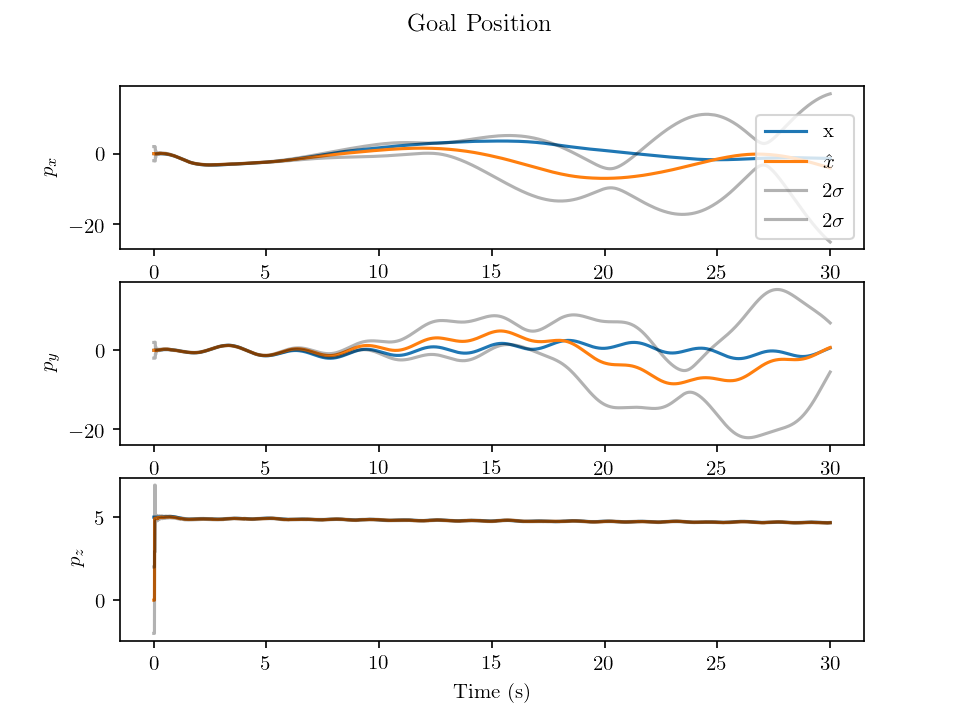
\includegraphics[scale=0.5]{plots/no_lms_gp.png}
  \caption{Simulation results with the estimator using no visual
  features. The blue line represents the true state while the orange line
  represents the estimated state. The two grey lines show a 2 $\sigma$ bound for
  the estimate based on the estimated covariance. Measurements from the fiducial
  marker are not used after $t$~=~5
$s$ to demonstrate the performance of the estimator.}
  \label{fig:no_lms_gp}
\end{figure}

\begin{figure}
  \centering
  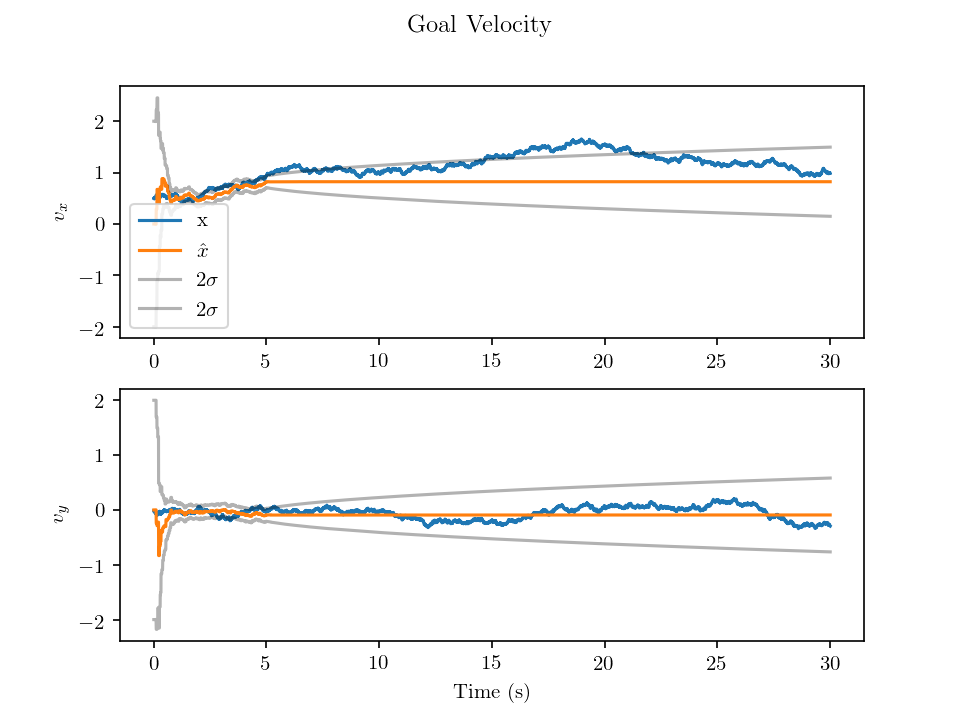
\includegraphics[scale=0.5]{plots/no_lms_gv.png}
  \caption{Simulation results with the estimator using no visual
  features. The blue line represents the true state while the orange line
  represents the estimated state. The two grey lines show a 2 $\sigma$ bound for
  the estimate based on the estimated covariance. Measurements from the fiducial
  marker are not used after $t$~=~5
$s$ to demonstrate the performance of the estimator.}
  \label{fig:no_lms_gv}
\end{figure}

\begin{figure}
  \centering
  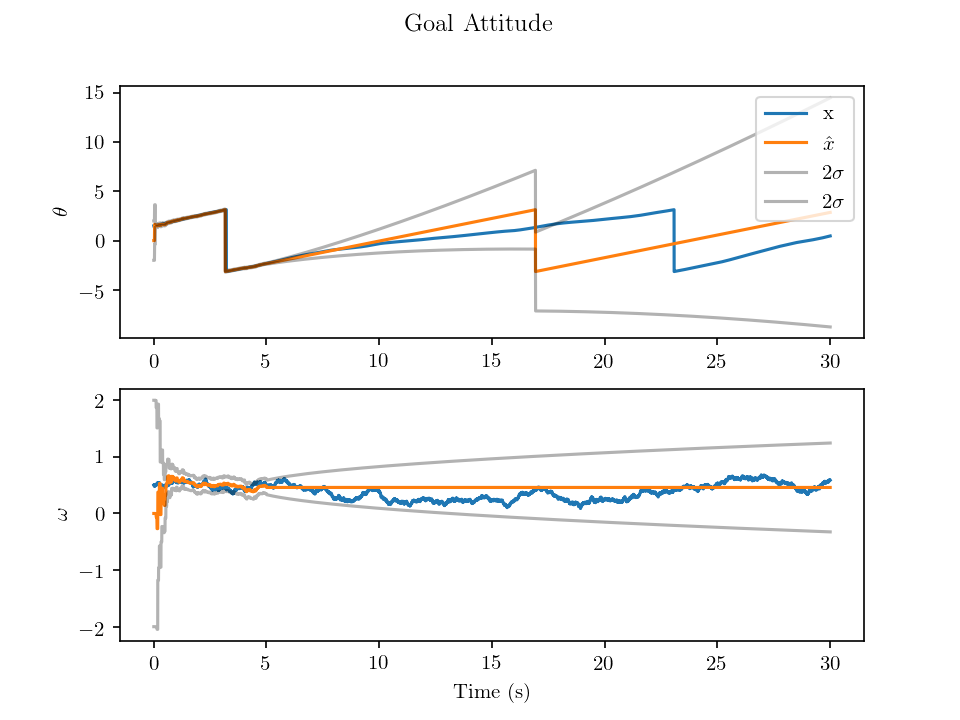
\includegraphics[scale=0.5]{plots/no_lms_gatt.png}
  \caption{Simulation results with the estimator using no visual
  features. The blue line represents the true state while the orange line
  represents the estimated state. The two grey lines show a 2 $\sigma$ bound for
  the estimate based on the estimated covariance. Measurements from the fiducial
  marker are not used after $t$~=~5
$s$ to demonstrate the performance of the estimator.}
  \label{fig:no_lms_gatt}
\end{figure}

\begin{figure}
  \centering
  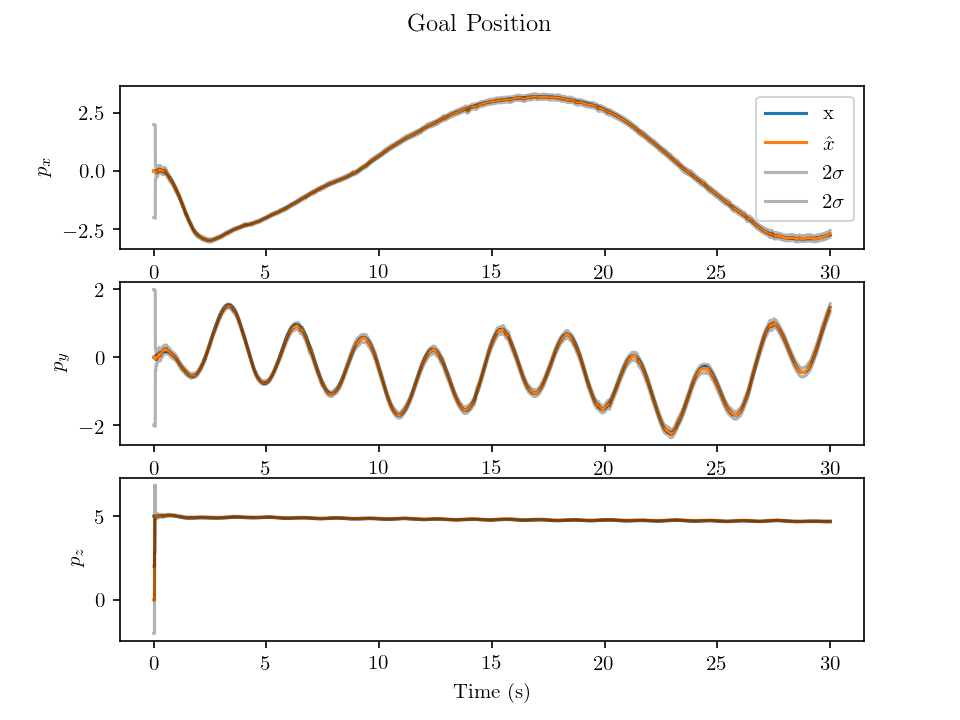
\includegraphics[scale=0.5]{plots/with_lms_gp.png}
  \caption{Simulation results with estimator using a maximum of ten visual
  features. Measurements from the fiducial marker are not used after $t$ = 5
$s$ to demonstrate the performance of the estimator.}
  \label{fig:with_lms_gp}
\end{figure}

\begin{figure}
  \centering
  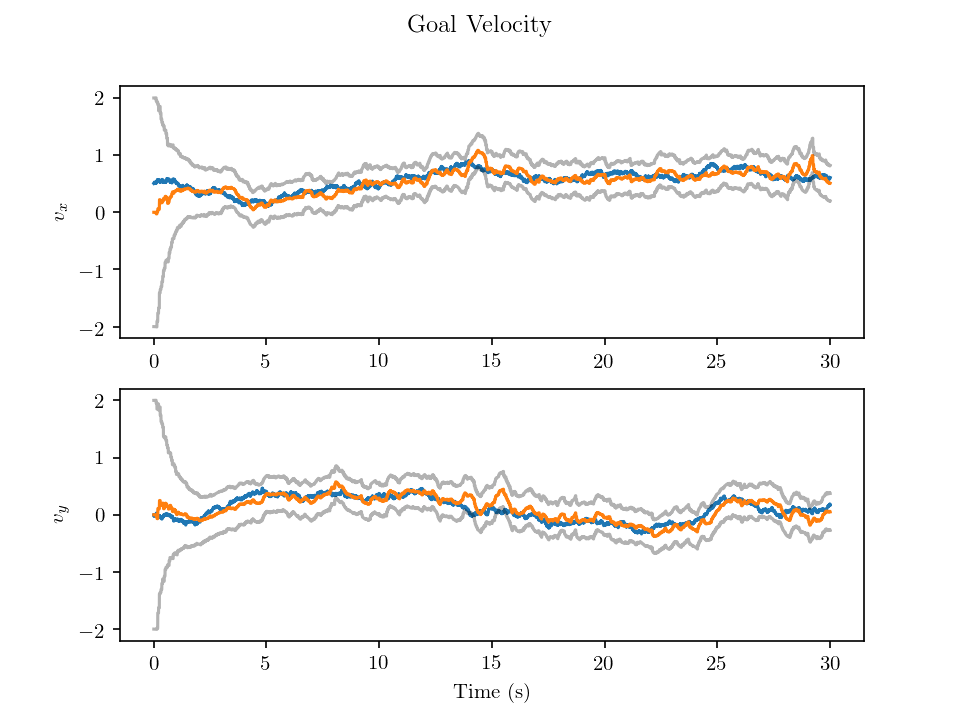
\includegraphics[scale=0.5]{plots/with_lms_gv.png}
  \caption{Simulation results with estimator using a maximum of ten visual
  features. Measurements from the fiducial marker are not used after $t$ = 5
$s$ to demonstrate the performance of the estimator.}
  \label{fig:with_lms_gv}
\end{figure}

\begin{figure}
  \centering
  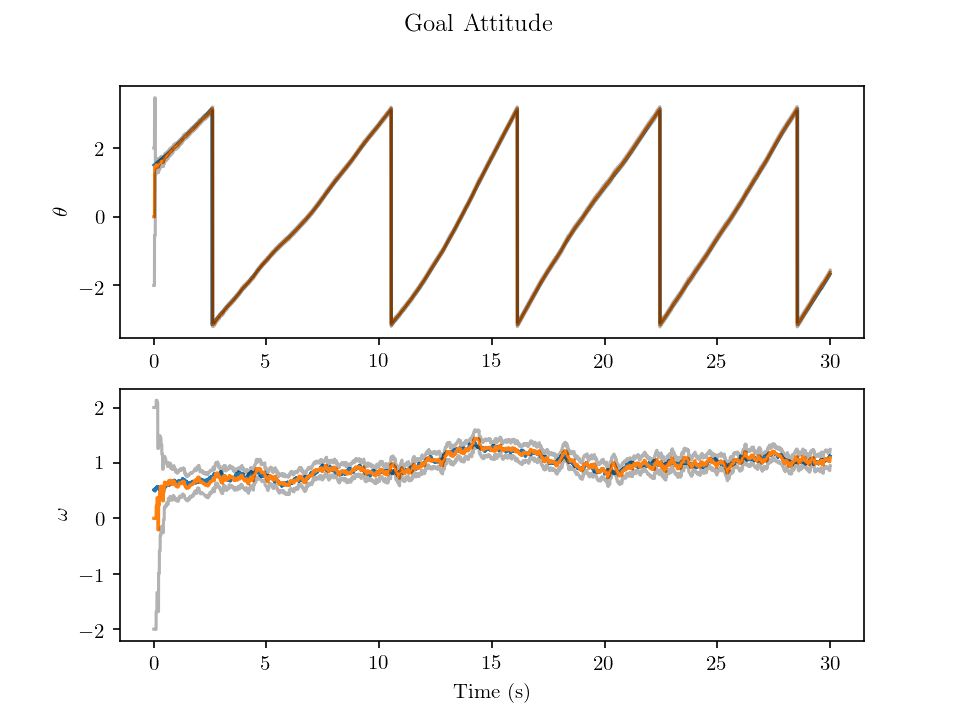
\includegraphics[scale=0.5]{plots/with_lms_gatt.png}
  \caption{Simulation results with estimator using a maximum of ten visual
  features. Measurements from the fiducial marker are not used after $t$ = 5
$s$ to demonstrate the performance of the estimator.}
  \label{fig:with_lms_gatt}
\end{figure}


\begin{figure}
  \centering
  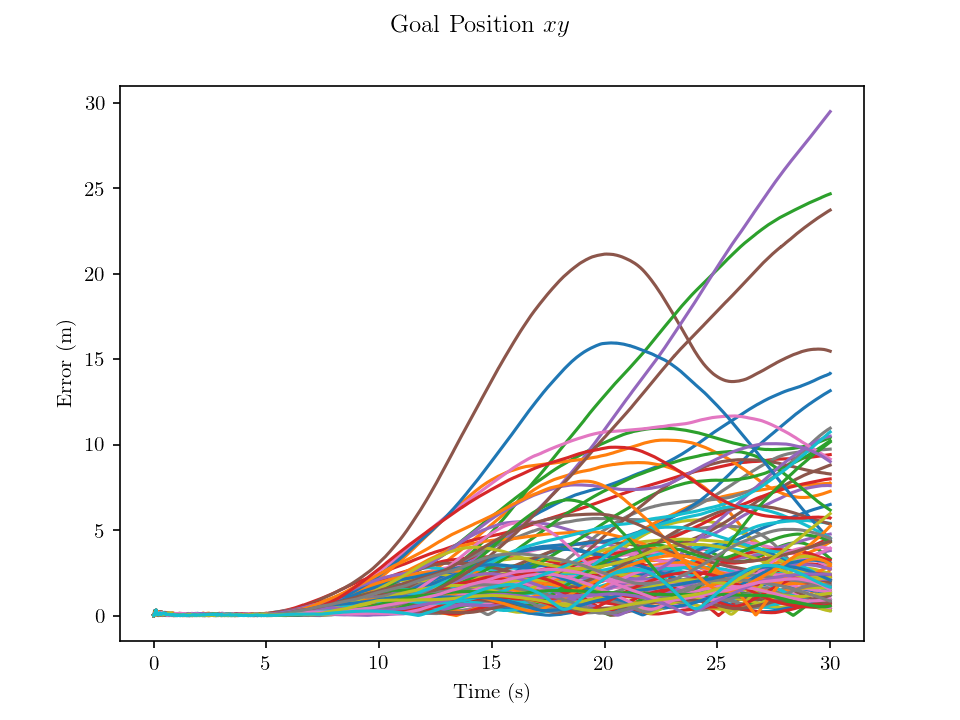
\includegraphics[scale=0.5]{plots/mc_no_lms_xy_err.png}
  \caption{Simulation results with estimator using no visual
  features. Measurements from the fiducial marker are not used after $t$ = 5
$s$ to demonstrate the performance of the estimator. The L2 norm of the error in
the x and y directions of the goal position is seen for 100 different simulation
runs.}
  \label{fig:mc_no_lms_xy_err}
\end{figure}

\begin{figure}
  \centering
  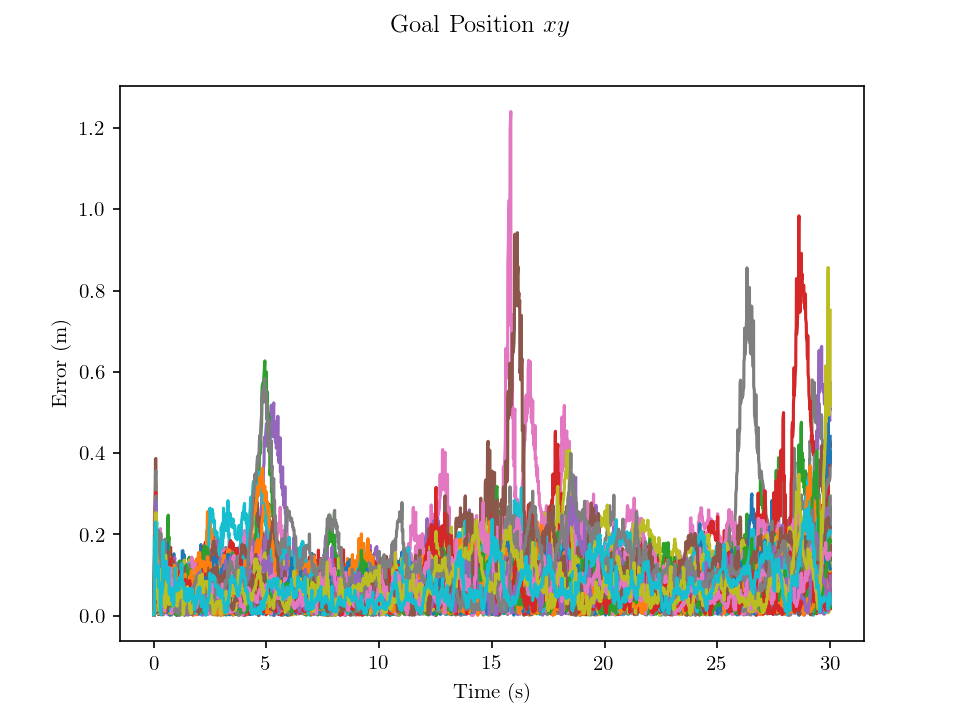
\includegraphics[scale=0.5]{plots/mc_with_lms_xy_err.png}
  \caption{Simulation results with estimator using a maximum of ten visual
  features. Measurements from the fiducial marker are not used after $t$ = 5
$s$ to demonstrate the performance of the estimator. The L2 norm of the error in
the x and y directions of the goal position is seen for 100 different simulation
runs.}
  \label{fig:mc_with_lms_xy_err}
\end{figure}



\section{Hardware} \label{sec:hardware}
% !TEX root=../root.tex

\subsection{Platform}
The proposed estimation algorithm was implemented and flown in
hardware to further demonstrate the performance observed in the simulation
results. The multirotor used for experiments was built on a DJI 450 Flamewheel
frame. All computation was done onboard the UAV on an NVIDIA Jetson TX2 using
ROS. An ELP
USB Camera with a 2.1mm Lens was mounted to the bottom of the UAV such that the
camera faced downward in the UAV's bodyframe.

A successive loop PID control scheme was used to close the loop around the
estimated states. Throughout the flight, the UAV was commanded to maintain a
constant altitude relative to the goal frame of 0.5 $m$ while attempting to
drive the $x$ and $y$ components of $\vect{p}_{g/b}^v$ to zero. The relative yaw
angle between the UAV and the goal frame was also controlled to zero.
Controller commands were sent from
the onboard computer to the CC3D Revolution 32bit F4 flight controller running
the ROSflight firmware~\cite{jackson2016rosflight}.


% % !TEX root=../root.tex

\subsection{Control}
Simple nested PID control. Maintain constant relative altitude. Control
$\vect{p}_{g/b}^v$ to zero

% !TEX root=../root.tex

% \subsection{Fiducial Landing Marker}
The fiducial landing marker used in our flight experiments was a 6.1 cm $\times$ 6.1 cm ArUco
marker~\cite{romero2018speeded}, as pictured in the top, right corner
of~\figref{fig:features_with_aruco}.
% We use an ArUco marker~\cite{romero2018speeded}, as pictured in the upper, right
% of~\figref{fig:features_with_aruco}, for the fiducial landing marker
When detected in a camera image, a relative translation and
rotation from the camera frame to the marker was estimated using the detected positions of
the corners of the marker in the camera image and the known size of the marker. 
% The ArUco library used only detects the marker when it is entirely visible, and
% unobstructed in the camera image.
% Due to these
% conditions, it is not uncommon that the marker may be undetected for significant
% periods of time during a landing maneuver.


% !TEX root=../root.tex

\subsection{Feature Tracking}
As mentioned in~\secref{sec:estimation},
the estimation algorithm uses measurements of visual features that are
rigidly attached to the landing target vehicle. It is important to note that
determining which visual features in a camera image are attached to
the target vehicle is not a trivial problem. We leave this problem as future work and
circumvent this problem by flying low enough to the target vehicle such that it
occupies the entire field of view of the camera.

Visual features were first detected using a FAST feature
detector~\cite{rosten2006machine}. The detected features were then tracked from one frame to
the next using optical flow~\cite{bouguet2001pyramidal}.
To remove features that had been poorly tracked, we periodically
estimated the essential matrix between the current camera image
and a stored keyframe.
Outliers to this estimated essential matrix were discarded, and new FAST
features were detected to replace them.
% to have been poorly tracked
% Periodically, we
% removed
% features that had been poorly tracked by estimating the essential matrix between
% the current camera image and a stored keyframe image. Outliers to the found
% essential matrix were thrown out, and new FAST features were detected to replace
% them. 
For our experiments, the feature tracker attempted to maintain 250
tracked features at all times. As the proposed estimator only used ten visual
features at a time,
% measurements from a few
% tracked features,
a subset of the tracked features which had persisted the longest
were provided to the estimator for each camera image.

Each visual feature that was acquired and tracked was assigned a unique integer
identitication number. The estimator used these identification numbers to
determine when visual features were no longer tracked and when new visual
features were acquired.
% a visual feature was no longer tracked and, therefore, should
% have been removed from
% the estimated state.
An example camera image from the UAV showing the
subset of tracked features provided to the estimator with the corresponding
identification
numbers is seen in~\figref{fig:features_with_aruco}.


\begin{figure}
  \centering
  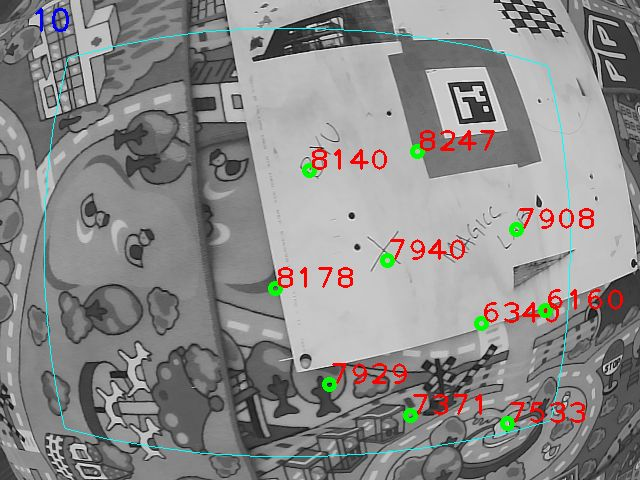
\includegraphics[scale=0.5]{imgs/features_with_aruco.png}
  \caption[Visual Feature Tracking During Flight Experiment]{A processed camera
    image from the multirotor UAV's camera where the landing target vehicle
    occupies the entire image. The ArUco
  marker is pictured in the top, right corner of the image. Each green
circle shows the tracked location of a visual feature used by the
estimator. The red number associated with each visual feature is the unique
integer ID assigned by the feature tracker.}
  \label{fig:features_with_aruco}
\end{figure}

% !TEX root=../root.tex

\subsection{Indoor Motion Capture}
The hardware flight experiments were conducted in the indoor motion capture room
in the MAGICC Lab at Brigham Young University. An Optitrack motion capture
system provides meaurements of the global position and attitude of the UAV
throughout the flights.


% !TEX root=../root.tex

\subsection{Landing Target Vehicle}
As flight tests were conducted in a small indoor environment,
the landing target
vehicle was designed to be small in an attempt to better extend to outdoor
scenarios in which the UAV is to land on larger vehicles such as trucks or boats.
The target vehicle, pictured in~\figref{fig:landing_vehicle}, was manually
driven during the experiments,
rougly following an oval.
% following a rough oval.
% A ground vehicle was assembled as pictured in~\figref{fig:landing_vehicle}
% % with a
% % 6.1 $cm$ ArUco tag serving as the fiducial landing marker.
% % During the experiments, the landing vehicle was
% and manually driven around the
% perimeter of the room during the experiments.

\begin{figure}
  \centering
  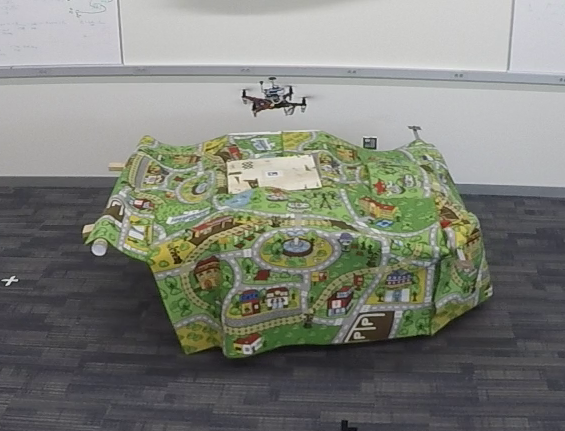
\includegraphics[scale=0.5]{imgs/landing_vehicle.png}
  \caption[UAV Tracking the Target Vehicle During Flight Experiment]{Multirotor
    UAV shown in autonomous flight, tracking the landing target
  vehicle.}
  \label{fig:landing_vehicle}
\end{figure}

% !TEX root=../root.tex

\subsection{Experiment Results}
% The multirotor UAV was manually flown until the
% fiducial landing marker was detected. Upon detection, the closed-loop estimation
% and control system took full control of the UAV.

The results of the flight experiment are shown in~\figref{fig:est_hardware}.
The fiducial landing marker was first detected at $t = 20$ s, where the plots
begin.
To demonstrate the ability of the
system to maintain good tracking of a target vehicle when a fiducial
marker is not detected for long periods of time, the fiducial marker detection
was turned off ten seconds after initial detection, at $t = 30$ s.
% The fiducial landing marker was first detected at
% $t = 20$ s and last detected at $t = 30$ s.
It is clear that the estimates of the position, velocity, attitude, and angular
velocity of the target vehicle remained accurate and consistent for the duration
of the experiment.
% despite no measurements from the fiducial marker being used
% after $t = 30$ s.
% Even though no measurements from the fiducial marker are used, it is clear that
% the estimates of the position, velocitity, attitude and angular velocity of the
% target vehicle remain accurate and consistent for the duration of the
% experiment.
These accurate estimates allowed
the UAV to continue to control relative to the target vehicle, tracking closely
above the landing target as the target vehicle moved around the room. After the
target vehicle completed two full laps around the room,
at approximately $t=102$ s, manual control of the UAV was resumed, ending the experiment.
A video of the flight experiment can be found at
\url{https://youtu.be/3AyjCI0c1Nc}.
% \url{https://youtu.be/VU5sq6FuSL0}.

\begin{figure}
  \centering
  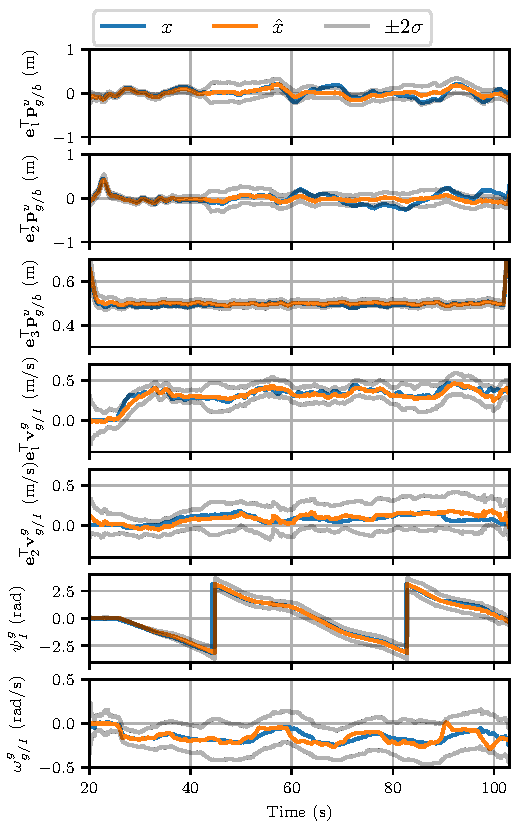
\includegraphics[width=6.5in]{plots/hardware_results}
  \caption[ESKF Hardware Results Using Ten Visual Features]{Hardware results when
    the ESKF estimated the positions of \emph{ten} visual
  features. The blue line represents the true state while the orange line
  represents the estimated state. The two grey lines show $\pm 2 \sigma$ bounds for
  the estimate based on the estimated covariance. Measurements from the fiducial
  marker were not used after $t = 30$ s to demonstrate the performance of the estimator.}
  \label{fig:est_hardware}
\end{figure}


\section{Conclusion} \label{sec:conclusion}
The proposed estimator provides a method for maintaining accurate and consistent
estimates of the state of a landing vehicle when a fiducial landing marker is
not detected for significant periods of time. This improvement is achieved by
tracking and estimating the locations of unknown visual landmarks on the landing
vehicle. The simulation and hardware experiments show that by tracking and
estimating the locations of just 10 visual landmarks, the multirotor UAV can
continue to reliably operate with respect to the landing vehicle for long
periods of time without detecting the fiducial landing marker.

% \appendices
% \section{Proof of the First Zonklar Equation}
% Appendix one text goes here.

% \section{}
% Appendix two text goes here.

% \section*{Acknowledgment}
% The authors would like to thank...

\bibliographystyle{IEEEtran}
\bibliography{abbrev,library}

\end{document}


